% Options for packages loaded elsewhere
\PassOptionsToPackage{unicode}{hyperref}
\PassOptionsToPackage{hyphens}{url}
%
\documentclass[
]{book}
\usepackage{lmodern}
\usepackage{amssymb,amsmath}
\usepackage{ifxetex,ifluatex}
\ifnum 0\ifxetex 1\fi\ifluatex 1\fi=0 % if pdftex
  \usepackage[T1]{fontenc}
  \usepackage[utf8]{inputenc}
  \usepackage{textcomp} % provide euro and other symbols
\else % if luatex or xetex
  \usepackage{unicode-math}
  \defaultfontfeatures{Scale=MatchLowercase}
  \defaultfontfeatures[\rmfamily]{Ligatures=TeX,Scale=1}
\fi
% Use upquote if available, for straight quotes in verbatim environments
\IfFileExists{upquote.sty}{\usepackage{upquote}}{}
\IfFileExists{microtype.sty}{% use microtype if available
  \usepackage[]{microtype}
  \UseMicrotypeSet[protrusion]{basicmath} % disable protrusion for tt fonts
}{}
\makeatletter
\@ifundefined{KOMAClassName}{% if non-KOMA class
  \IfFileExists{parskip.sty}{%
    \usepackage{parskip}
  }{% else
    \setlength{\parindent}{0pt}
    \setlength{\parskip}{6pt plus 2pt minus 1pt}}
}{% if KOMA class
  \KOMAoptions{parskip=half}}
\makeatother
\usepackage{xcolor}
\IfFileExists{xurl.sty}{\usepackage{xurl}}{} % add URL line breaks if available
\IfFileExists{bookmark.sty}{\usepackage{bookmark}}{\usepackage{hyperref}}
\hypersetup{
  pdftitle={Applied Spatial Data Analysis - Spatial Point and Lattice Data},
  pdfauthor={Dr Sebnem Er},
  hidelinks,
  pdfcreator={LaTeX via pandoc}}
\urlstyle{same} % disable monospaced font for URLs
\usepackage{color}
\usepackage{fancyvrb}
\newcommand{\VerbBar}{|}
\newcommand{\VERB}{\Verb[commandchars=\\\{\}]}
\DefineVerbatimEnvironment{Highlighting}{Verbatim}{commandchars=\\\{\}}
% Add ',fontsize=\small' for more characters per line
\usepackage{framed}
\definecolor{shadecolor}{RGB}{248,248,248}
\newenvironment{Shaded}{\begin{snugshade}}{\end{snugshade}}
\newcommand{\AlertTok}[1]{\textcolor[rgb]{0.94,0.16,0.16}{#1}}
\newcommand{\AnnotationTok}[1]{\textcolor[rgb]{0.56,0.35,0.01}{\textbf{\textit{#1}}}}
\newcommand{\AttributeTok}[1]{\textcolor[rgb]{0.77,0.63,0.00}{#1}}
\newcommand{\BaseNTok}[1]{\textcolor[rgb]{0.00,0.00,0.81}{#1}}
\newcommand{\BuiltInTok}[1]{#1}
\newcommand{\CharTok}[1]{\textcolor[rgb]{0.31,0.60,0.02}{#1}}
\newcommand{\CommentTok}[1]{\textcolor[rgb]{0.56,0.35,0.01}{\textit{#1}}}
\newcommand{\CommentVarTok}[1]{\textcolor[rgb]{0.56,0.35,0.01}{\textbf{\textit{#1}}}}
\newcommand{\ConstantTok}[1]{\textcolor[rgb]{0.00,0.00,0.00}{#1}}
\newcommand{\ControlFlowTok}[1]{\textcolor[rgb]{0.13,0.29,0.53}{\textbf{#1}}}
\newcommand{\DataTypeTok}[1]{\textcolor[rgb]{0.13,0.29,0.53}{#1}}
\newcommand{\DecValTok}[1]{\textcolor[rgb]{0.00,0.00,0.81}{#1}}
\newcommand{\DocumentationTok}[1]{\textcolor[rgb]{0.56,0.35,0.01}{\textbf{\textit{#1}}}}
\newcommand{\ErrorTok}[1]{\textcolor[rgb]{0.64,0.00,0.00}{\textbf{#1}}}
\newcommand{\ExtensionTok}[1]{#1}
\newcommand{\FloatTok}[1]{\textcolor[rgb]{0.00,0.00,0.81}{#1}}
\newcommand{\FunctionTok}[1]{\textcolor[rgb]{0.00,0.00,0.00}{#1}}
\newcommand{\ImportTok}[1]{#1}
\newcommand{\InformationTok}[1]{\textcolor[rgb]{0.56,0.35,0.01}{\textbf{\textit{#1}}}}
\newcommand{\KeywordTok}[1]{\textcolor[rgb]{0.13,0.29,0.53}{\textbf{#1}}}
\newcommand{\NormalTok}[1]{#1}
\newcommand{\OperatorTok}[1]{\textcolor[rgb]{0.81,0.36,0.00}{\textbf{#1}}}
\newcommand{\OtherTok}[1]{\textcolor[rgb]{0.56,0.35,0.01}{#1}}
\newcommand{\PreprocessorTok}[1]{\textcolor[rgb]{0.56,0.35,0.01}{\textit{#1}}}
\newcommand{\RegionMarkerTok}[1]{#1}
\newcommand{\SpecialCharTok}[1]{\textcolor[rgb]{0.00,0.00,0.00}{#1}}
\newcommand{\SpecialStringTok}[1]{\textcolor[rgb]{0.31,0.60,0.02}{#1}}
\newcommand{\StringTok}[1]{\textcolor[rgb]{0.31,0.60,0.02}{#1}}
\newcommand{\VariableTok}[1]{\textcolor[rgb]{0.00,0.00,0.00}{#1}}
\newcommand{\VerbatimStringTok}[1]{\textcolor[rgb]{0.31,0.60,0.02}{#1}}
\newcommand{\WarningTok}[1]{\textcolor[rgb]{0.56,0.35,0.01}{\textbf{\textit{#1}}}}
\usepackage{longtable,booktabs}
% Correct order of tables after \paragraph or \subparagraph
\usepackage{etoolbox}
\makeatletter
\patchcmd\longtable{\par}{\if@noskipsec\mbox{}\fi\par}{}{}
\makeatother
% Allow footnotes in longtable head/foot
\IfFileExists{footnotehyper.sty}{\usepackage{footnotehyper}}{\usepackage{footnote}}
\makesavenoteenv{longtable}
\usepackage{graphicx,grffile}
\makeatletter
\def\maxwidth{\ifdim\Gin@nat@width>\linewidth\linewidth\else\Gin@nat@width\fi}
\def\maxheight{\ifdim\Gin@nat@height>\textheight\textheight\else\Gin@nat@height\fi}
\makeatother
% Scale images if necessary, so that they will not overflow the page
% margins by default, and it is still possible to overwrite the defaults
% using explicit options in \includegraphics[width, height, ...]{}
\setkeys{Gin}{width=\maxwidth,height=\maxheight,keepaspectratio}
% Set default figure placement to htbp
\makeatletter
\def\fps@figure{htbp}
\makeatother
\setlength{\emergencystretch}{3em} % prevent overfull lines
\providecommand{\tightlist}{%
  \setlength{\itemsep}{0pt}\setlength{\parskip}{0pt}}
\setcounter{secnumdepth}{5}
\usepackage{booktabs}
\usepackage{amsthm}
\makeatletter
\def\thm@space@setup{%
  \thm@preskip=8pt plus 2pt minus 4pt
  \thm@postskip=\thm@preskip
}
\makeatother
\usepackage[]{natbib}
\bibliographystyle{apalike}

\title{Applied Spatial Data Analysis - Spatial Point and Lattice Data}
\author{Dr Sebnem Er}
\date{2020-10-04}

\begin{document}
\maketitle

{
\setcounter{tocdepth}{1}
\tableofcontents
}
\hypertarget{introduction}{%
\chapter{Introduction}\label{introduction}}

This book will guide you through the R codes for Spatial Point and Lattice Data Analysis.

The chapters will be made available on Tuesdays when we start a new week So please update your browser to access the codes for the relevant chapter.

\hypertarget{spatial-point-pattern-analysis}{%
\chapter{Spatial Point Pattern Analysis}\label{spatial-point-pattern-analysis}}

\hypertarget{prerequisites}{%
\section{Prerequisites}\label{prerequisites}}

You need to have the following R packages installed and recalled into your library:

\begin{Shaded}
\begin{Highlighting}[]
\KeywordTok{library}\NormalTok{(sf)}
\KeywordTok{library}\NormalTok{(spatstat)}
\KeywordTok{library}\NormalTok{(spatstat.data)}
\KeywordTok{library}\NormalTok{(ggplot2)}
\KeywordTok{library}\NormalTok{(sp)}
\KeywordTok{library}\NormalTok{(animation)}
\KeywordTok{library}\NormalTok{(plotrix)}
\end{Highlighting}
\end{Shaded}

\hypertarget{datasets---readily-available-imported-simulated-datasets}{%
\section{Datasets - Readily Available, Imported, Simulated Datasets}\label{datasets---readily-available-imported-simulated-datasets}}

\hypertarget{swedishpines-dataset-from-spatstat.data-library}{%
\subsection{Swedishpines Dataset from spatstat.data library}\label{swedishpines-dataset-from-spatstat.data-library}}

\begin{Shaded}
\begin{Highlighting}[]
\KeywordTok{data}\NormalTok{(swedishpines)}
\NormalTok{swp =}\StringTok{ }\NormalTok{spatstat}\OperatorTok{::}\KeywordTok{rescale}\NormalTok{(swedishpines)}
\KeywordTok{class}\NormalTok{(swp)}
\end{Highlighting}
\end{Shaded}

\begin{verbatim}
## [1] "ppp"
\end{verbatim}

\begin{Shaded}
\begin{Highlighting}[]
\KeywordTok{summary}\NormalTok{(swp)}
\end{Highlighting}
\end{Shaded}

\begin{verbatim}
## Planar point pattern:  71 points
## Average intensity 0.7395833 points per square metre
## 
## Coordinates are given to 1 decimal place
## i.e. rounded to the nearest multiple of 0.1 metres
## 
## Window: rectangle = [0, 9.6] x [0, 10] metres
## Window area = 96 square metres
## Unit of length: 1 metre
\end{verbatim}

\begin{Shaded}
\begin{Highlighting}[]
\KeywordTok{plot}\NormalTok{(swp)}
\end{Highlighting}
\end{Shaded}

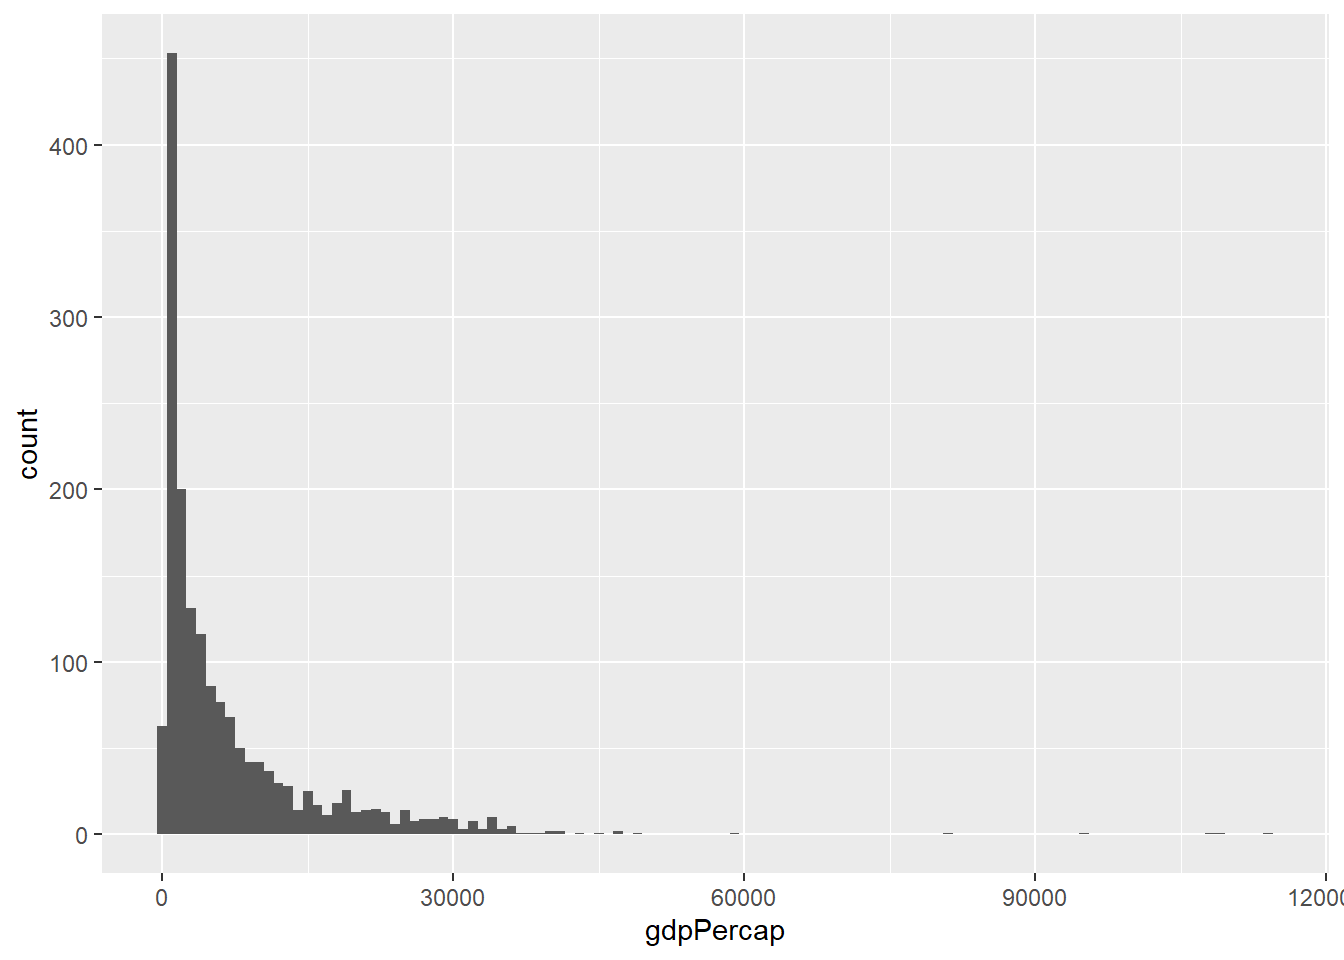
\includegraphics{Applied-Spatial-Data-Analysis_files/figure-latex/unnamed-chunk-2-1.pdf}

\hypertarget{clinics-dataset-using-simple-features-sf}{%
\subsection{Clinics Dataset Using Simple Features (SF)}\label{clinics-dataset-using-simple-features-sf}}

Download the data from the following:

\url{https://web1.capetown.gov.za/web1/OpenDataPortal/DatasetDetail?DatasetName=Clinics}

Extract the data frame into R:

\begin{Shaded}
\begin{Highlighting}[]
\KeywordTok{library}\NormalTok{(sf)}
\NormalTok{clinics_sf =}\StringTok{ }\KeywordTok{st_read}\NormalTok{(}\StringTok{"C:/Users/01438475/Google Drive/UCTcourses/ASDA/DataSets/Clinics/SL_CLNC.shp"}\NormalTok{)}
\end{Highlighting}
\end{Shaded}

\begin{verbatim}
## Reading layer `SL_CLNC' from data source `C:\Users\01438475\Google Drive\UCTcourses\ASDA\DataSets\Clinics\SL_CLNC.shp' using driver `ESRI Shapefile'
## Simple feature collection with 149 features and 5 fields
## geometry type:  POINT
## dimension:      XY
## bbox:           xmin: 18.34268 ymin: -34.19491 xmax: 18.90847 ymax: -33.51262
## geographic CRS: WGS 84
\end{verbatim}

\begin{Shaded}
\begin{Highlighting}[]
\NormalTok{clinics_sf}
\end{Highlighting}
\end{Shaded}

\begin{verbatim}
## Simple feature collection with 149 features and 5 fields
## geometry type:  POINT
## dimension:      XY
## bbox:           xmin: 18.34268 ymin: -34.19491 xmax: 18.90847 ymax: -33.51262
## geographic CRS: WGS 84
## First 10 features:
##                                        LCTN              ATHY
## 1           C/O Adam/ Liedeman Street Mamre              PAWC
## 2                 Cnr Hermes & GrosvenorAve CITY OF CAPE TOWN
## 3            Hassen Kahn Ave Rusthof Strand              PAWC
## 4              61 Central Circle, Fish Hoek CITY OF CAPE TOWN
## 5                     Simon Street, Nomzamo CITY OF CAPE TOWN
## 6  C/O Musical and Hospital Street Macassar              PAWC
## 7            28 Church Street Somerset West CITY OF CAPE TOWN
## 8                       Fagan Street Strand CITY OF CAPE TOWN
## 9    Karbonkel Road, CMC Building, Hout Bay              PAWC
## 10                Midmar Street Groenvallei CITY OF CAPE TOWN
##                      NAME                CLASS       RGN
## 1               MAMRE CDC Community Day Centre   Western
## 2        SAXON SEA CLINIC               Clinic   Western
## 3            GUSTROUW CDC Community Day Centre   Eastern
## 4        FISH HOEK CLINIC               Clinic  Southern
## 5              IKWEZI CDC Community Day Centre   Eastern
## 6            MACASSAR CDC Community Day Centre   Eastern
## 7    SOMERSET WEST CLINIC               Clinic   Eastern
## 8  FAGAN STREET SATELLITE            Satellite   Eastern
## 9    HOUT BAY HARBOUR CDC Community Day Centre  Southern
## 10  GROENVALLEI SATELLITE            Satellite Tygerberg
##                      geometry
## 1  POINT (18.47692 -33.51262)
## 2  POINT (18.48881 -33.55012)
## 3  POINT (18.85211 -34.13472)
## 4  POINT (18.42632 -34.13669)
## 5  POINT (18.86622 -34.11375)
## 6  POINT (18.76369 -34.06105)
## 7  POINT (18.84814 -34.08579)
## 8   POINT (18.82979 -34.1162)
## 9   POINT (18.34268 -34.0549)
## 10 POINT (18.66701 -33.89165)
\end{verbatim}

\begin{Shaded}
\begin{Highlighting}[]
\KeywordTok{class}\NormalTok{(clinics_sf)}
\end{Highlighting}
\end{Shaded}

\begin{verbatim}
## [1] "sf"         "data.frame"
\end{verbatim}

\begin{Shaded}
\begin{Highlighting}[]
\KeywordTok{summary}\NormalTok{(clinics_sf)}
\end{Highlighting}
\end{Shaded}

\begin{verbatim}
##      LCTN               ATHY               NAME              CLASS          
##  Length:149         Length:149         Length:149         Length:149        
##  Class :character   Class :character   Class :character   Class :character  
##  Mode  :character   Mode  :character   Mode  :character   Mode  :character  
##      RGN                     geometry  
##  Length:149         POINT        :149  
##  Class :character   epsg:4326    :  0  
##  Mode  :character   +proj=long...:  0
\end{verbatim}

\hypertarget{simulated-datasets}{%
\subsection{Simulated Datasets}\label{simulated-datasets}}

\hypertarget{csr-data-points}{%
\subsubsection{CSR Data Points}\label{csr-data-points}}

\begin{Shaded}
\begin{Highlighting}[]
\KeywordTok{set.seed}\NormalTok{(}\DecValTok{135}\NormalTok{)}
\NormalTok{xy_csr <-}\StringTok{ }\KeywordTok{matrix}\NormalTok{(}\KeywordTok{runif}\NormalTok{(}\DecValTok{80}\NormalTok{), }\DataTypeTok{ncol=}\DecValTok{2}\NormalTok{)}
\NormalTok{pp_csr <-}\StringTok{ }\KeywordTok{as.ppp}\NormalTok{(xy_csr, }\KeywordTok{c}\NormalTok{(}\DecValTok{0}\NormalTok{,}\DecValTok{1}\NormalTok{,}\DecValTok{0}\NormalTok{,}\DecValTok{1}\NormalTok{))}
\KeywordTok{plot}\NormalTok{(pp_csr)}
\end{Highlighting}
\end{Shaded}

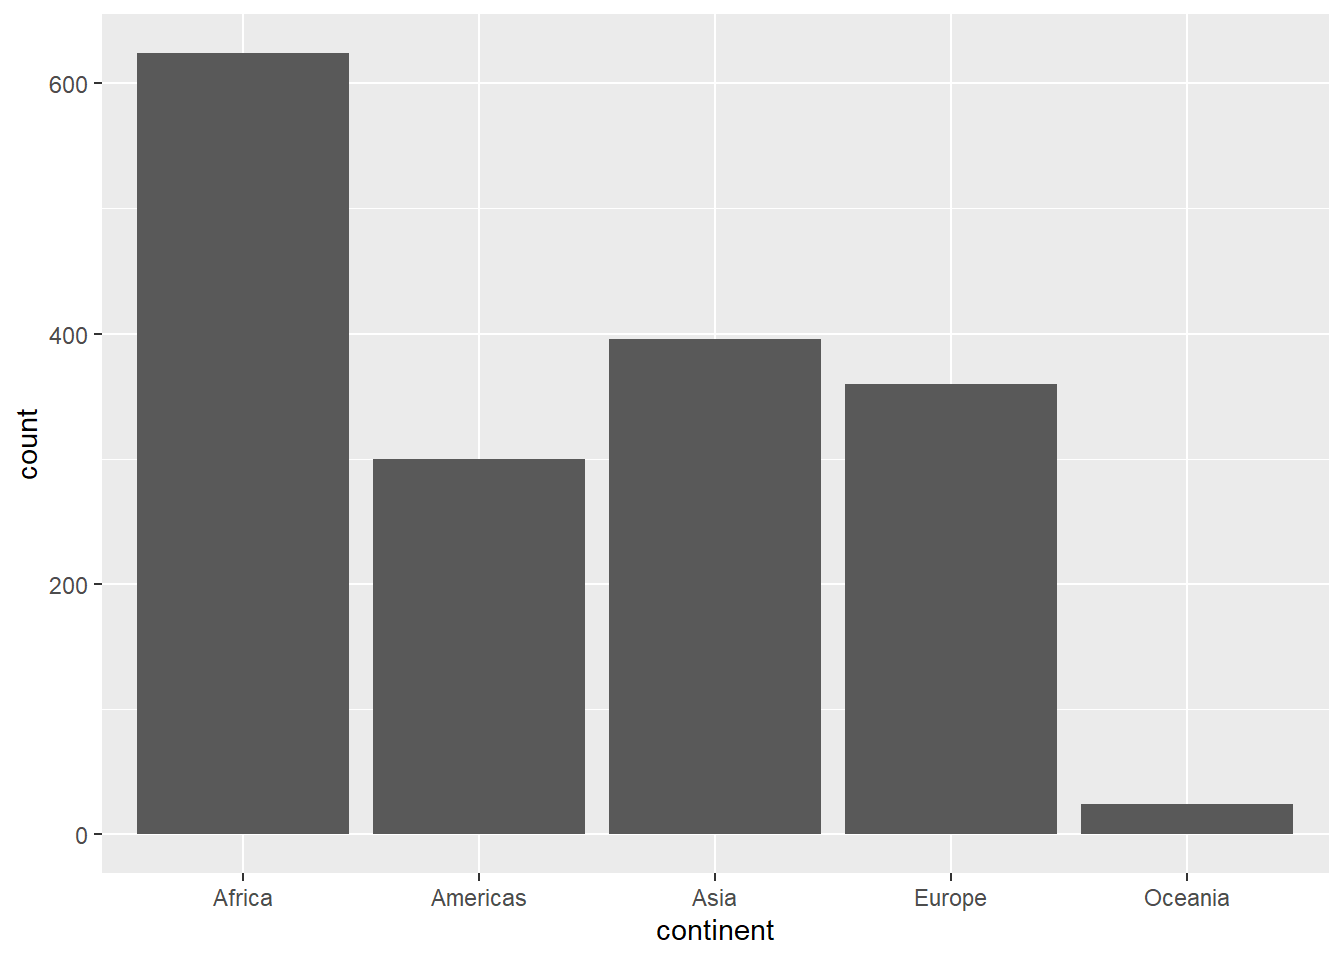
\includegraphics{Applied-Spatial-Data-Analysis_files/figure-latex/unnamed-chunk-4-1.pdf}

\hypertarget{regular-data-points}{%
\subsubsection{Regular Data Points}\label{regular-data-points}}

\begin{Shaded}
\begin{Highlighting}[]
\NormalTok{regular <-}\StringTok{ }\KeywordTok{read.csv}\NormalTok{(}\StringTok{"C:/Users/01438475/Google Drive/UCTcourses/ASDA/regular.csv"}\NormalTok{)}
\NormalTok{xy_regular <-}\StringTok{ }\KeywordTok{matrix}\NormalTok{(}\KeywordTok{cbind}\NormalTok{(regular}\OperatorTok{$}\NormalTok{X,regular}\OperatorTok{$}\NormalTok{Y), }\DataTypeTok{ncol=}\DecValTok{2}\NormalTok{)}
\NormalTok{pp_regular <-}\StringTok{ }\KeywordTok{as.ppp}\NormalTok{(xy_regular, }\KeywordTok{c}\NormalTok{(}\DecValTok{0}\NormalTok{,}\DecValTok{1}\NormalTok{,}\DecValTok{0}\NormalTok{,}\DecValTok{1}\NormalTok{))}
\KeywordTok{plot}\NormalTok{(pp_regular)}
\end{Highlighting}
\end{Shaded}

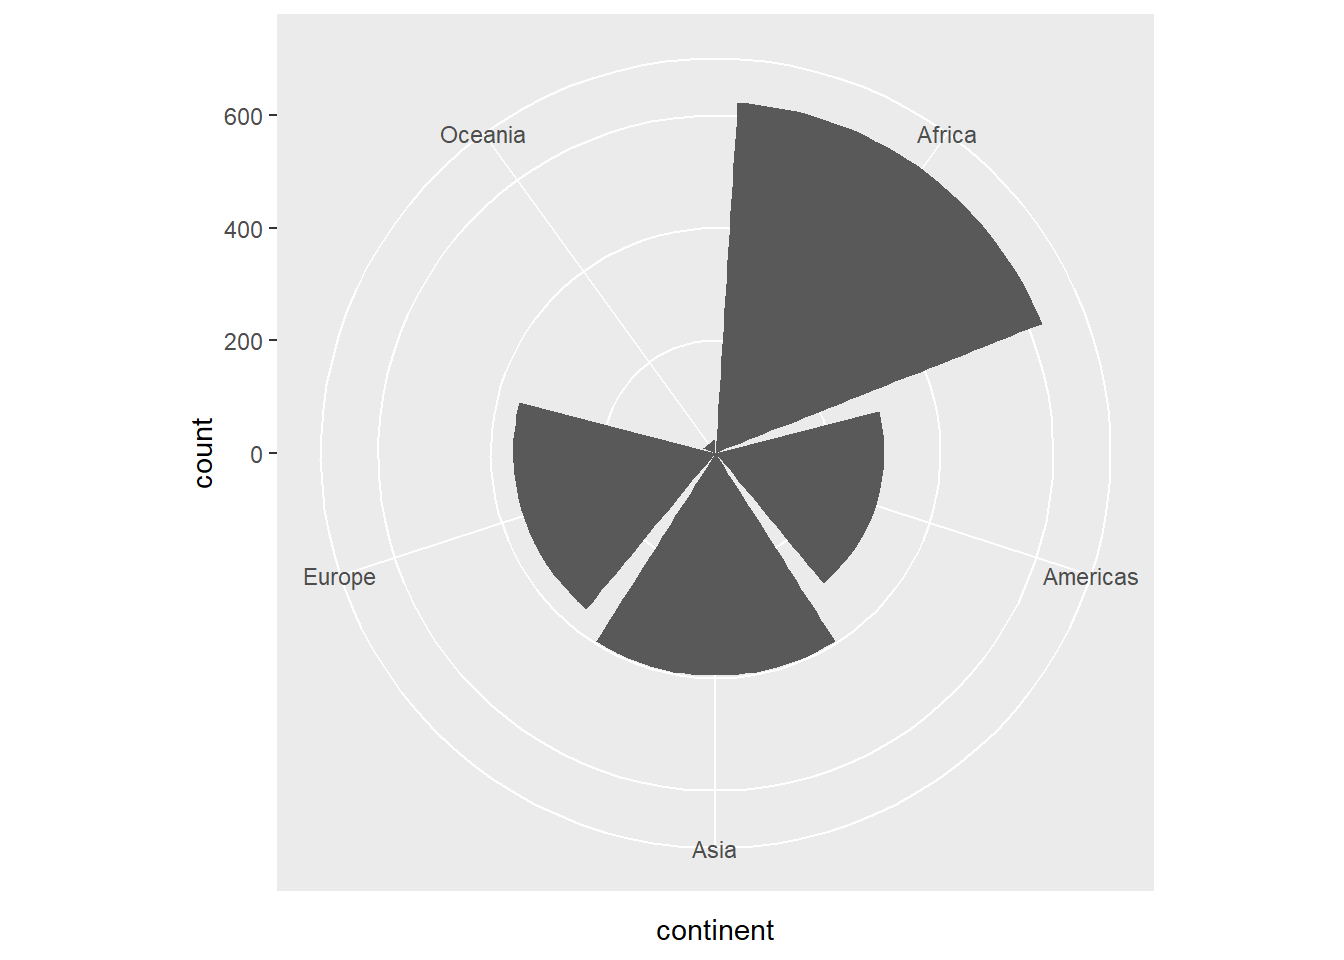
\includegraphics{Applied-Spatial-Data-Analysis_files/figure-latex/unnamed-chunk-5-1.pdf}

\hypertarget{cluster-data-points}{%
\subsubsection{Cluster Data Points}\label{cluster-data-points}}

\begin{Shaded}
\begin{Highlighting}[]
\NormalTok{cluster <-}\StringTok{ }\KeywordTok{read.csv}\NormalTok{(}\StringTok{"C:/Users/01438475/Google Drive/UCTcourses/ASDA/cluster.csv"}\NormalTok{)}
\NormalTok{xy_cluster <-}\StringTok{ }\KeywordTok{matrix}\NormalTok{(}\KeywordTok{cbind}\NormalTok{(cluster}\OperatorTok{$}\NormalTok{X,cluster}\OperatorTok{$}\NormalTok{Y), }\DataTypeTok{ncol=}\DecValTok{2}\NormalTok{)}
\NormalTok{pp_cluster <-}\StringTok{ }\KeywordTok{as.ppp}\NormalTok{(xy_cluster, }\KeywordTok{c}\NormalTok{(}\DecValTok{0}\NormalTok{,}\DecValTok{1}\NormalTok{,}\DecValTok{0}\NormalTok{,}\DecValTok{1}\NormalTok{))}
\KeywordTok{plot}\NormalTok{(pp_cluster)}
\end{Highlighting}
\end{Shaded}

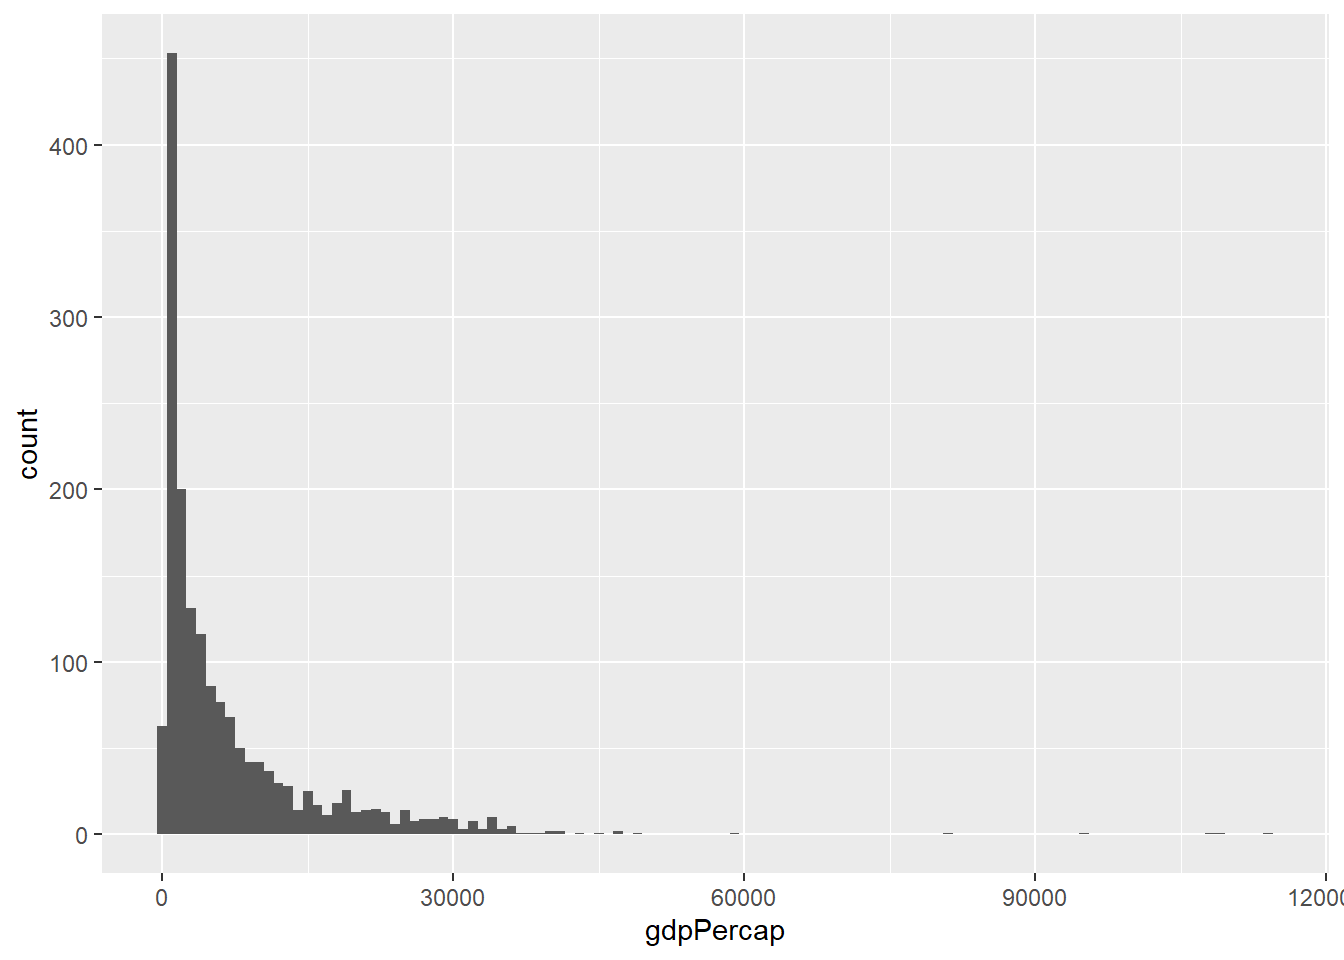
\includegraphics{Applied-Spatial-Data-Analysis_files/figure-latex/unnamed-chunk-6-1.pdf}

\hypertarget{plotting-datasets}{%
\section{Plotting Datasets}\label{plotting-datasets}}

\hypertarget{basic-plot-function}{%
\subsection{Basic plot() function}\label{basic-plot-function}}

\begin{Shaded}
\begin{Highlighting}[]
\KeywordTok{plot}\NormalTok{(swp)}
\end{Highlighting}
\end{Shaded}

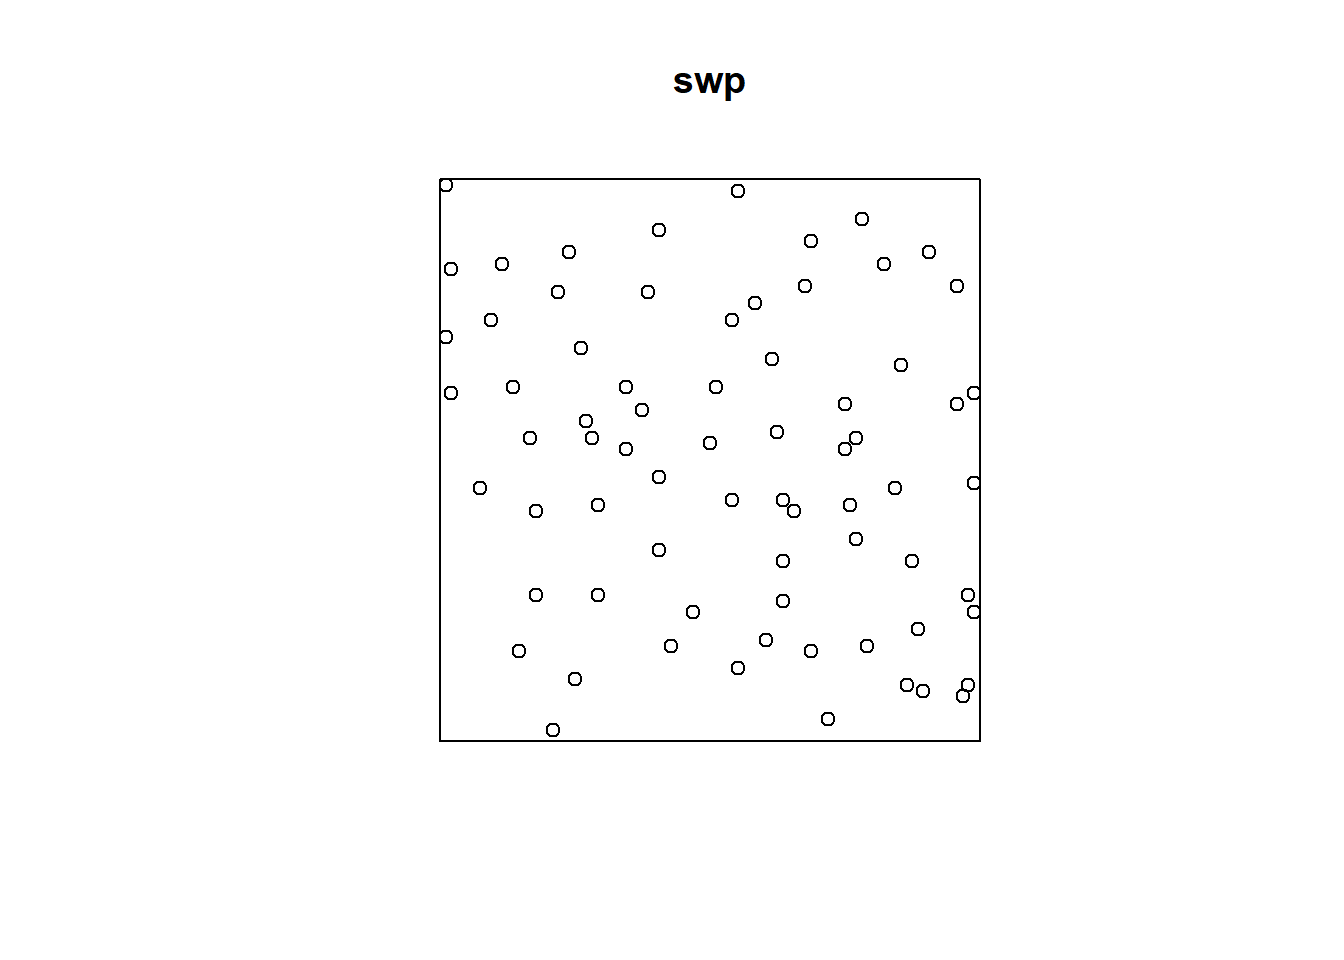
\includegraphics{Applied-Spatial-Data-Analysis_files/figure-latex/unnamed-chunk-7-1.pdf}

\hypertarget{basic-ggplot-function---sf-object}{%
\subsection{Basic ggplot() function - (sf) object}\label{basic-ggplot-function---sf-object}}

\begin{Shaded}
\begin{Highlighting}[]
\KeywordTok{library}\NormalTok{(ggplot2)}
\NormalTok{plot1 =}\StringTok{ }\KeywordTok{ggplot}\NormalTok{() }\OperatorTok{+}\StringTok{ }
\StringTok{  }\KeywordTok{geom_sf}\NormalTok{(}\DataTypeTok{data =}\NormalTok{ clinics_sf, }\DataTypeTok{size =} \FloatTok{.8}\NormalTok{, }\DataTypeTok{color =} \StringTok{"black"}\NormalTok{) }\OperatorTok{+}\StringTok{ }
\StringTok{  }\KeywordTok{ggtitle}\NormalTok{(}\StringTok{"Location of Cape Town clinics - 2016"}\NormalTok{) }\OperatorTok{+}\StringTok{ }
\StringTok{  }\CommentTok{# not specifying crs here, coord_sf will use the CRS defined in the first layer = "+proj=longlat +datum=WGS84 +no_defs"}
\StringTok{  }\KeywordTok{coord_sf}\NormalTok{() }
\NormalTok{plot1}
\end{Highlighting}
\end{Shaded}

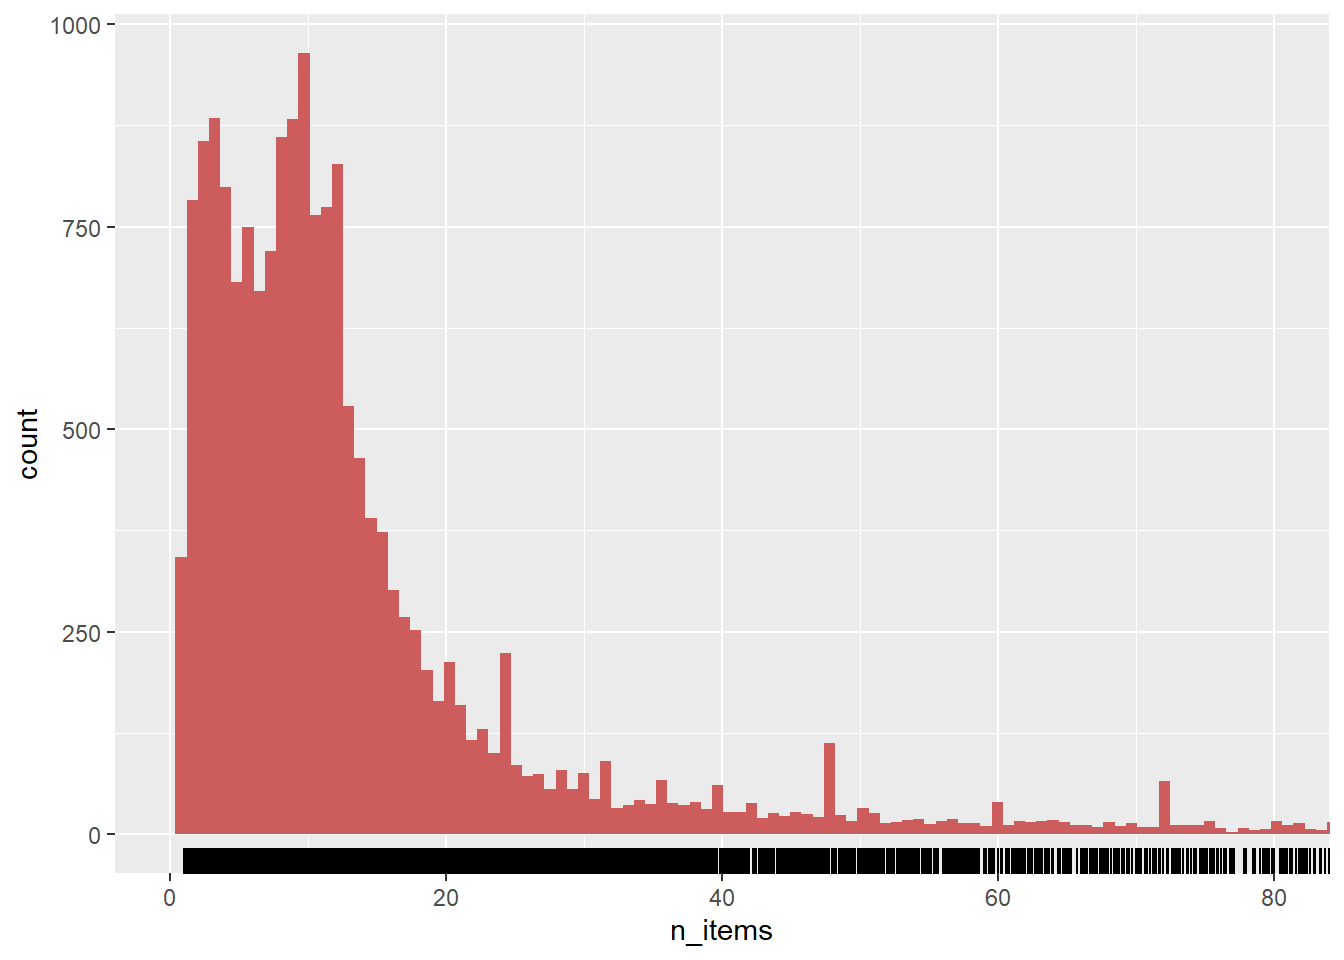
\includegraphics{Applied-Spatial-Data-Analysis_files/figure-latex/unnamed-chunk-8-1.pdf}

\hypertarget{ggplot-function-with-a-bounding-box---sf-object}{%
\subsection{ggplot() function with a bounding box - (sf) object}\label{ggplot-function-with-a-bounding-box---sf-object}}

\begin{Shaded}
\begin{Highlighting}[]
\KeywordTok{library}\NormalTok{(ggplot2)}
\NormalTok{plot2 =}\StringTok{ }\KeywordTok{ggplot}\NormalTok{() }\OperatorTok{+}\StringTok{ }
\StringTok{  }\KeywordTok{geom_sf}\NormalTok{(}\DataTypeTok{data =}\NormalTok{ clinics_sf, }\DataTypeTok{size =} \FloatTok{.8}\NormalTok{, }\DataTypeTok{color =} \StringTok{"black"}\NormalTok{) }\OperatorTok{+}\StringTok{ }
\StringTok{  }\KeywordTok{ggtitle}\NormalTok{(}\StringTok{"Location of Cape Town clinics - 2016"}\NormalTok{) }\OperatorTok{+}\StringTok{ }
\StringTok{  }\KeywordTok{coord_sf}\NormalTok{(}\DataTypeTok{xlim =} \KeywordTok{c}\NormalTok{(}\FloatTok{18.34}\NormalTok{, }\FloatTok{18.91}\NormalTok{), }\DataTypeTok{ylim =} \KeywordTok{c}\NormalTok{(}\OperatorTok{-}\FloatTok{34.19}\NormalTok{, }\FloatTok{-33.51262}\NormalTok{)) }\OperatorTok{+}
\StringTok{  }\KeywordTok{theme}\NormalTok{(}\DataTypeTok{panel.grid.major =} \KeywordTok{element_blank}\NormalTok{(), }
        \DataTypeTok{panel.grid.minor =} \KeywordTok{element_blank}\NormalTok{(),}
        \DataTypeTok{panel.background =} \KeywordTok{element_rect}\NormalTok{(}\DataTypeTok{colour =} \StringTok{"black"}\NormalTok{, }\DataTypeTok{size=}\DecValTok{1}\NormalTok{, }\DataTypeTok{fill=}\OtherTok{NA}\NormalTok{))}
\NormalTok{plot2}
\end{Highlighting}
\end{Shaded}

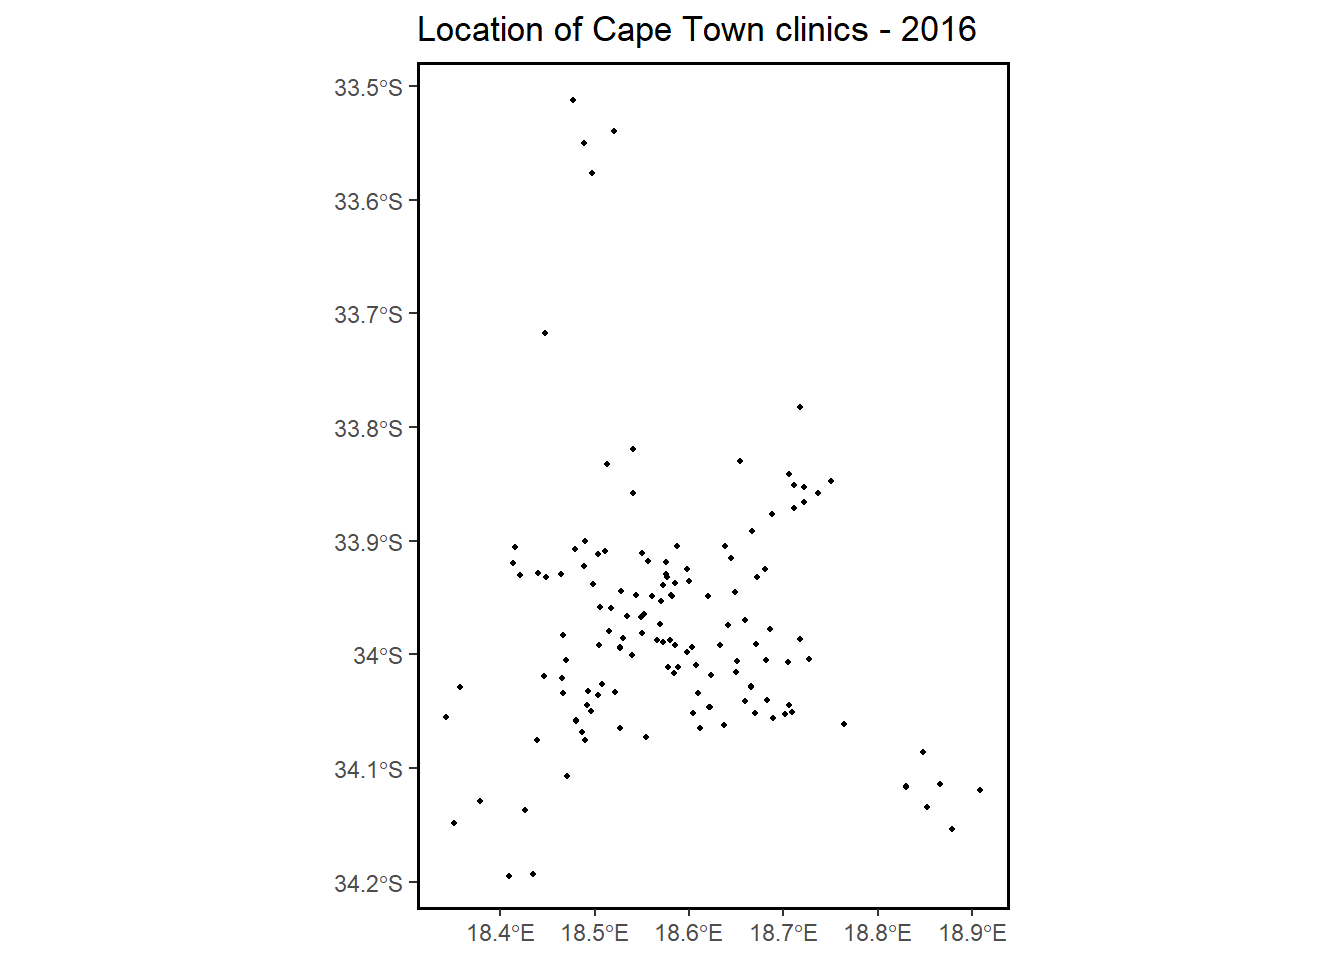
\includegraphics{Applied-Spatial-Data-Analysis_files/figure-latex/unnamed-chunk-9-1.pdf}

\hypertarget{ggplot-with-electoral-wards-shape-file}{%
\subsection{ggplot() with Electoral Wards Shape File}\label{ggplot-with-electoral-wards-shape-file}}

In order to plot using the electoral wards polygons, we need the sf data frame to be converted into Spatial Points Data Frame (sp).

\begin{Shaded}
\begin{Highlighting}[]
\NormalTok{clinics_sp <-}\StringTok{ }\KeywordTok{as}\NormalTok{(clinics_sf, }\DataTypeTok{Class =} \StringTok{"Spatial"}\NormalTok{)}
\KeywordTok{class}\NormalTok{(clinics_sp)}
\end{Highlighting}
\end{Shaded}

\begin{verbatim}
## [1] "SpatialPointsDataFrame"
## attr(,"package")
## [1] "sp"
\end{verbatim}

Download the CPT electoral wards and import the shape file as follows:

\begin{Shaded}
\begin{Highlighting}[]
\KeywordTok{library}\NormalTok{(sf)}
\NormalTok{ct.wards_sf =}\StringTok{ }\KeywordTok{st_read}\NormalTok{(}\StringTok{"C:/Users/01438475/Google Drive/UCTcourses/ASDA/DataSets/sa/CPT/electoral wards for cpt.shp"}\NormalTok{)}
\end{Highlighting}
\end{Shaded}

\begin{verbatim}
## Reading layer `electoral wards for cpt' from data source `C:\Users\01438475\Google Drive\UCTcourses\ASDA\DataSets\sa\CPT\electoral wards for cpt.shp' using driver `ESRI Shapefile'
## Simple feature collection with 111 features and 9 fields
## geometry type:  MULTIPOLYGON
## dimension:      XY
## bbox:           xmin: 18.30722 ymin: -34.35834 xmax: 19.00467 ymax: -33.47128
## CRS:            NA
\end{verbatim}

\begin{Shaded}
\begin{Highlighting}[]
\KeywordTok{st_geometry_type}\NormalTok{(ct.wards_sf)}
\end{Highlighting}
\end{Shaded}

\begin{verbatim}
##   [1] MULTIPOLYGON MULTIPOLYGON MULTIPOLYGON MULTIPOLYGON MULTIPOLYGON
##   [6] MULTIPOLYGON MULTIPOLYGON MULTIPOLYGON MULTIPOLYGON MULTIPOLYGON
##  [11] MULTIPOLYGON MULTIPOLYGON MULTIPOLYGON MULTIPOLYGON MULTIPOLYGON
##  [16] MULTIPOLYGON MULTIPOLYGON MULTIPOLYGON MULTIPOLYGON MULTIPOLYGON
##  [21] MULTIPOLYGON MULTIPOLYGON MULTIPOLYGON MULTIPOLYGON MULTIPOLYGON
##  [26] MULTIPOLYGON MULTIPOLYGON MULTIPOLYGON MULTIPOLYGON MULTIPOLYGON
##  [31] MULTIPOLYGON MULTIPOLYGON MULTIPOLYGON MULTIPOLYGON MULTIPOLYGON
##  [36] MULTIPOLYGON MULTIPOLYGON MULTIPOLYGON MULTIPOLYGON MULTIPOLYGON
##  [41] MULTIPOLYGON MULTIPOLYGON MULTIPOLYGON MULTIPOLYGON MULTIPOLYGON
##  [46] MULTIPOLYGON MULTIPOLYGON MULTIPOLYGON MULTIPOLYGON MULTIPOLYGON
##  [51] MULTIPOLYGON MULTIPOLYGON MULTIPOLYGON MULTIPOLYGON MULTIPOLYGON
##  [56] MULTIPOLYGON MULTIPOLYGON MULTIPOLYGON MULTIPOLYGON MULTIPOLYGON
##  [61] MULTIPOLYGON MULTIPOLYGON MULTIPOLYGON MULTIPOLYGON MULTIPOLYGON
##  [66] MULTIPOLYGON MULTIPOLYGON MULTIPOLYGON MULTIPOLYGON MULTIPOLYGON
##  [71] MULTIPOLYGON MULTIPOLYGON MULTIPOLYGON MULTIPOLYGON MULTIPOLYGON
##  [76] MULTIPOLYGON MULTIPOLYGON MULTIPOLYGON MULTIPOLYGON MULTIPOLYGON
##  [81] MULTIPOLYGON MULTIPOLYGON MULTIPOLYGON MULTIPOLYGON MULTIPOLYGON
##  [86] MULTIPOLYGON MULTIPOLYGON MULTIPOLYGON MULTIPOLYGON MULTIPOLYGON
##  [91] MULTIPOLYGON MULTIPOLYGON MULTIPOLYGON MULTIPOLYGON MULTIPOLYGON
##  [96] MULTIPOLYGON MULTIPOLYGON MULTIPOLYGON MULTIPOLYGON MULTIPOLYGON
## [101] MULTIPOLYGON MULTIPOLYGON MULTIPOLYGON MULTIPOLYGON MULTIPOLYGON
## [106] MULTIPOLYGON MULTIPOLYGON MULTIPOLYGON MULTIPOLYGON MULTIPOLYGON
## [111] MULTIPOLYGON
## 18 Levels: GEOMETRY POINT LINESTRING POLYGON MULTIPOINT ... TRIANGLE
\end{verbatim}

\begin{Shaded}
\begin{Highlighting}[]
\KeywordTok{library}\NormalTok{(ggplot2)}
\KeywordTok{ggplot}\NormalTok{() }\OperatorTok{+}\StringTok{ }
\StringTok{  }\KeywordTok{geom_sf}\NormalTok{(}\DataTypeTok{data =}\NormalTok{ ct.wards_sf, }\DataTypeTok{size =} \FloatTok{.5}\NormalTok{, }\DataTypeTok{color =} \StringTok{"black"}\NormalTok{) }\OperatorTok{+}\StringTok{ }
\StringTok{  }\KeywordTok{geom_point}\NormalTok{(}\KeywordTok{aes}\NormalTok{(}\DataTypeTok{x =}\NormalTok{ clinics_sp}\OperatorTok{@}\NormalTok{coords[,}\DecValTok{1}\NormalTok{], }\DataTypeTok{y =}\NormalTok{ clinics_sp}\OperatorTok{@}\NormalTok{coords[,}\DecValTok{2}\NormalTok{]),}
             \DataTypeTok{data =}\NormalTok{ clinics_sp}\OperatorTok{@}\NormalTok{data, }\DataTypeTok{alpha =} \DecValTok{1}\NormalTok{,}\DataTypeTok{size=}\DecValTok{2}\NormalTok{, }\DataTypeTok{color =} \StringTok{"red"}\NormalTok{)}\OperatorTok{+}\StringTok{ }
\StringTok{  }\KeywordTok{ggtitle}\NormalTok{(}\StringTok{"Spatial locations of Cape Town clinics within wards"}\NormalTok{) }\OperatorTok{+}\StringTok{ }
\StringTok{  }\KeywordTok{coord_sf}\NormalTok{()}
\end{Highlighting}
\end{Shaded}

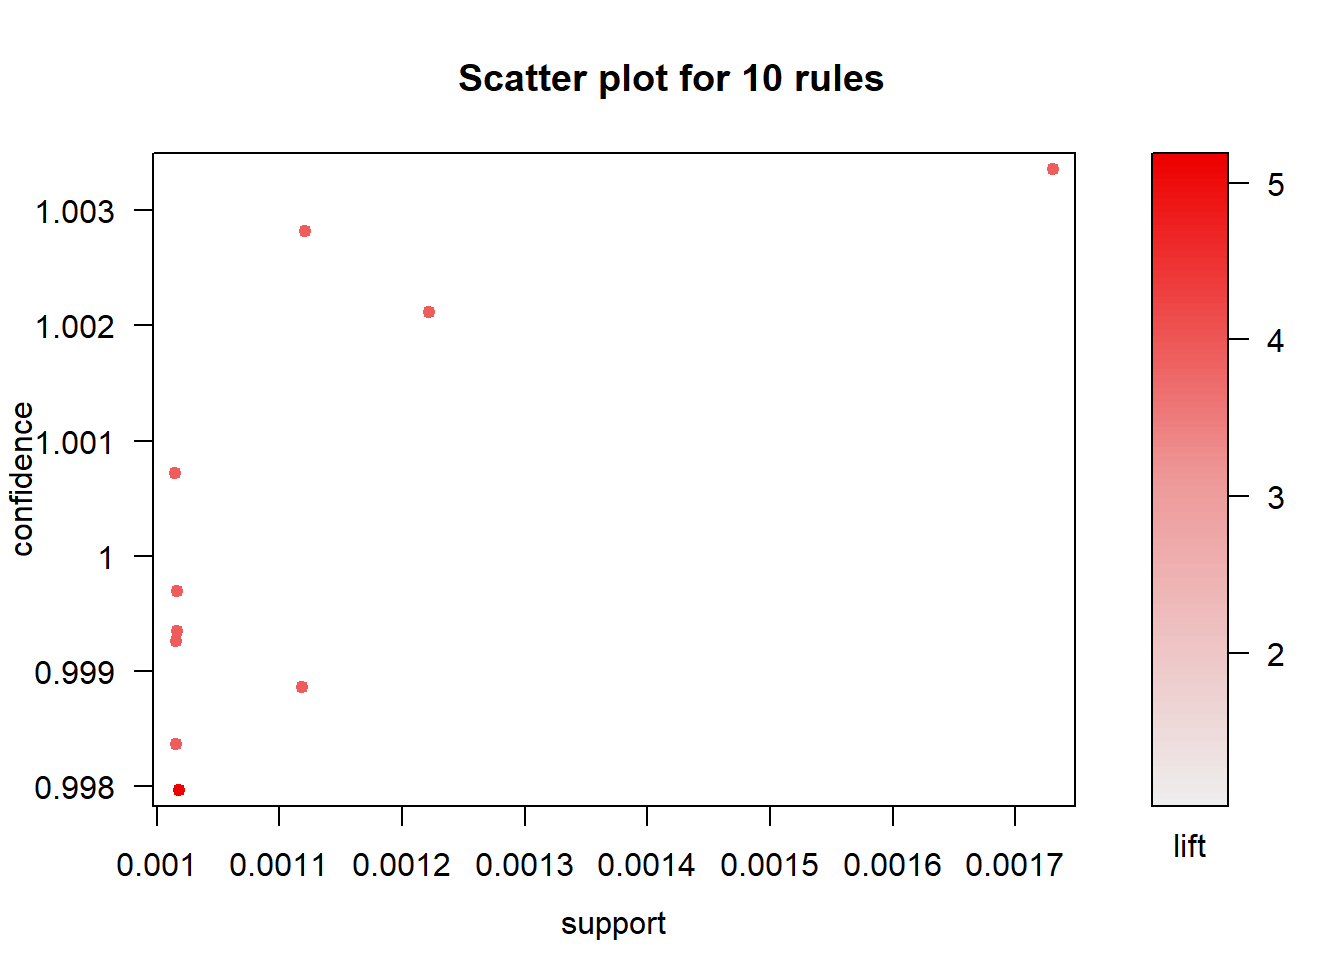
\includegraphics{Applied-Spatial-Data-Analysis_files/figure-latex/unnamed-chunk-11-1.pdf}

\hypertarget{plotting-with-google-maps}{%
\subsection{Plotting with google maps:}\label{plotting-with-google-maps}}

\begin{Shaded}
\begin{Highlighting}[]
\KeywordTok{require}\NormalTok{(}\StringTok{"maps"}\NormalTok{)}
\KeywordTok{require}\NormalTok{(}\StringTok{"ggplot2"}\NormalTok{)}
\end{Highlighting}
\end{Shaded}

First specify the outer boundaries of Google Map

\begin{Shaded}
\begin{Highlighting}[]
\KeywordTok{require}\NormalTok{(}\StringTok{"ggmap"}\NormalTok{)}
\NormalTok{caLongLat <-}\KeywordTok{c}\NormalTok{(}\KeywordTok{bbox}\NormalTok{(clinics_sp)[}\DecValTok{1}\NormalTok{,}\DecValTok{1}\NormalTok{], }\KeywordTok{bbox}\NormalTok{(clinics_sp)[}\DecValTok{2}\NormalTok{,}\DecValTok{1}\NormalTok{], }\KeywordTok{bbox}\NormalTok{(clinics_sp)[}\DecValTok{1}\NormalTok{,}\DecValTok{2}\NormalTok{],}\KeywordTok{bbox}\NormalTok{(clinics_sp)[}\DecValTok{2}\NormalTok{,}\DecValTok{2}\NormalTok{])}
\NormalTok{caLongLat}
\end{Highlighting}
\end{Shaded}

\begin{verbatim}
## [1]  18.34268 -34.19491  18.90847 -33.51262
\end{verbatim}

\begin{Shaded}
\begin{Highlighting}[]
\NormalTok{caLongLat<-}\KeywordTok{c}\NormalTok{(}\DecValTok{18}\NormalTok{, }\FloatTok{-34.3}\NormalTok{,  }\DecValTok{19}\NormalTok{, }\FloatTok{-33.2}\NormalTok{)}
\NormalTok{map <-}\StringTok{ }\KeywordTok{get_map}\NormalTok{(}\DataTypeTok{location =}\NormalTok{ caLongLat)}
\end{Highlighting}
\end{Shaded}

Google Map Plot

\begin{Shaded}
\begin{Highlighting}[]
\NormalTok{mapPoints <-}\StringTok{ }\KeywordTok{ggmap}\NormalTok{(map) }\OperatorTok{+}\StringTok{ }
\StringTok{  }\KeywordTok{geom_point}\NormalTok{(}\KeywordTok{aes}\NormalTok{(}\DataTypeTok{x =}\NormalTok{ clinics_sp}\OperatorTok{@}\NormalTok{coords[,}\DecValTok{1}\NormalTok{], }\DataTypeTok{y =}\NormalTok{ clinics_sp}\OperatorTok{@}\NormalTok{coords[,}\DecValTok{2}\NormalTok{]),}
             \DataTypeTok{data =}\NormalTok{ clinics_sp}\OperatorTok{@}\NormalTok{data, }\DataTypeTok{alpha =} \FloatTok{0.7}\NormalTok{,}\DataTypeTok{size=}\DecValTok{2}\NormalTok{)}\OperatorTok{+}\StringTok{ }
\StringTok{  }\KeywordTok{labs}\NormalTok{(}\DataTypeTok{title=}\StringTok{"Spatial location of clinics"}\NormalTok{,}
       \DataTypeTok{y=}\StringTok{"Latitude"}\NormalTok{,}\DataTypeTok{x=}\StringTok{"Longtitude"}\NormalTok{ )}

\NormalTok{mapPoints}
\end{Highlighting}
\end{Shaded}

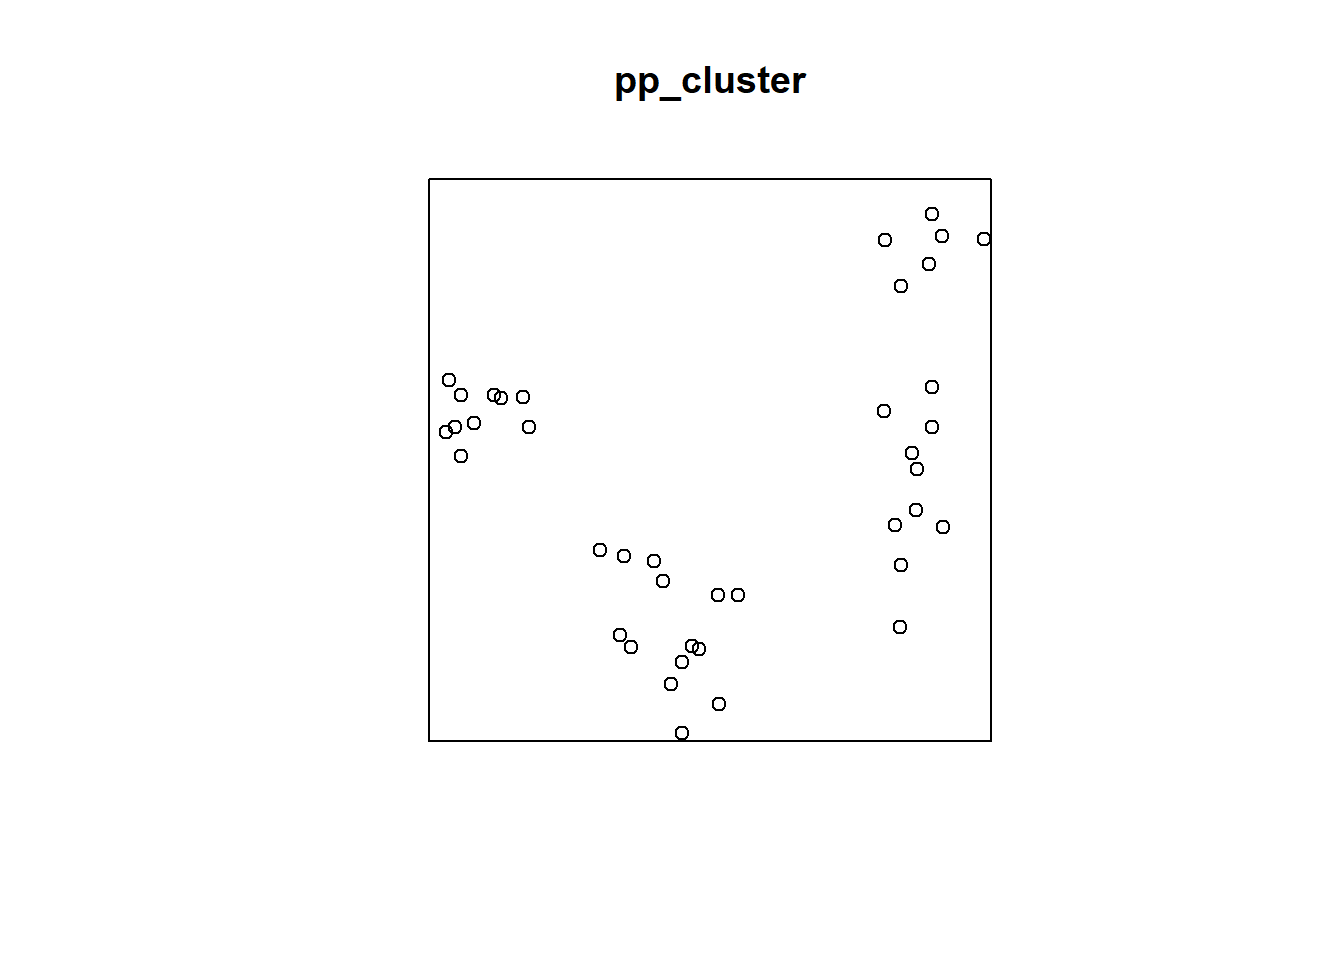
\includegraphics{Applied-Spatial-Data-Analysis_files/figure-latex/unnamed-chunk-14-1.pdf}

\hypertarget{quadrat-analysis---quadrat-counts-and-tests}{%
\section{Quadrat Analysis - Quadrat Counts and Tests}\label{quadrat-analysis---quadrat-counts-and-tests}}

\hypertarget{swp-dataset}{%
\subsection{swp dataset}\label{swp-dataset}}

Quadrat counts:

\begin{Shaded}
\begin{Highlighting}[]
\NormalTok{Q3x3 =}\StringTok{ }\KeywordTok{quadratcount}\NormalTok{(swp, }\DataTypeTok{nx=}\DecValTok{3}\NormalTok{, }\DataTypeTok{ny=}\DecValTok{3}\NormalTok{)}
\KeywordTok{plot}\NormalTok{(swp)}
\KeywordTok{plot}\NormalTok{(Q3x3, }\DataTypeTok{add=}\OtherTok{TRUE}\NormalTok{, }\DataTypeTok{col=}\StringTok{"red"}\NormalTok{, }\DataTypeTok{cex=}\FloatTok{1.5}\NormalTok{, }\DataTypeTok{lty=}\DecValTok{2}\NormalTok{)}
\end{Highlighting}
\end{Shaded}

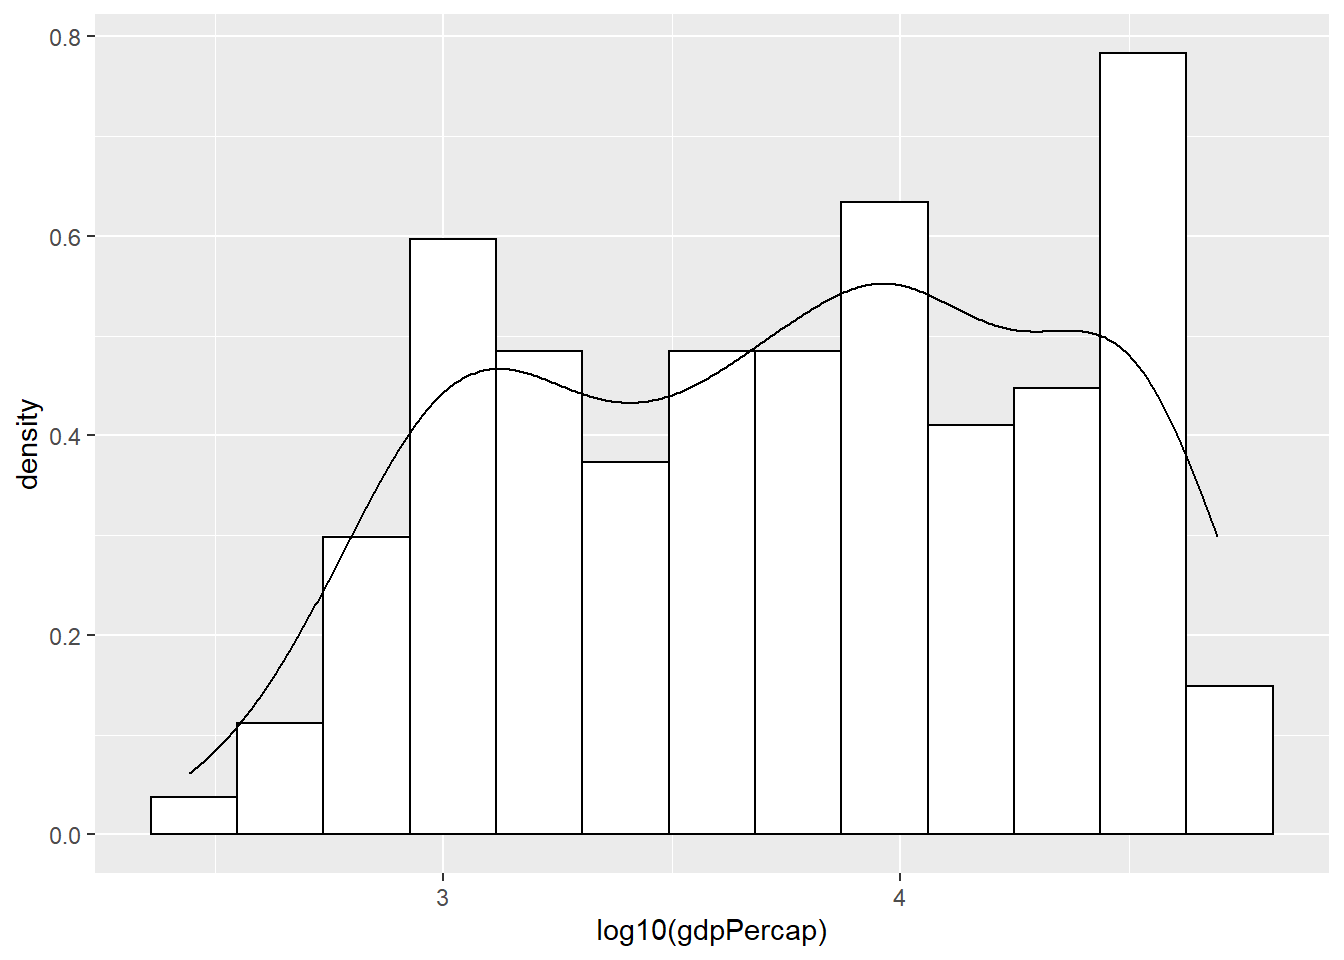
\includegraphics{Applied-Spatial-Data-Analysis_files/figure-latex/unnamed-chunk-15-1.pdf}

\begin{Shaded}
\begin{Highlighting}[]
\CommentTok{# Plot the density}
\NormalTok{cl <-}\StringTok{  }\KeywordTok{interp.colours}\NormalTok{(}\KeywordTok{c}\NormalTok{(}\StringTok{"lightyellow"}\NormalTok{, }\StringTok{"orange"}\NormalTok{ ,}\StringTok{"red"}\NormalTok{), }\DecValTok{20}\NormalTok{)}

\KeywordTok{plot}\NormalTok{( }\KeywordTok{intensity}\NormalTok{(Q3x3, }\DataTypeTok{image=}\OtherTok{TRUE}\NormalTok{), }\DataTypeTok{las=}\DecValTok{1}\NormalTok{, }\DataTypeTok{col=}\NormalTok{cl, }\DataTypeTok{main=}\OtherTok{NULL}\NormalTok{)}
\KeywordTok{plot}\NormalTok{(swp, }\DataTypeTok{pch=}\DecValTok{20}\NormalTok{, }\DataTypeTok{cex=}\FloatTok{0.6}\NormalTok{, }\DataTypeTok{col=}\StringTok{"black"}\NormalTok{, }\DataTypeTok{add=}\OtherTok{TRUE}\NormalTok{)  }\CommentTok{# Add points}
\end{Highlighting}
\end{Shaded}

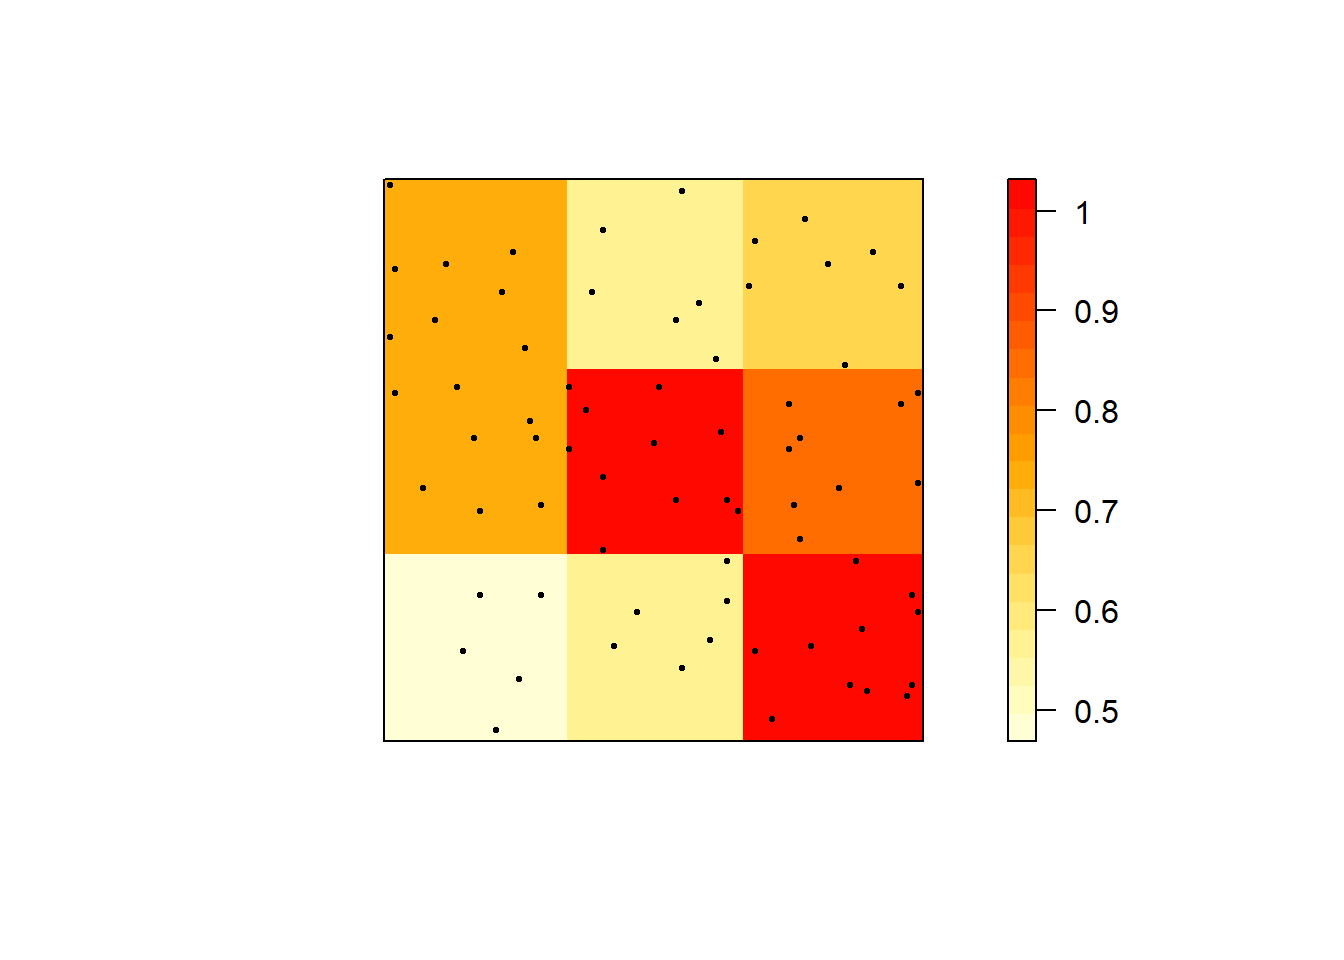
\includegraphics{Applied-Spatial-Data-Analysis_files/figure-latex/unnamed-chunk-15-2.pdf}

Quadrat test

\begin{Shaded}
\begin{Highlighting}[]
\NormalTok{Q3x3test =}\StringTok{ }\KeywordTok{quadrat.test}\NormalTok{(swp, }\DecValTok{3}\NormalTok{,}\DecValTok{3}\NormalTok{)}
\NormalTok{Q3x3test}
\end{Highlighting}
\end{Shaded}

\begin{verbatim}
## 
## 	Chi-squared test of CSR using quadrat counts
## 
## data:  swp
## X2 = 4.6761, df = 8, p-value = 0.4169
## alternative hypothesis: two.sided
## 
## Quadrats: 3 by 3 grid of tiles
\end{verbatim}

\hypertarget{simulated-csr-pattern}{%
\subsection{Simulated CSR Pattern}\label{simulated-csr-pattern}}

\begin{Shaded}
\begin{Highlighting}[]
\NormalTok{Q3x3_csr =}\StringTok{ }\KeywordTok{quadratcount}\NormalTok{(pp_csr, }\DataTypeTok{nx=}\DecValTok{3}\NormalTok{, }\DataTypeTok{ny=}\DecValTok{3}\NormalTok{)}
\KeywordTok{plot}\NormalTok{(pp_csr)}
\KeywordTok{plot}\NormalTok{(Q3x3_csr, }\DataTypeTok{add=}\OtherTok{TRUE}\NormalTok{, }\DataTypeTok{col=}\StringTok{"red"}\NormalTok{, }\DataTypeTok{cex=}\FloatTok{1.5}\NormalTok{, }\DataTypeTok{lty=}\DecValTok{2}\NormalTok{)}
\end{Highlighting}
\end{Shaded}

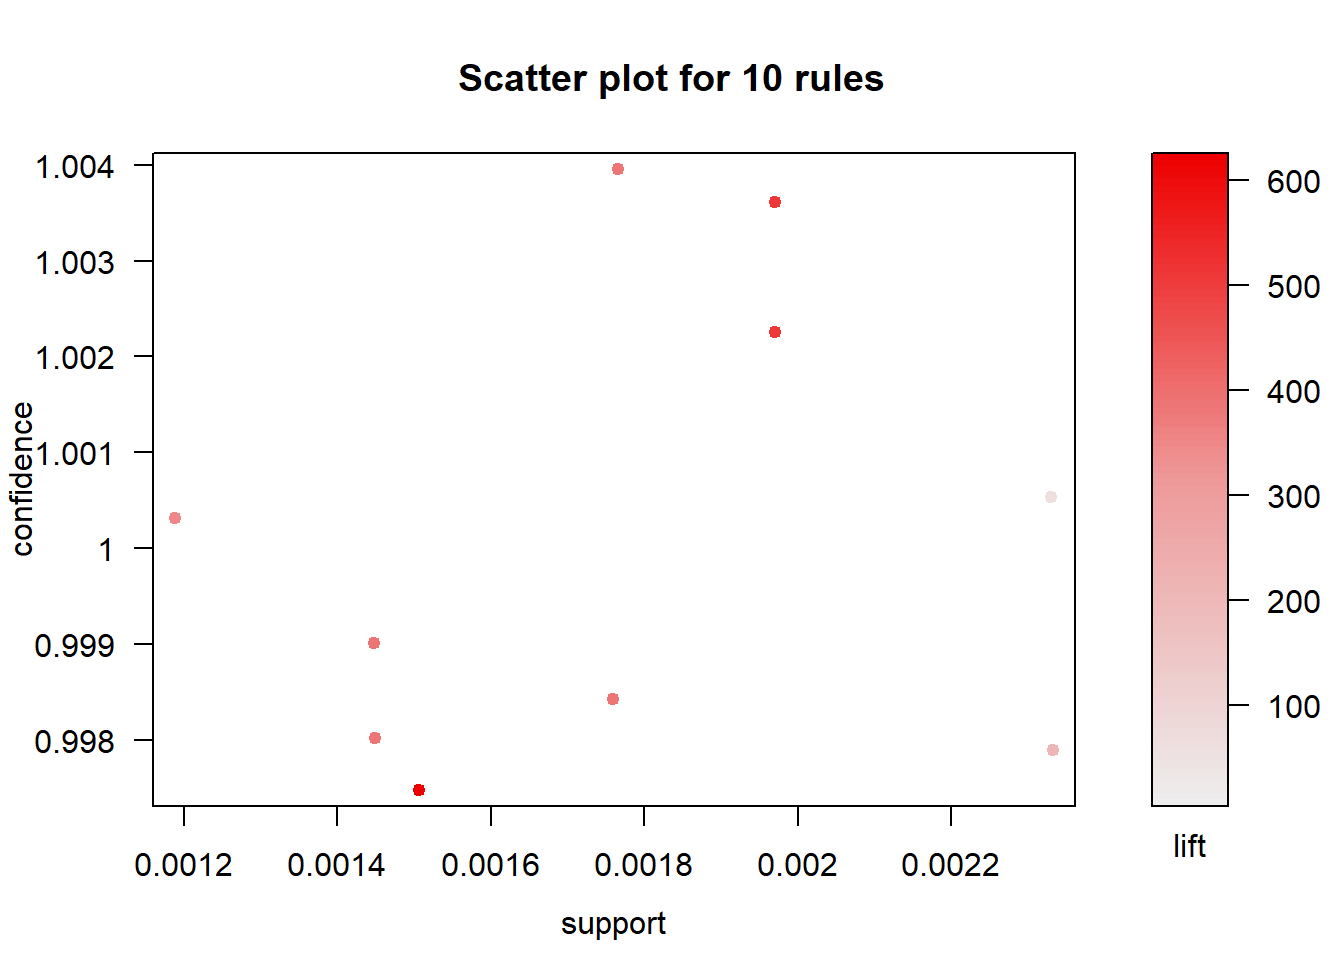
\includegraphics{Applied-Spatial-Data-Analysis_files/figure-latex/unnamed-chunk-17-1.pdf}

Test:

\begin{Shaded}
\begin{Highlighting}[]
\NormalTok{Q3x3test_csr =}\StringTok{ }\KeywordTok{quadrat.test}\NormalTok{(pp_csr, }\DecValTok{3}\NormalTok{,}\DecValTok{3}\NormalTok{)}
\end{Highlighting}
\end{Shaded}

\begin{verbatim}
## Warning: Some expected counts are small; chi^2 approximation may be inaccurate
\end{verbatim}

\begin{Shaded}
\begin{Highlighting}[]
\NormalTok{Q3x3test_csr}
\end{Highlighting}
\end{Shaded}

\begin{verbatim}
## 
## 	Chi-squared test of CSR using quadrat counts
## 
## data:  pp_csr
## X2 = 11.3, df = 8, p-value = 0.3705
## alternative hypothesis: two.sided
## 
## Quadrats: 3 by 3 grid of tiles
\end{verbatim}

\hypertarget{simulated-cluster-pattern}{%
\subsection{Simulated Cluster Pattern}\label{simulated-cluster-pattern}}

\begin{Shaded}
\begin{Highlighting}[]
\NormalTok{Q3x3_cluster =}\StringTok{ }\KeywordTok{quadratcount}\NormalTok{(pp_cluster, }\DataTypeTok{nx=}\DecValTok{3}\NormalTok{, }\DataTypeTok{ny=}\DecValTok{3}\NormalTok{)}
\KeywordTok{plot}\NormalTok{(pp_cluster)}
\KeywordTok{plot}\NormalTok{(Q3x3_cluster, }\DataTypeTok{add=}\OtherTok{TRUE}\NormalTok{, }\DataTypeTok{col=}\StringTok{"red"}\NormalTok{, }\DataTypeTok{cex=}\FloatTok{1.5}\NormalTok{, }\DataTypeTok{lty=}\DecValTok{2}\NormalTok{)}
\end{Highlighting}
\end{Shaded}

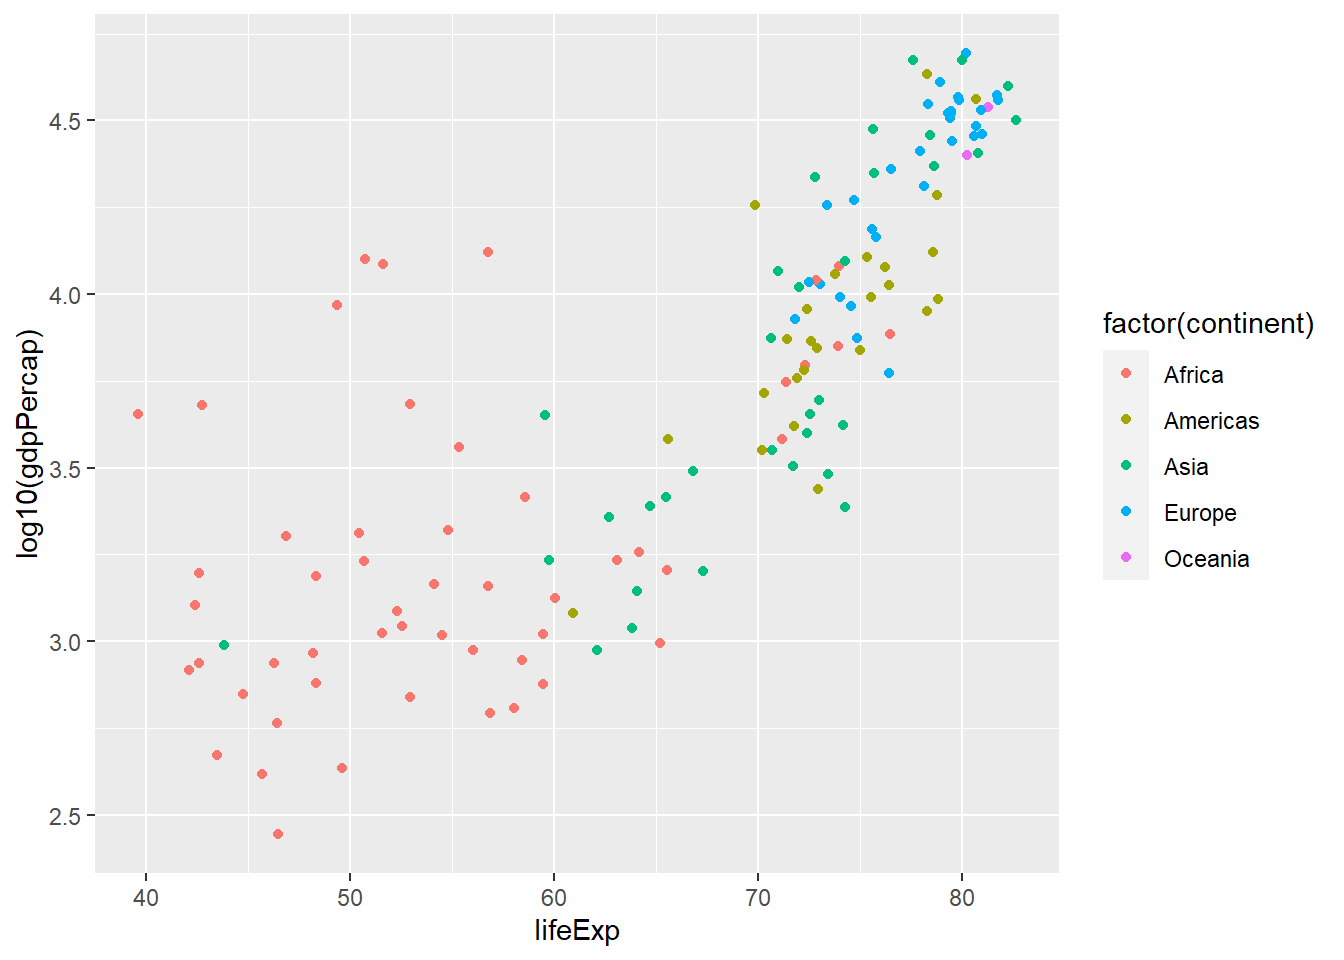
\includegraphics{Applied-Spatial-Data-Analysis_files/figure-latex/unnamed-chunk-19-1.pdf}

Test:

\begin{Shaded}
\begin{Highlighting}[]
\NormalTok{Q3x3test_cluster =}\StringTok{ }\KeywordTok{quadrat.test}\NormalTok{(pp_cluster, }\DecValTok{3}\NormalTok{,}\DecValTok{3}\NormalTok{)}
\end{Highlighting}
\end{Shaded}

\begin{verbatim}
## Warning: Some expected counts are small; chi^2 approximation may be inaccurate
\end{verbatim}

\begin{Shaded}
\begin{Highlighting}[]
\NormalTok{Q3x3test_cluster}
\end{Highlighting}
\end{Shaded}

\begin{verbatim}
## 
## 	Chi-squared test of CSR using quadrat counts
## 
## data:  pp_cluster
## X2 = 48.65, df = 8, p-value = 1.484e-07
## alternative hypothesis: two.sided
## 
## Quadrats: 3 by 3 grid of tiles
\end{verbatim}

\hypertarget{simulated-regular-pattern}{%
\subsection{Simulated Regular Pattern}\label{simulated-regular-pattern}}

\begin{Shaded}
\begin{Highlighting}[]
\NormalTok{Q3x3_regular =}\StringTok{ }\KeywordTok{quadratcount}\NormalTok{(pp_regular, }\DataTypeTok{nx=}\DecValTok{4}\NormalTok{, }\DataTypeTok{ny=}\DecValTok{4}\NormalTok{)}
\KeywordTok{plot}\NormalTok{(pp_regular)}
\KeywordTok{plot}\NormalTok{(Q3x3_regular, }\DataTypeTok{add=}\OtherTok{TRUE}\NormalTok{, }\DataTypeTok{col=}\StringTok{"red"}\NormalTok{, }\DataTypeTok{cex=}\FloatTok{1.5}\NormalTok{, }\DataTypeTok{lty=}\DecValTok{2}\NormalTok{)}
\end{Highlighting}
\end{Shaded}

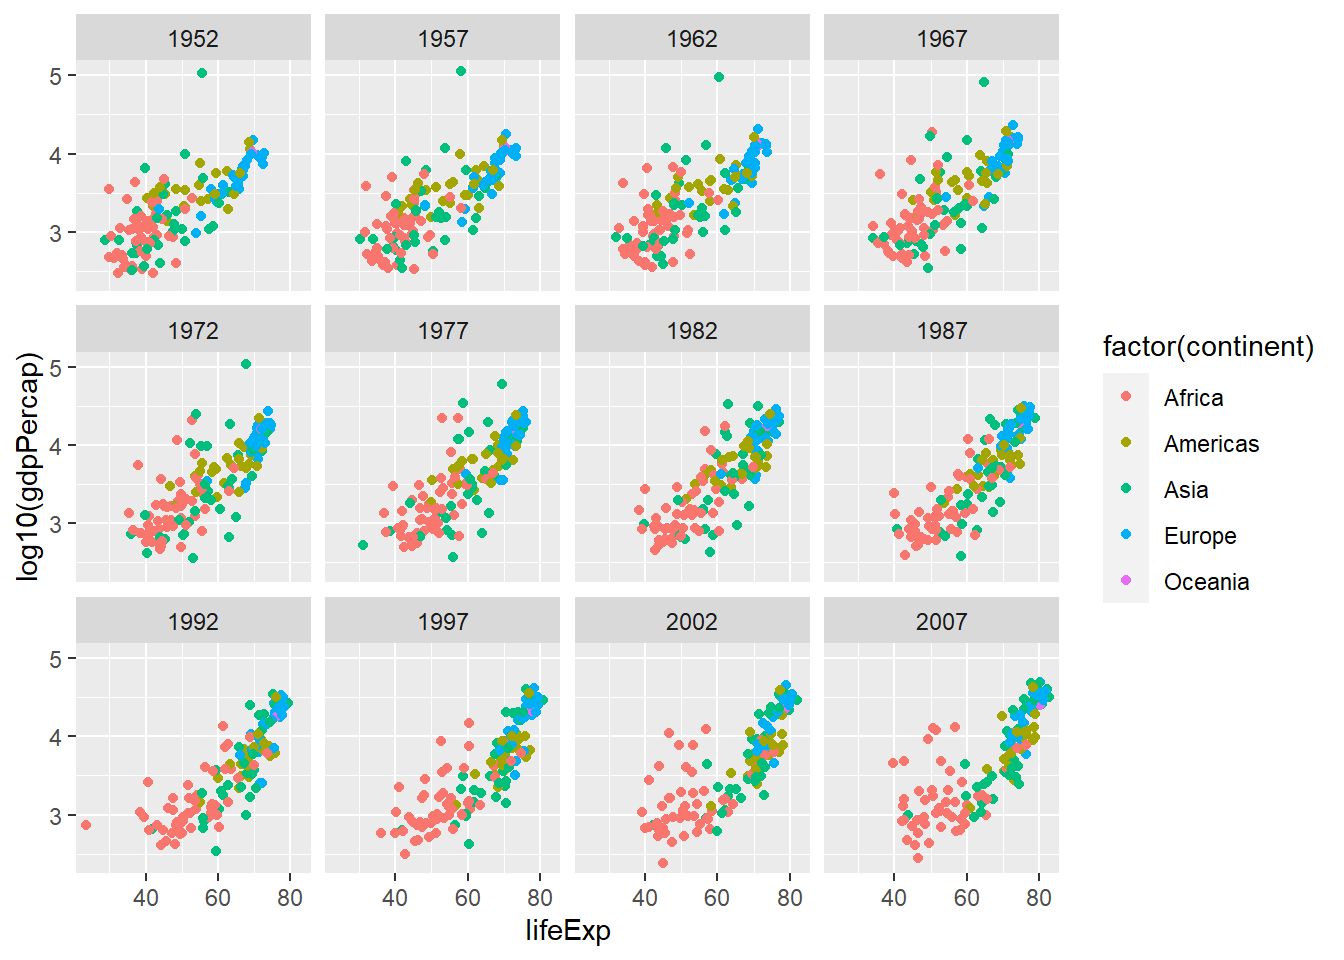
\includegraphics{Applied-Spatial-Data-Analysis_files/figure-latex/unnamed-chunk-21-1.pdf}

Test:

\begin{Shaded}
\begin{Highlighting}[]
\NormalTok{Q3x3test_regular =}\StringTok{ }\KeywordTok{quadrat.test}\NormalTok{(pp_regular, }\DecValTok{3}\NormalTok{,}\DecValTok{3}\NormalTok{)}
\end{Highlighting}
\end{Shaded}

\begin{verbatim}
## Warning: Some expected counts are small; chi^2 approximation may be inaccurate
\end{verbatim}

\begin{Shaded}
\begin{Highlighting}[]
\NormalTok{Q3x3test_regular}
\end{Highlighting}
\end{Shaded}

\begin{verbatim}
## 
## 	Chi-squared test of CSR using quadrat counts
## 
## data:  pp_regular
## X2 = 4.55, df = 8, p-value = 0.3912
## alternative hypothesis: two.sided
## 
## Quadrats: 3 by 3 grid of tiles
\end{verbatim}

\hypertarget{kernel-density-smoothing}{%
\section{Kernel Density Smoothing}\label{kernel-density-smoothing}}

\hypertarget{csr-pattern}{%
\subsection{CSR Pattern}\label{csr-pattern}}

\begin{Shaded}
\begin{Highlighting}[]
\NormalTok{den <-}\StringTok{ }\KeywordTok{density}\NormalTok{(pp_csr, }\DataTypeTok{sigma =} \FloatTok{.1}\NormalTok{)}
\KeywordTok{plot}\NormalTok{(den, }\DataTypeTok{main =} \StringTok{"CSR"}\NormalTok{)}
\KeywordTok{plot}\NormalTok{(pp_csr, }\DataTypeTok{add=}\OtherTok{TRUE}\NormalTok{)}
\KeywordTok{contour}\NormalTok{(den, }\DataTypeTok{add =} \OtherTok{TRUE}\NormalTok{)}
\end{Highlighting}
\end{Shaded}

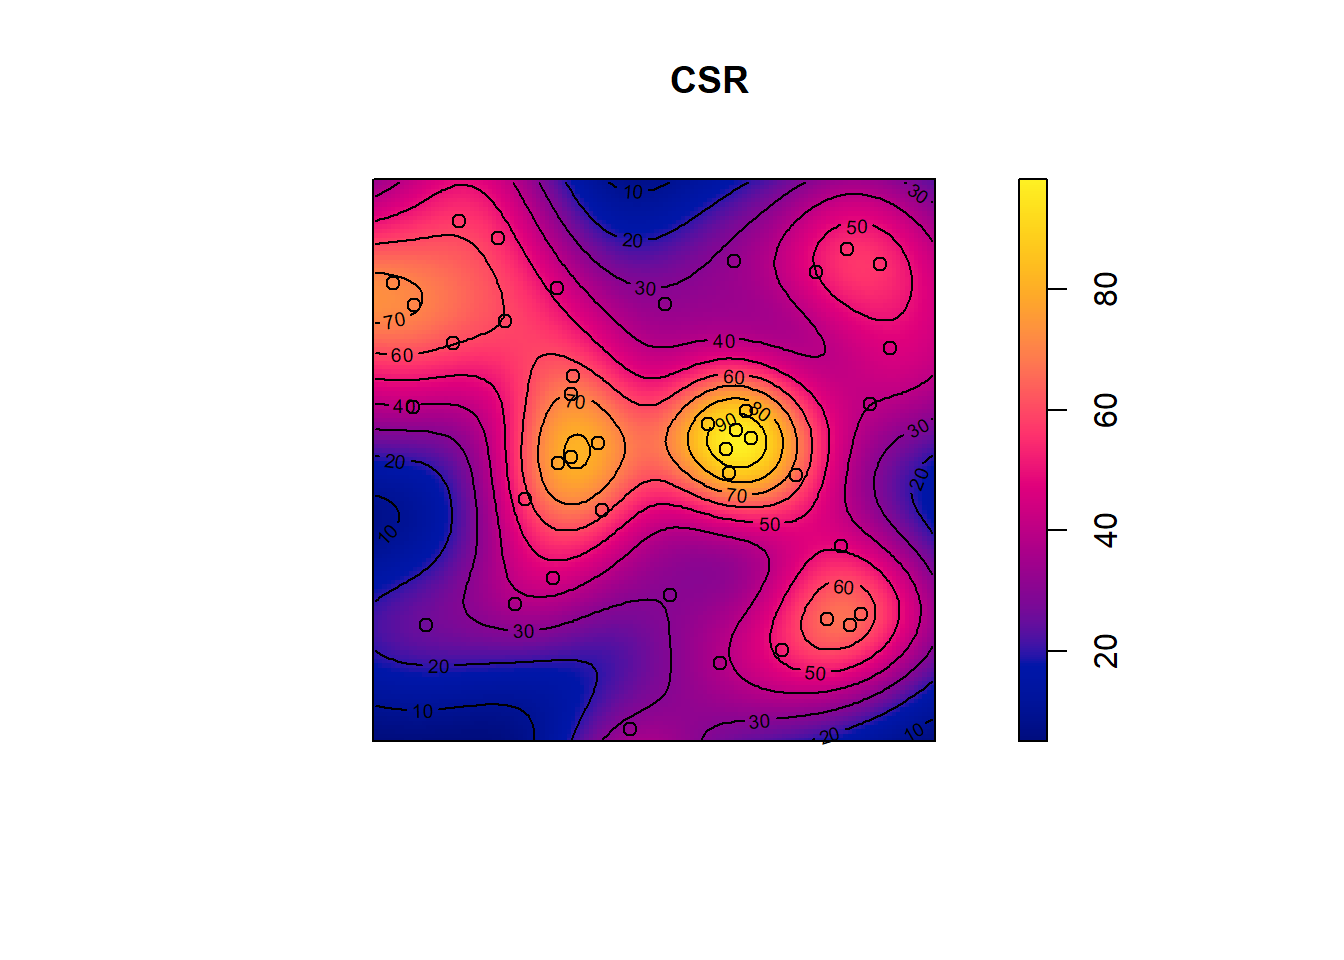
\includegraphics{Applied-Spatial-Data-Analysis_files/figure-latex/unnamed-chunk-23-1.pdf}

\hypertarget{regular-pattern}{%
\subsection{Regular Pattern}\label{regular-pattern}}

\begin{Shaded}
\begin{Highlighting}[]
\NormalTok{den <-}\StringTok{ }\KeywordTok{density}\NormalTok{(pp_regular)}
\KeywordTok{plot}\NormalTok{(den, }\DataTypeTok{main =} \StringTok{"Regular"}\NormalTok{)}
\KeywordTok{plot}\NormalTok{(pp_regular, }\DataTypeTok{add=}\OtherTok{TRUE}\NormalTok{)}
\KeywordTok{contour}\NormalTok{(den, }\DataTypeTok{add=}\OtherTok{TRUE}\NormalTok{)}
\end{Highlighting}
\end{Shaded}

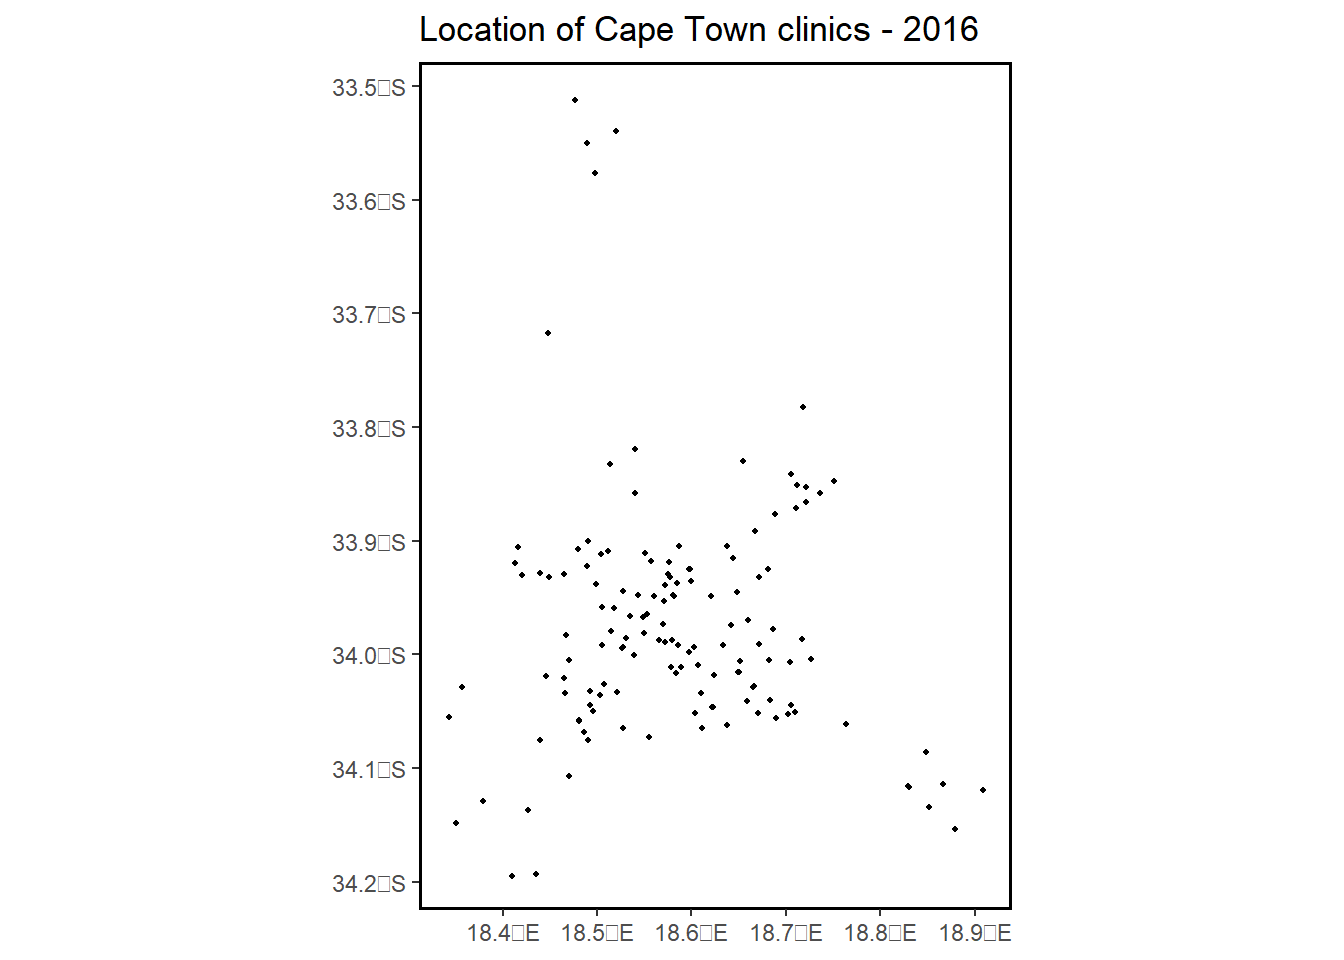
\includegraphics{Applied-Spatial-Data-Analysis_files/figure-latex/unnamed-chunk-24-1.pdf}

\hypertarget{cluster-pattern}{%
\subsection{Cluster Pattern}\label{cluster-pattern}}

\begin{Shaded}
\begin{Highlighting}[]
\NormalTok{den <-}\StringTok{ }\KeywordTok{density}\NormalTok{(pp_cluster)}
\KeywordTok{plot}\NormalTok{(den, }\DataTypeTok{main =} \StringTok{"Cluster"}\NormalTok{)}
\KeywordTok{plot}\NormalTok{(pp_cluster, }\DataTypeTok{add=}\OtherTok{TRUE}\NormalTok{)}
\KeywordTok{contour}\NormalTok{(den, }\DataTypeTok{add=}\OtherTok{TRUE}\NormalTok{)}
\end{Highlighting}
\end{Shaded}

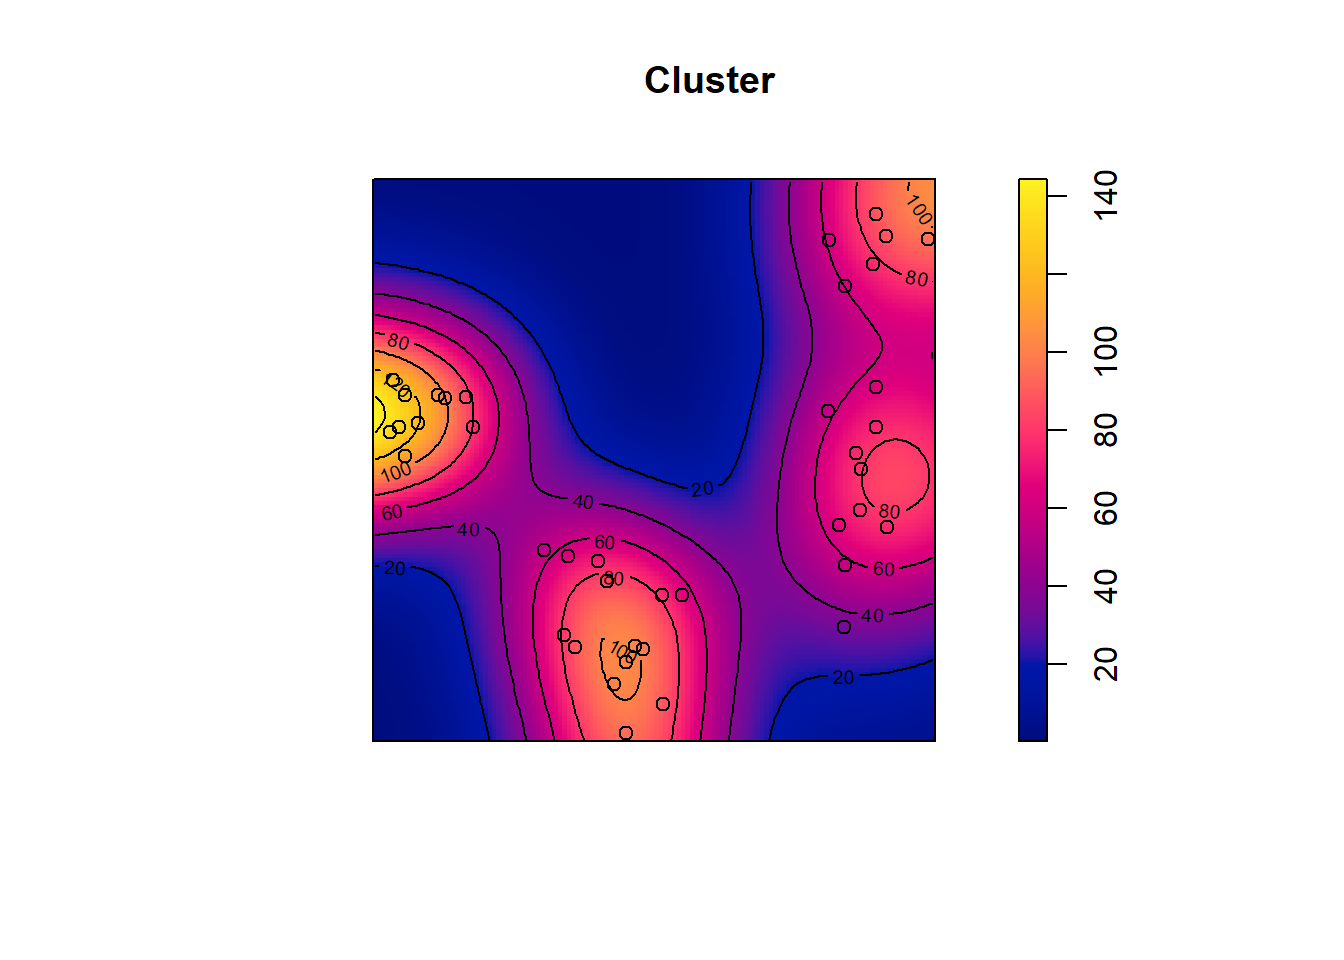
\includegraphics{Applied-Spatial-Data-Analysis_files/figure-latex/unnamed-chunk-25-1.pdf}

\hypertarget{kernel-smoothing-with-a-covariate}{%
\section{Kernel Smoothing with a Covariate}\label{kernel-smoothing-with-a-covariate}}

\hypertarget{tropical-rain-forest-trees-dataset}{%
\subsection{Tropical rain forest trees dataset}\label{tropical-rain-forest-trees-dataset}}

\begin{Shaded}
\begin{Highlighting}[]
\KeywordTok{data}\NormalTok{(}\StringTok{"bei"}\NormalTok{)}
\end{Highlighting}
\end{Shaded}

Assign the elevation covariate to a variable elev by typing

\begin{Shaded}
\begin{Highlighting}[]
\NormalTok{elev <-}\StringTok{ }\NormalTok{bei.extra}\OperatorTok{$}\NormalTok{elev}
\end{Highlighting}
\end{Shaded}

Plot the trees on top of an image of the elevation covariate.

\begin{Shaded}
\begin{Highlighting}[]
\KeywordTok{plot}\NormalTok{(elev, }\DataTypeTok{main =} \StringTok{""}\NormalTok{)}
\KeywordTok{plot}\NormalTok{(bei, }\DataTypeTok{add =} \OtherTok{TRUE}\NormalTok{, }\DataTypeTok{cex =} \FloatTok{0.3}\NormalTok{, }\DataTypeTok{pch =} \DecValTok{16}\NormalTok{, }\DataTypeTok{cols =} \StringTok{"white"}\NormalTok{)}
\end{Highlighting}
\end{Shaded}

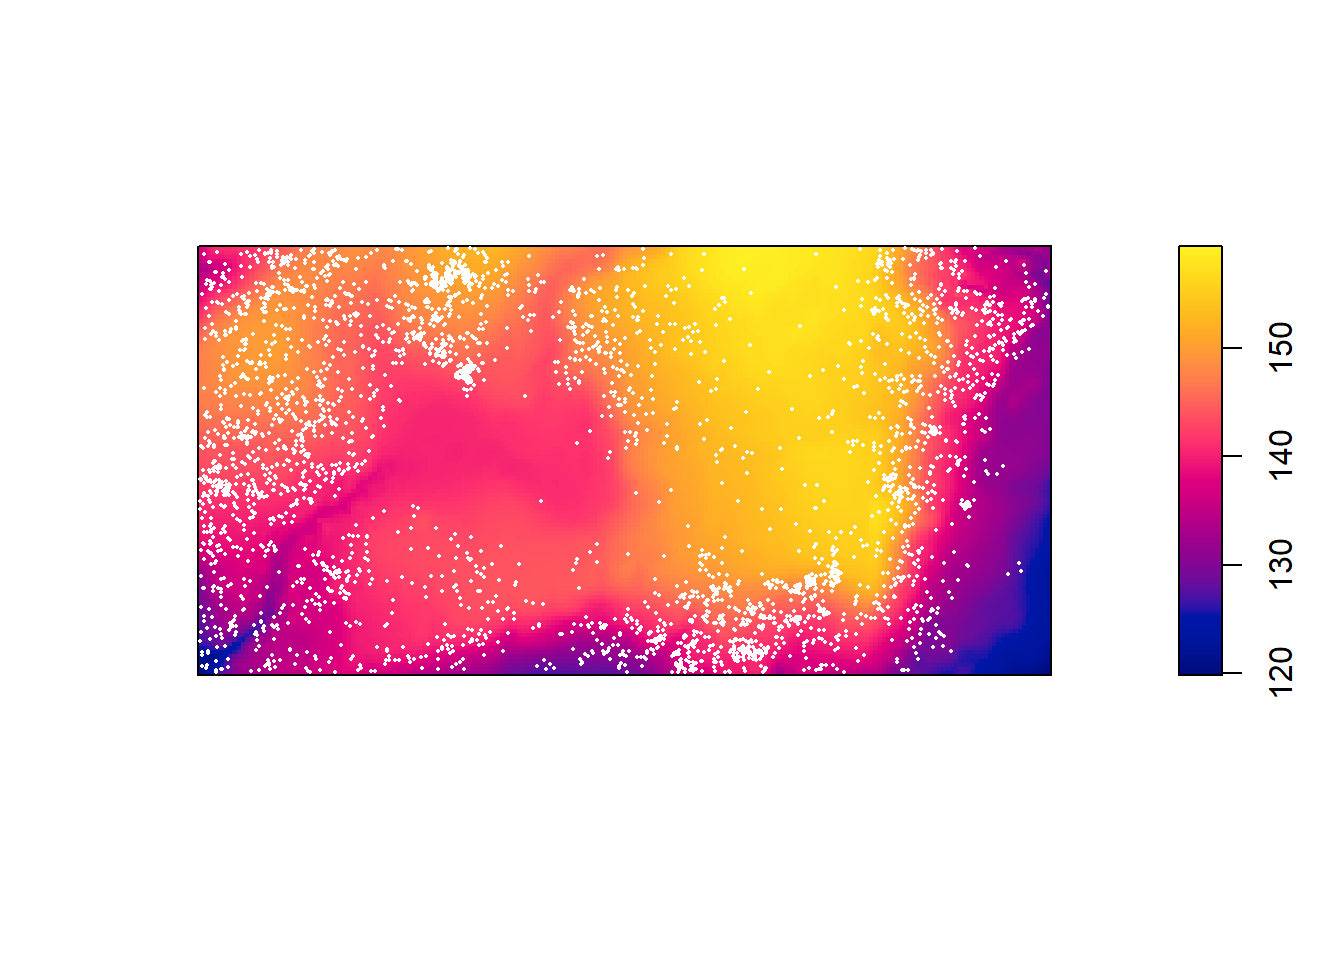
\includegraphics{Applied-Spatial-Data-Analysis_files/figure-latex/unnamed-chunk-28-1.pdf}

For the tropical rainforest data bei, it might be useful to split the study region into several
sub-regions according to the terrain elevation:

\begin{Shaded}
\begin{Highlighting}[]
\NormalTok{b <-}\StringTok{ }\KeywordTok{quantile}\NormalTok{(elev, }\DataTypeTok{probs=}\NormalTok{(}\DecValTok{0}\OperatorTok{:}\DecValTok{4}\NormalTok{)}\OperatorTok{/}\DecValTok{4}\NormalTok{, }\DataTypeTok{type=}\DecValTok{2}\NormalTok{)}

\NormalTok{Zcut <-}\StringTok{ }\KeywordTok{cut}\NormalTok{(elev, }\DataTypeTok{breaks=}\NormalTok{b, }\DataTypeTok{labels=}\KeywordTok{c}\NormalTok{(}\StringTok{"Low"}\NormalTok{, }\StringTok{"Med-Low"}\NormalTok{, }\StringTok{"Med-High"}\NormalTok{, }\StringTok{"High"}\NormalTok{))}
\KeywordTok{textureplot}\NormalTok{(Zcut, }\DataTypeTok{main =} \StringTok{""}\NormalTok{)}
\end{Highlighting}
\end{Shaded}

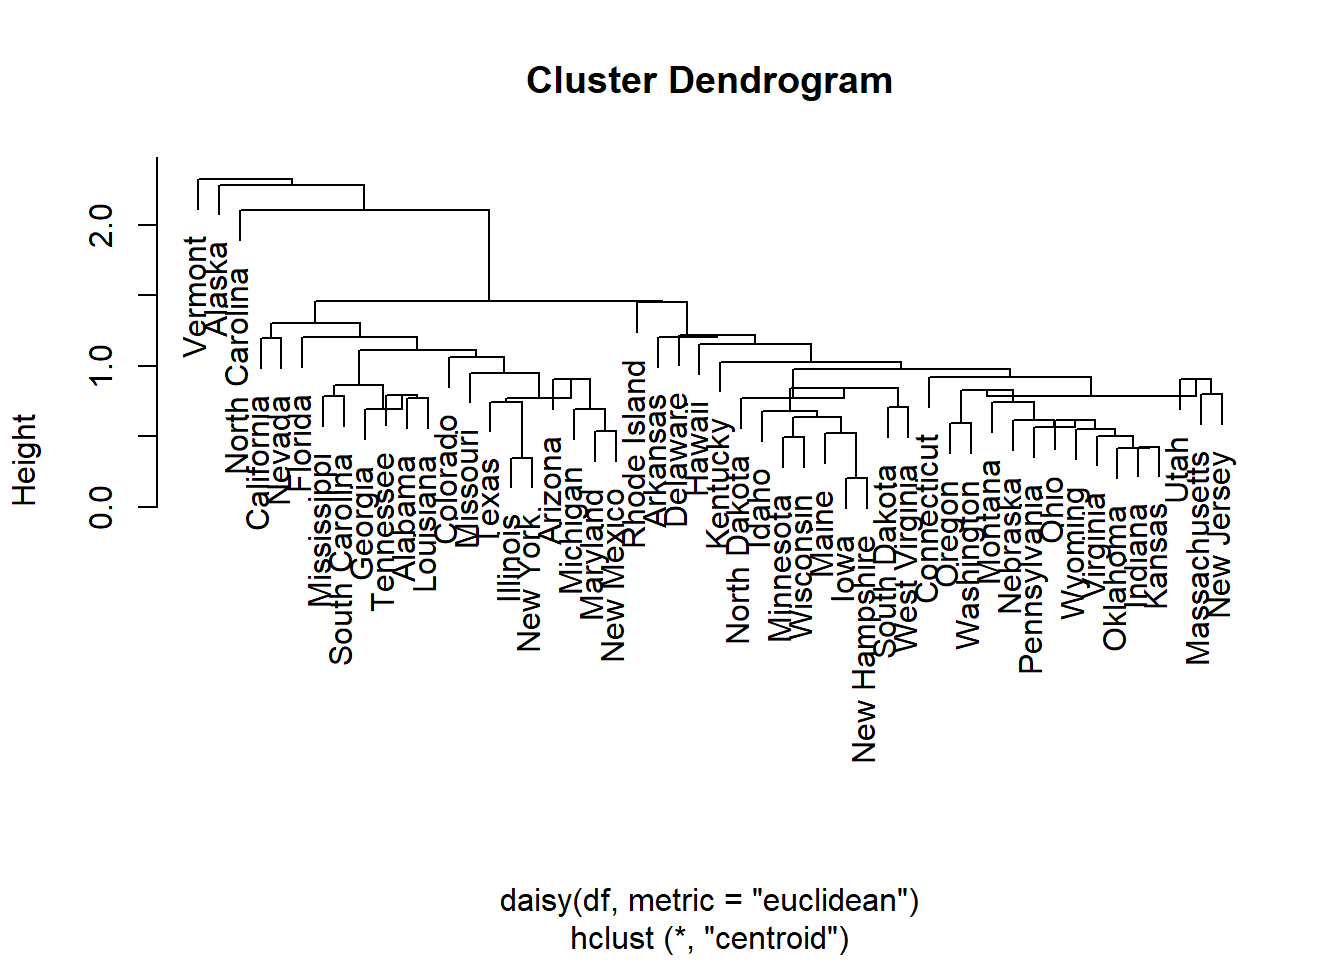
\includegraphics{Applied-Spatial-Data-Analysis_files/figure-latex/unnamed-chunk-29-1.pdf}

Convert the image from above to a tesselation, count the number of points in each region using quadratcount, and plot the quadrat counts.

\begin{Shaded}
\begin{Highlighting}[]
\NormalTok{V <-}\StringTok{ }\KeywordTok{tess}\NormalTok{(}\DataTypeTok{image=}\NormalTok{Zcut)}
\NormalTok{qc <-}\StringTok{ }\KeywordTok{quadratcount}\NormalTok{(bei, }\DataTypeTok{tess =}\NormalTok{ V)}
\NormalTok{qc}
\end{Highlighting}
\end{Shaded}

\begin{verbatim}
## tile
##      Low  Med-Low Med-High     High 
##      714      883     1344      663
\end{verbatim}

The output shows the number of trees in each region. Since the four regions have equal area, the counts should be approximately equal if there is a uniform density of trees. Obviously they are not equal; there appears to be a strong preference for higher elevations (dropping off for the highest elevations).

Estimate the intensity in each of the four regions.

\begin{Shaded}
\begin{Highlighting}[]
\KeywordTok{intensity}\NormalTok{(qc)}
\end{Highlighting}
\end{Shaded}

\begin{verbatim}
## tile
##         Low     Med-Low    Med-High        High 
## 0.005623154 0.006960978 0.010593103 0.005228707
\end{verbatim}

Assume that the intensity of trees is a function (\lambda(u) = \rho(e(u))) where (e(u)) is the terrain elevation at location u.

Compute a nonparametric estimate of the function (\rho) and plot it by

\begin{Shaded}
\begin{Highlighting}[]
\NormalTok{rh <-}\StringTok{ }\KeywordTok{rhohat}\NormalTok{(bei, elev)}
\KeywordTok{plot}\NormalTok{(rh)}
\end{Highlighting}
\end{Shaded}

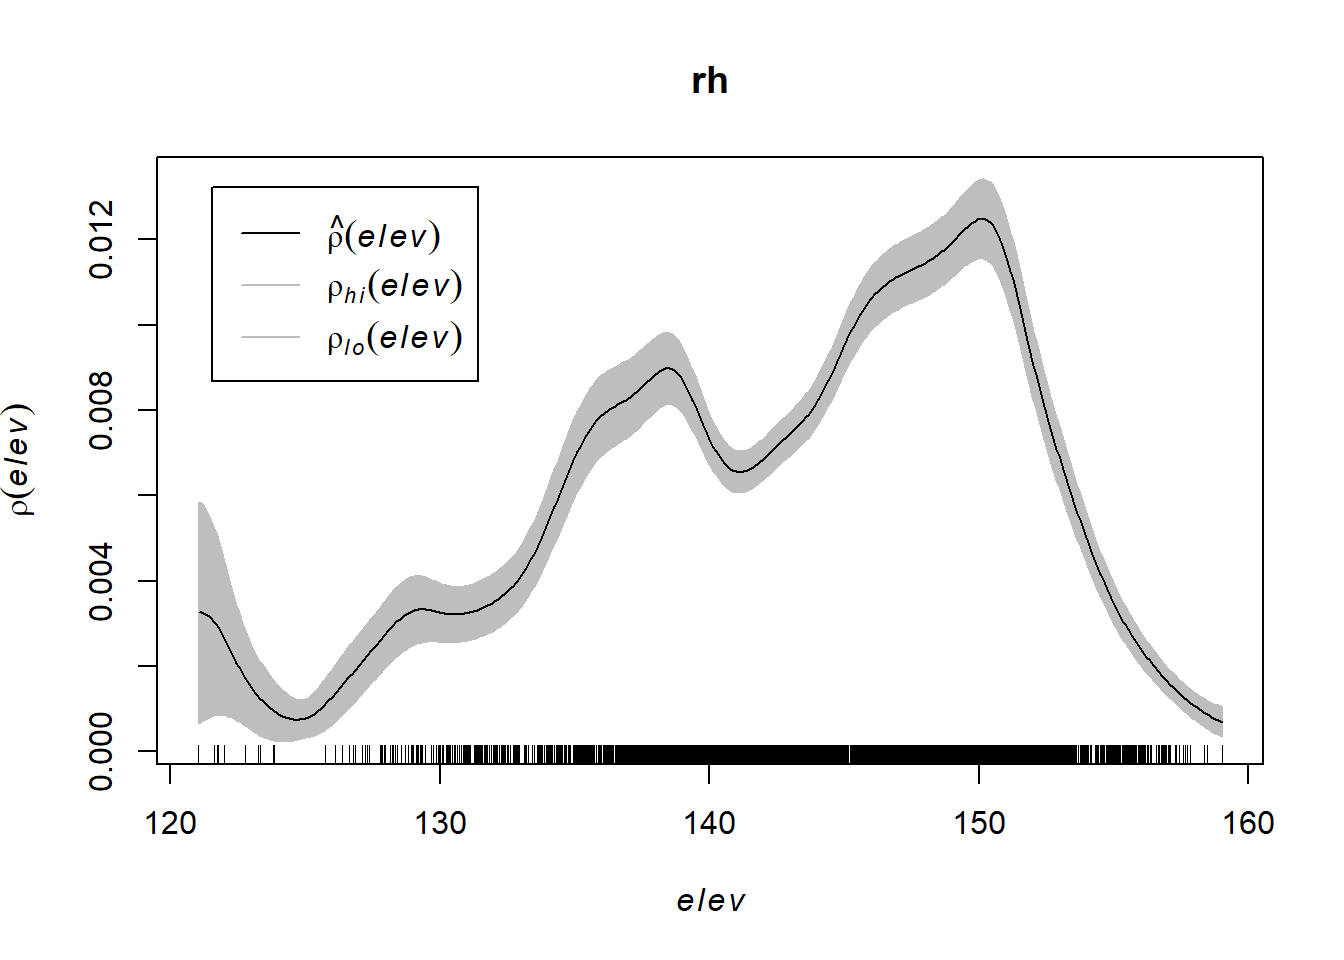
\includegraphics{Applied-Spatial-Data-Analysis_files/figure-latex/unnamed-chunk-32-1.pdf}

Compute the predicted intensity based on this estimate of (\rho).

\begin{Shaded}
\begin{Highlighting}[]
\NormalTok{predictedrho <-}\StringTok{ }\KeywordTok{predict}\NormalTok{(rh)}
\KeywordTok{plot}\NormalTok{(predictedrho, }\DataTypeTok{main =} \StringTok{""}\NormalTok{)}
\KeywordTok{plot}\NormalTok{(bei, }\DataTypeTok{add =} \OtherTok{TRUE}\NormalTok{, }\DataTypeTok{cols =} \StringTok{"white"}\NormalTok{, }\DataTypeTok{cex =} \FloatTok{.2}\NormalTok{, }\DataTypeTok{pch =} \DecValTok{16}\NormalTok{)}
\end{Highlighting}
\end{Shaded}

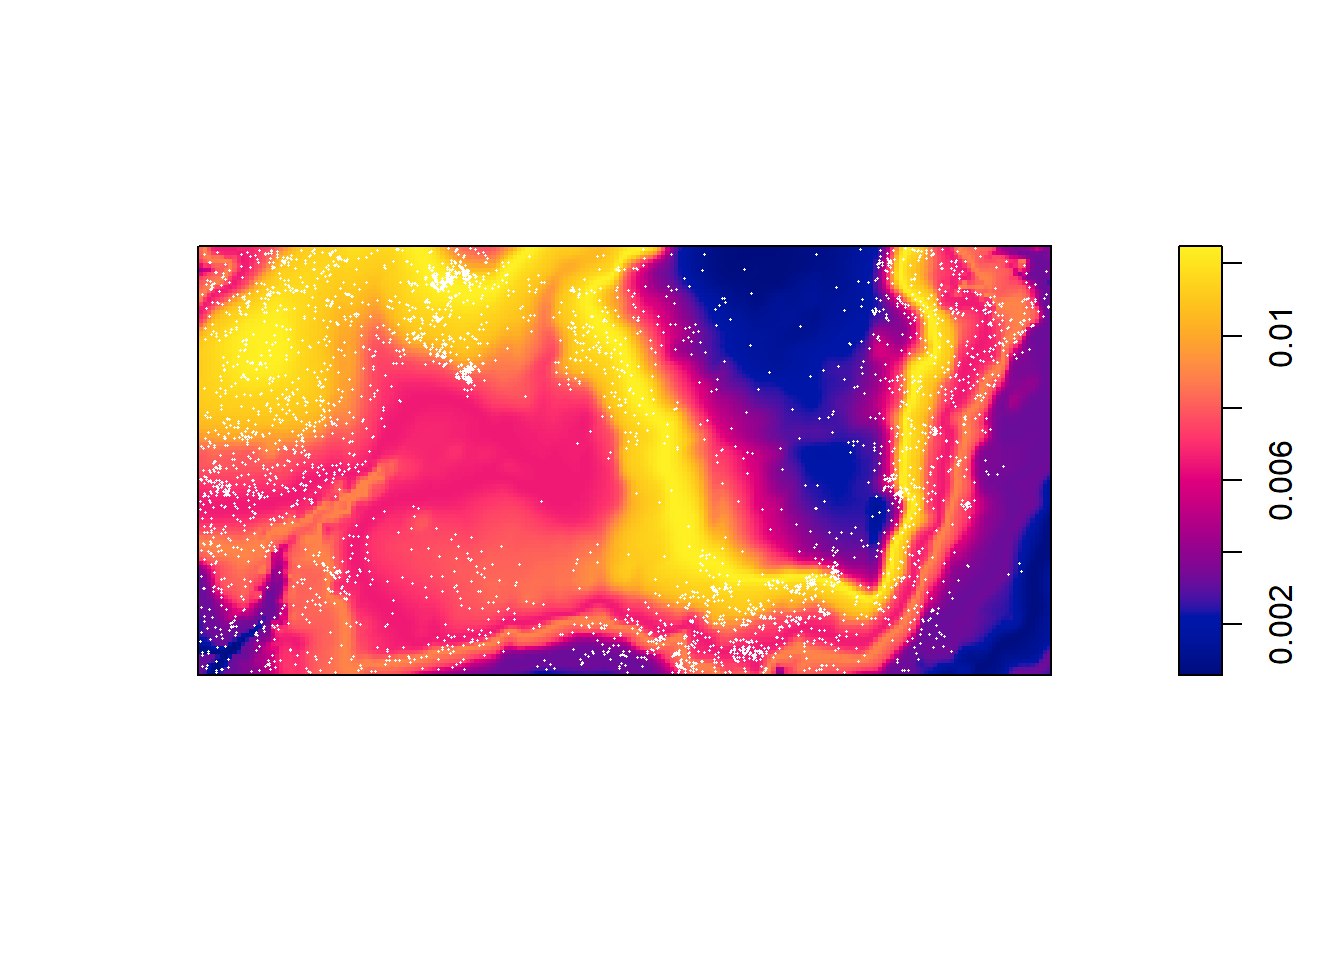
\includegraphics{Applied-Spatial-Data-Analysis_files/figure-latex/unnamed-chunk-33-1.pdf}

Compute a non-parametric estimate by kernel smoothing and compare with the predicted intensity above.

The kernel density estimate of the points is computed and plotted with the following code:

\begin{Shaded}
\begin{Highlighting}[]
\NormalTok{kerneldensity <-}\StringTok{ }\KeywordTok{density}\NormalTok{(bei, }\DataTypeTok{sigma =}\NormalTok{ bw.scott)}
\KeywordTok{plot}\NormalTok{(kerneldensity, }\DataTypeTok{main =} \StringTok{""}\NormalTok{)}
\KeywordTok{plot}\NormalTok{(kerneldensity, }\DataTypeTok{add =} \OtherTok{TRUE}\NormalTok{, }\DataTypeTok{cols =} \StringTok{"white"}\NormalTok{, }\DataTypeTok{cex =} \FloatTok{.2}\NormalTok{, }\DataTypeTok{pch =} \DecValTok{16}\NormalTok{)}
\end{Highlighting}
\end{Shaded}

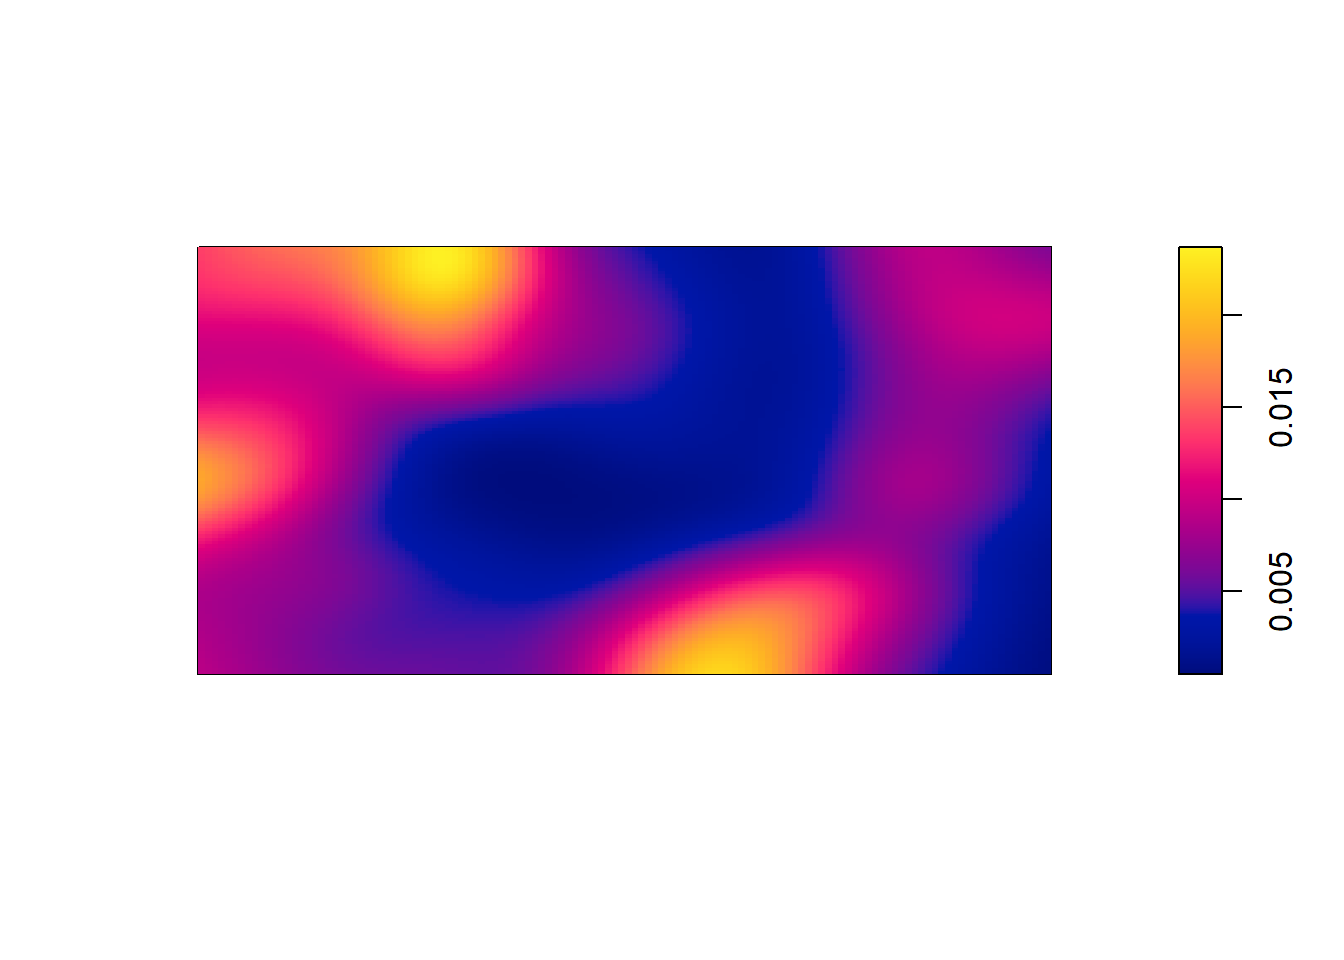
\includegraphics{Applied-Spatial-Data-Analysis_files/figure-latex/unnamed-chunk-34-1.pdf}

Compare the two

\begin{Shaded}
\begin{Highlighting}[]
\KeywordTok{pairs}\NormalTok{(predictedrho, kerneldensity)}
\end{Highlighting}
\end{Shaded}

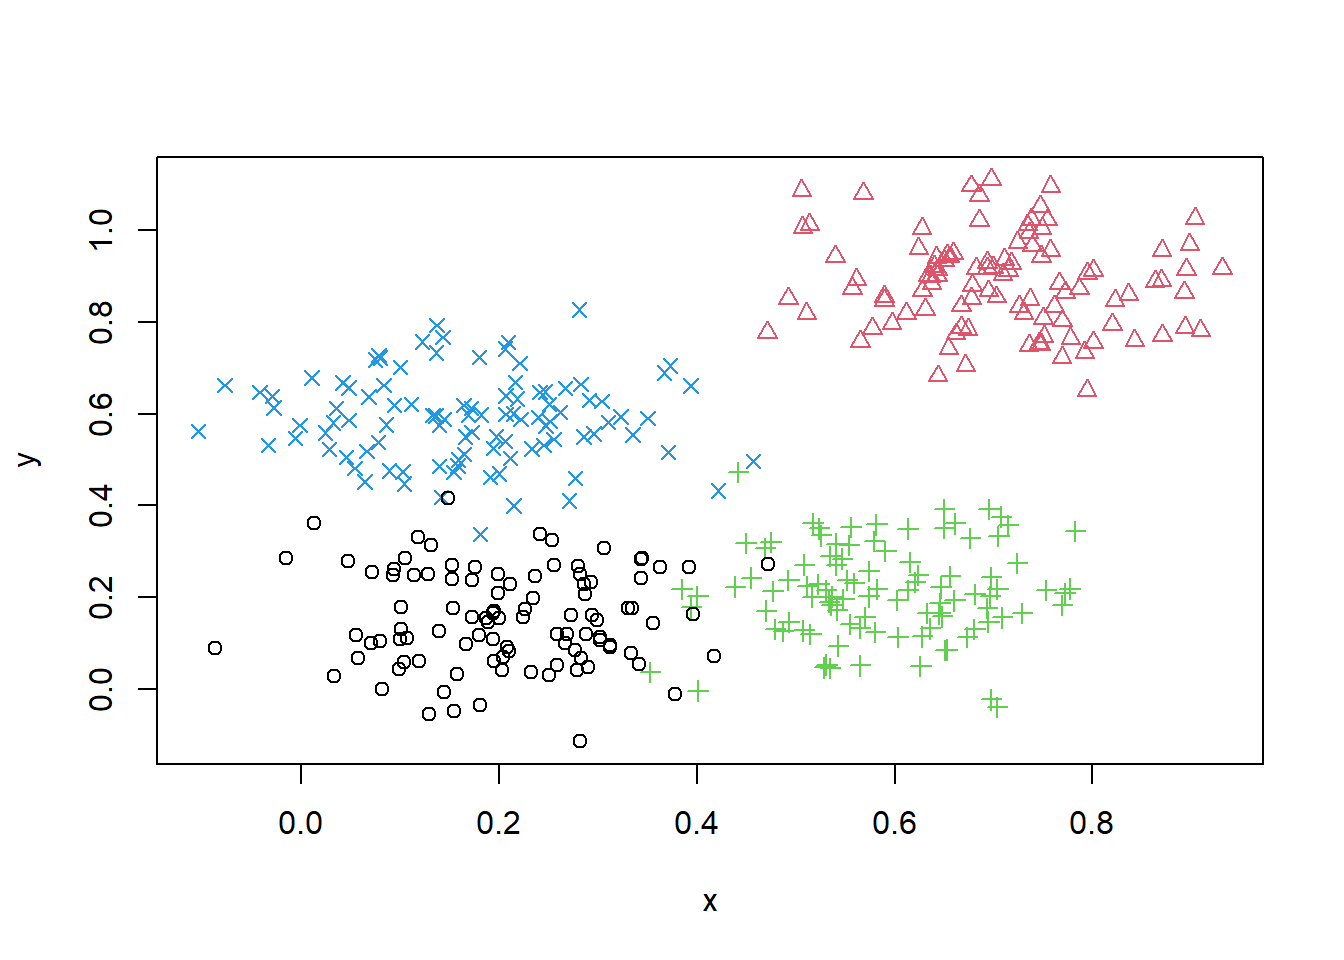
\includegraphics{Applied-Spatial-Data-Analysis_files/figure-latex/unnamed-chunk-35-1.pdf}

\begin{Shaded}
\begin{Highlighting}[]
\KeywordTok{plot}\NormalTok{(}\KeywordTok{eval.im}\NormalTok{(kerneldensity}\OperatorTok{-}\NormalTok{predictedrho))}
\end{Highlighting}
\end{Shaded}

\begin{verbatim}
## Warning: the images 'kerneldensity' and 'predictedrho' were not compatible
\end{verbatim}

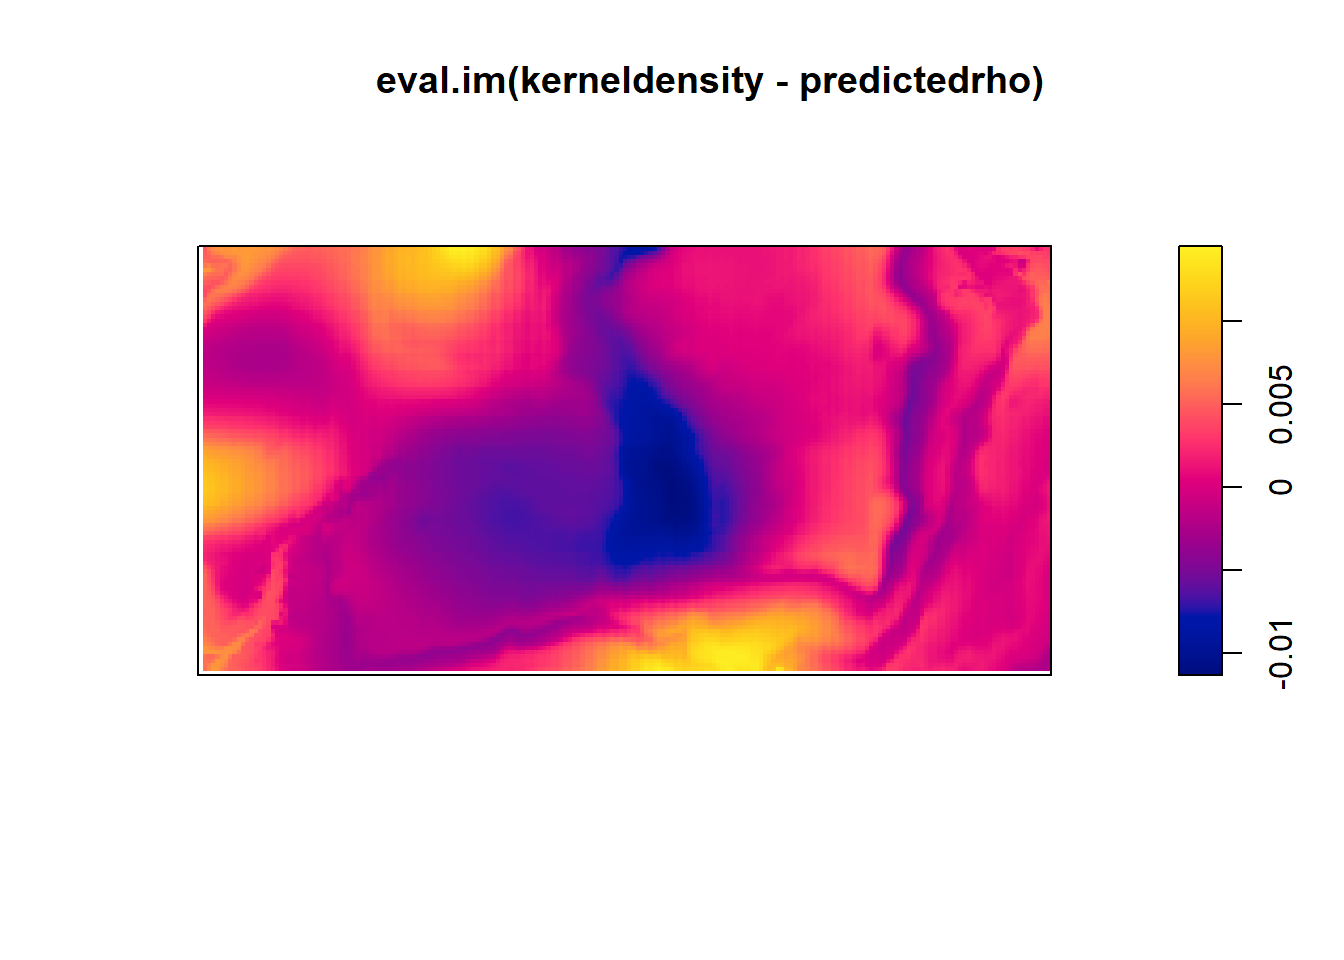
\includegraphics{Applied-Spatial-Data-Analysis_files/figure-latex/unnamed-chunk-35-2.pdf}

Which seems to be quite different form the predicted intensity.

\hypertarget{distance-measures-and-tests}{%
\section{Distance Measures and Tests}\label{distance-measures-and-tests}}

\hypertarget{e2e-distances}{%
\subsection{e2e Distances}\label{e2e-distances}}

\hypertarget{swp-dataset-1}{%
\subsubsection{swp dataset}\label{swp-dataset-1}}

\begin{Shaded}
\begin{Highlighting}[]
\NormalTok{PD =}\StringTok{ }\KeywordTok{pairdist}\NormalTok{(swp)}
\KeywordTok{class}\NormalTok{(PD)}
\end{Highlighting}
\end{Shaded}

\begin{verbatim}
## [1] "matrix" "array"
\end{verbatim}

\begin{Shaded}
\begin{Highlighting}[]
\NormalTok{dm <-}\StringTok{ }\KeywordTok{as.matrix}\NormalTok{(PD)}
\NormalTok{dm[}\DecValTok{1}\OperatorTok{:}\DecValTok{5}\NormalTok{, }\DecValTok{1}\OperatorTok{:}\DecValTok{5}\NormalTok{]}
\end{Highlighting}
\end{Shaded}

\begin{verbatim}
##          [,1]     [,2]     [,3]     [,4]     [,5]
## [1,] 0.000000 2.700000 3.701351 1.503330 5.433231
## [2,] 2.700000 0.000000 1.004988 1.204159 2.765863
## [3,] 3.701351 1.004988 0.000000 2.200000 1.772005
## [4,] 1.503330 1.204159 2.200000 0.000000 3.931921
## [5,] 5.433231 2.765863 1.772005 3.931921 0.000000
\end{verbatim}

\begin{Shaded}
\begin{Highlighting}[]
\KeywordTok{diag}\NormalTok{(dm) <-}\StringTok{ }\OtherTok{NA}
\CommentTok{#dm[1:5, 1:5]}
\NormalTok{wdmin <-}\StringTok{ }\KeywordTok{apply}\NormalTok{(dm, }\DecValTok{1}\NormalTok{, which.min)}

\NormalTok{dmin <-}\StringTok{ }\KeywordTok{apply}\NormalTok{(dm, }\DecValTok{1}\NormalTok{, min, }\DataTypeTok{na.rm=}\OtherTok{TRUE}\NormalTok{)}
\KeywordTok{head}\NormalTok{(dmin)}
\end{Highlighting}
\end{Shaded}

\begin{verbatim}
## [1] 1.5033296 0.8544004 1.0049876 0.9055385 1.0770330 0.8544004
\end{verbatim}

\begin{Shaded}
\begin{Highlighting}[]
\CommentTok{# which is the same as nndist e2e=nndist(swp)}

\NormalTok{dmin =}\StringTok{ }\KeywordTok{nndist}\NormalTok{(swp)}

\KeywordTok{plot}\NormalTok{(swp)}
\NormalTok{xy =}\StringTok{ }\KeywordTok{cbind}\NormalTok{(swp}\OperatorTok{$}\NormalTok{x, swp}\OperatorTok{$}\NormalTok{y)}

\NormalTok{ord <-}\StringTok{ }\KeywordTok{rev}\NormalTok{(}\KeywordTok{order}\NormalTok{(dmin))}
\NormalTok{far25 <-}\StringTok{ }\NormalTok{ord[}\DecValTok{1}\OperatorTok{:}\DecValTok{71}\NormalTok{]}
\NormalTok{neighbors <-}\StringTok{ }\NormalTok{wdmin[far25]}
\KeywordTok{points}\NormalTok{(xy[far25, ], }\DataTypeTok{col=}\StringTok{'blue'}\NormalTok{, }\DataTypeTok{pch=}\DecValTok{20}\NormalTok{)}
\KeywordTok{points}\NormalTok{(xy[neighbors, ], }\DataTypeTok{col=}\StringTok{'red'}\NormalTok{)}
\CommentTok{# drawing the lines, easiest via a loop}
\ControlFlowTok{for}\NormalTok{ (i }\ControlFlowTok{in}\NormalTok{ far25) \{}
    \KeywordTok{lines}\NormalTok{(}\KeywordTok{rbind}\NormalTok{(xy[i, ], xy[wdmin[i], ]), }\DataTypeTok{col=}\StringTok{'red'}\NormalTok{)}
\NormalTok{\}}
\end{Highlighting}
\end{Shaded}

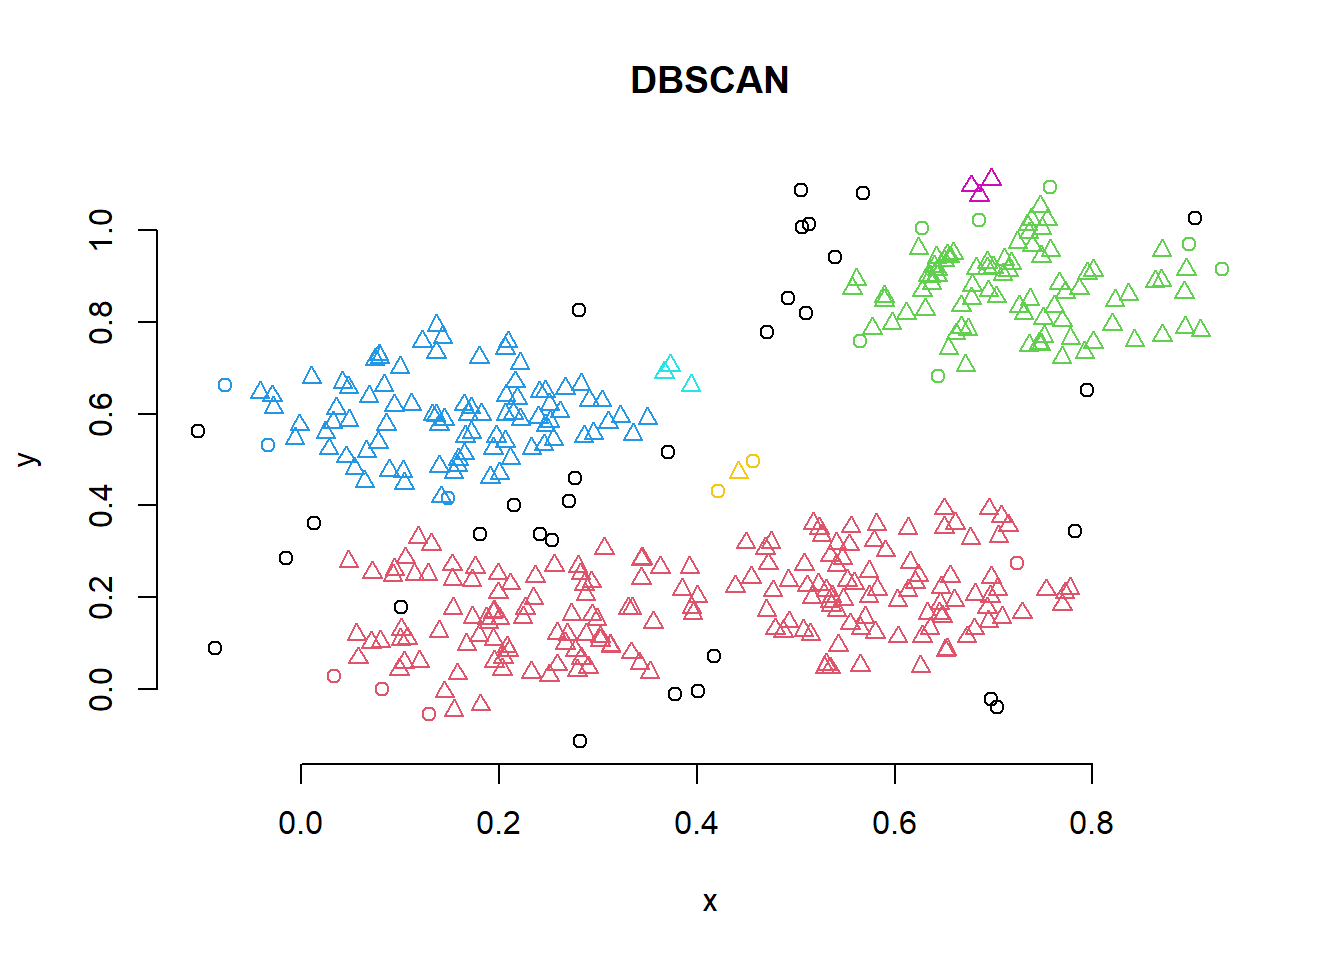
\includegraphics{Applied-Spatial-Data-Analysis_files/figure-latex/unnamed-chunk-36-1.pdf}

\hypertarget{simulated-csr-pattern-1}{%
\subsubsection{Simulated CSR Pattern}\label{simulated-csr-pattern-1}}

\begin{Shaded}
\begin{Highlighting}[]
\NormalTok{e2e_csr =}\StringTok{ }\KeywordTok{nndist}\NormalTok{(pp_csr)}
\NormalTok{e2e_csr}
\end{Highlighting}
\end{Shaded}

\begin{verbatim}
##  [1] 0.11056220 0.05419105 0.08163249 0.05574520 0.19907565 0.03191166
##  [7] 0.10456756 0.15049858 0.16325765 0.02841510 0.05044346 0.05419105
## [13] 0.10456756 0.07525211 0.02471890 0.08651227 0.03700818 0.06471165
## [19] 0.12663659 0.08163249 0.06471165 0.07525211 0.14362670 0.03195288
## [25] 0.09669706 0.03195288 0.09731910 0.04284774 0.11297958 0.03191166
## [31] 0.13454666 0.02841510 0.02471890 0.06711512 0.10924574 0.04269836
## [37] 0.09947882 0.03815278 0.14362670 0.10235020
\end{verbatim}

\begin{Shaded}
\begin{Highlighting}[]
\NormalTok{PD =}\StringTok{ }\KeywordTok{pairdist}\NormalTok{(pp_csr)}
\KeywordTok{class}\NormalTok{(PD)}
\end{Highlighting}
\end{Shaded}

\begin{verbatim}
## [1] "matrix" "array"
\end{verbatim}

\begin{Shaded}
\begin{Highlighting}[]
\NormalTok{dm <-}\StringTok{ }\KeywordTok{as.matrix}\NormalTok{(PD)}
\NormalTok{dm[}\DecValTok{1}\OperatorTok{:}\DecValTok{5}\NormalTok{, }\DecValTok{1}\OperatorTok{:}\DecValTok{5}\NormalTok{]}
\end{Highlighting}
\end{Shaded}

\begin{verbatim}
##           [,1]      [,2]      [,3]      [,4]      [,5]
## [1,] 0.0000000 0.2930205 0.5163115 0.2844957 0.7955061
## [2,] 0.2930205 0.0000000 0.5975953 0.4633681 0.8993362
## [3,] 0.5163115 0.5975953 0.0000000 0.2546708 0.3017974
## [4,] 0.2844957 0.4633681 0.2546708 0.0000000 0.5130861
## [5,] 0.7955061 0.8993362 0.3017974 0.5130861 0.0000000
\end{verbatim}

\begin{Shaded}
\begin{Highlighting}[]
\KeywordTok{diag}\NormalTok{(dm) <-}\StringTok{ }\OtherTok{NA}
\CommentTok{#dm[1:5, 1:5]}
\NormalTok{wdmin <-}\StringTok{ }\KeywordTok{apply}\NormalTok{(dm, }\DecValTok{1}\NormalTok{, which.min)}

\NormalTok{dmin <-}\StringTok{ }\KeywordTok{apply}\NormalTok{(dm, }\DecValTok{1}\NormalTok{, min, }\DataTypeTok{na.rm=}\OtherTok{TRUE}\NormalTok{)}
\KeywordTok{head}\NormalTok{(dmin)}
\end{Highlighting}
\end{Shaded}

\begin{verbatim}
## [1] 0.11056220 0.05419105 0.08163249 0.05574520 0.19907565 0.03191166
\end{verbatim}

\begin{Shaded}
\begin{Highlighting}[]
\CommentTok{# which is the same as nndist e2e=nndist(swp)}

\NormalTok{dmin =}\StringTok{ }\KeywordTok{nndist}\NormalTok{(pp_csr)}

\KeywordTok{plot}\NormalTok{(pp_csr)}
\NormalTok{xy =}\StringTok{ }\KeywordTok{cbind}\NormalTok{(pp_csr}\OperatorTok{$}\NormalTok{x, pp_csr}\OperatorTok{$}\NormalTok{y)}

\NormalTok{ord <-}\StringTok{ }\KeywordTok{rev}\NormalTok{(}\KeywordTok{order}\NormalTok{(dmin))}
\NormalTok{far25 <-}\StringTok{ }\NormalTok{ord[}\DecValTok{1}\OperatorTok{:}\DecValTok{40}\NormalTok{]}
\NormalTok{neighbors <-}\StringTok{ }\NormalTok{wdmin[far25]}
\KeywordTok{points}\NormalTok{(xy[far25, ], }\DataTypeTok{col=}\StringTok{'blue'}\NormalTok{, }\DataTypeTok{pch=}\DecValTok{20}\NormalTok{)}
\KeywordTok{points}\NormalTok{(xy[neighbors, ], }\DataTypeTok{col=}\StringTok{'red'}\NormalTok{)}
\CommentTok{# drawing the lines, easiest via a loop}
\ControlFlowTok{for}\NormalTok{ (i }\ControlFlowTok{in}\NormalTok{ far25) \{}
    \KeywordTok{lines}\NormalTok{(}\KeywordTok{rbind}\NormalTok{(xy[i, ], xy[wdmin[i], ]), }\DataTypeTok{col=}\StringTok{'red'}\NormalTok{)}
\NormalTok{\}}
\end{Highlighting}
\end{Shaded}

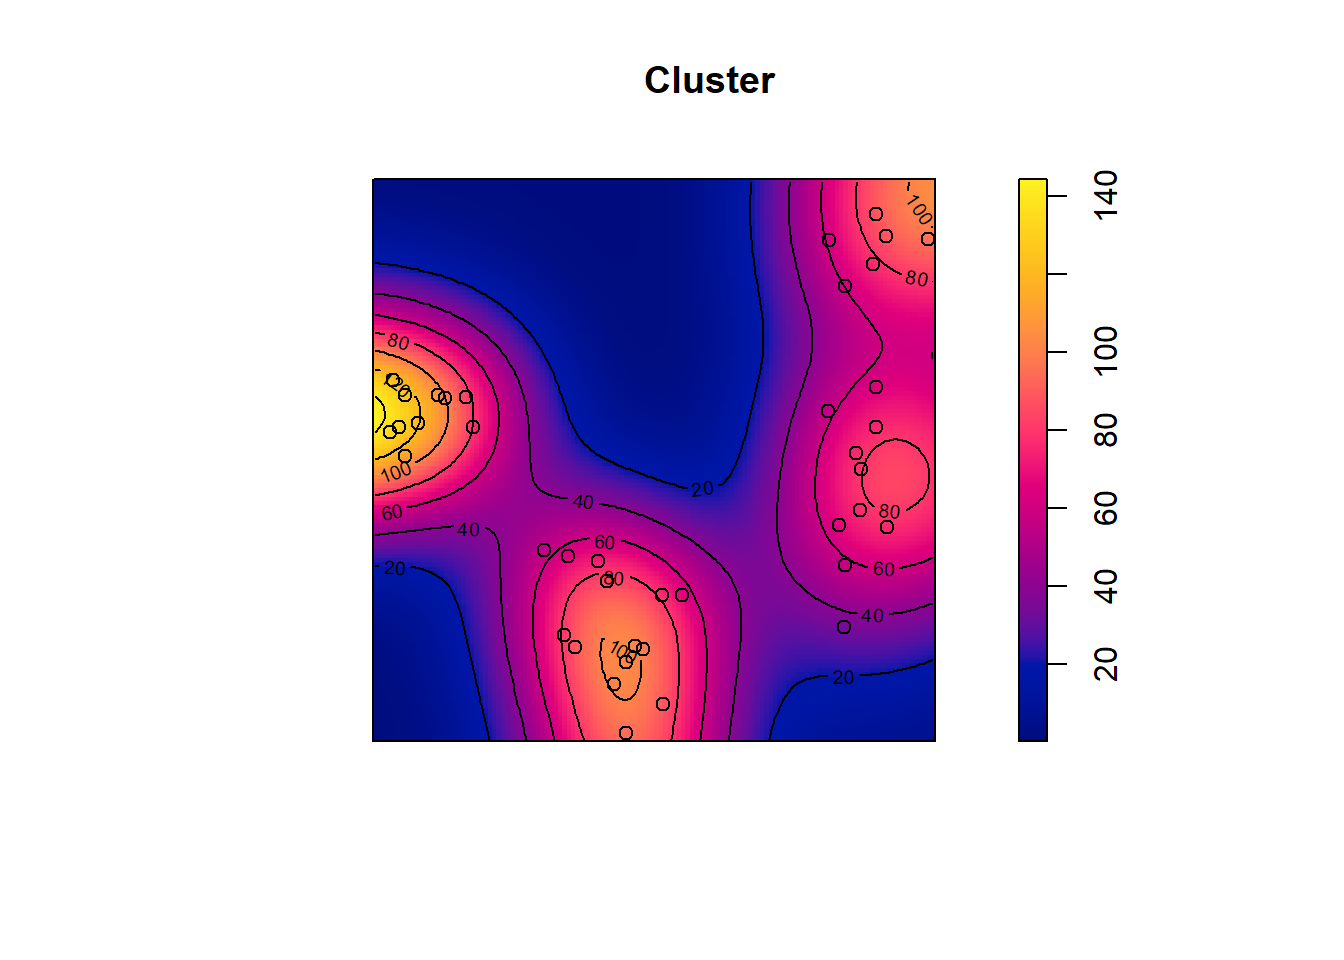
\includegraphics{Applied-Spatial-Data-Analysis_files/figure-latex/unnamed-chunk-38-1.pdf}

\hypertarget{simulated-cluster-pattern-1}{%
\subsubsection{Simulated Cluster Pattern}\label{simulated-cluster-pattern-1}}

\begin{Shaded}
\begin{Highlighting}[]
\NormalTok{e2e_cluster =}\StringTok{ }\KeywordTok{nndist}\NormalTok{(pp_cluster)}
\NormalTok{e2e_cluster}
\end{Highlighting}
\end{Shaded}

\begin{verbatim}
##  [1] 0.01854666 0.03502091 0.01854666 0.04969353 0.03502091 0.03390187
##  [7] 0.01268286 0.05624330 0.01268286 0.03830134 0.04275255 0.02983313
## [13] 0.04275255 0.02983313 0.03774271 0.03774271 0.03391843 0.01376367
## [19] 0.01376367 0.03500058 0.08344093 0.06403124 0.05422191 0.08344093
## [25] 0.03500058 0.08988091 0.04304986 0.07202173 0.04586212 0.02906394
## [31] 0.08760076 0.11053898 0.04586212 0.02906394 0.05896243 0.07149045
## [37] 0.04361429 0.04361429 0.05745563 0.07483198
\end{verbatim}

\begin{Shaded}
\begin{Highlighting}[]
\NormalTok{PD_cluster =}\StringTok{ }\KeywordTok{pairdist}\NormalTok{(pp_cluster)}
\KeywordTok{class}\NormalTok{(PD_cluster)}
\end{Highlighting}
\end{Shaded}

\begin{verbatim}
## [1] "matrix" "array"
\end{verbatim}

\begin{Shaded}
\begin{Highlighting}[]
\NormalTok{dm_cluster <-}\StringTok{ }\KeywordTok{as.matrix}\NormalTok{(PD_cluster)}
\NormalTok{dm_cluster[}\DecValTok{1}\OperatorTok{:}\DecValTok{5}\NormalTok{, }\DecValTok{1}\OperatorTok{:}\DecValTok{5}\NormalTok{]}
\end{Highlighting}
\end{Shaded}

\begin{verbatim}
##            [,1]       [,2]       [,3]       [,4]       [,5]
## [1,] 0.00000000 0.09345138 0.01854666 0.04969353 0.07093497
## [2,] 0.09345138 0.00000000 0.08597921 0.13688899 0.03502091
## [3,] 0.01854666 0.08597921 0.00000000 0.05097721 0.05847323
## [4,] 0.04969353 0.13688899 0.05097721 0.00000000 0.10757315
## [5,] 0.07093497 0.03502091 0.05847323 0.10757315 0.00000000
\end{verbatim}

\begin{Shaded}
\begin{Highlighting}[]
\KeywordTok{diag}\NormalTok{(dm_cluster) <-}\StringTok{ }\OtherTok{NA}
\NormalTok{wdmin_cluster <-}\StringTok{ }\KeywordTok{apply}\NormalTok{(dm_cluster, }\DecValTok{1}\NormalTok{, which.min)}

\NormalTok{dmin_cluster <-}\StringTok{ }\KeywordTok{apply}\NormalTok{(dm_cluster, }\DecValTok{1}\NormalTok{, min, }\DataTypeTok{na.rm=}\OtherTok{TRUE}\NormalTok{)}
\KeywordTok{head}\NormalTok{(dmin}\OperatorTok{-}\NormalTok{cluster)}
\end{Highlighting}
\end{Shaded}

\begin{verbatim}
##              X          Y
## 1  0.080388175 -0.4397788
## 2  0.018557146 -0.5894417
## 3  0.034750612 -0.4767600
## 4 -0.001070259 -0.4526473
## 5  0.141971489 -0.4168896
## 6 -0.048015500 -0.5340536
\end{verbatim}

\begin{Shaded}
\begin{Highlighting}[]
\CommentTok{# which is the same as nndist e2e=nndist(swp)}

\NormalTok{dmin_cluster =}\StringTok{ }\KeywordTok{nndist}\NormalTok{(pp_cluster)}

\KeywordTok{plot}\NormalTok{(pp_cluster)}
\NormalTok{xy_cluster =}\StringTok{ }\KeywordTok{cbind}\NormalTok{(pp_cluster}\OperatorTok{$}\NormalTok{x, pp_cluster}\OperatorTok{$}\NormalTok{y)}

\NormalTok{ord <-}\StringTok{ }\KeywordTok{rev}\NormalTok{(}\KeywordTok{order}\NormalTok{(dmin_cluster))}
\NormalTok{far25 <-}\StringTok{ }\NormalTok{ord[}\DecValTok{1}\OperatorTok{:}\DecValTok{40}\NormalTok{]}
\NormalTok{neighbors <-}\StringTok{ }\NormalTok{wdmin_cluster[far25]}
\KeywordTok{points}\NormalTok{(xy_cluster[far25, ], }\DataTypeTok{col=}\StringTok{'blue'}\NormalTok{, }\DataTypeTok{pch=}\DecValTok{20}\NormalTok{)}
\KeywordTok{points}\NormalTok{(xy_cluster[neighbors, ], }\DataTypeTok{col=}\StringTok{'red'}\NormalTok{)}
\CommentTok{# drawing the lines, easiest via a loop}
\ControlFlowTok{for}\NormalTok{ (i }\ControlFlowTok{in}\NormalTok{ far25) \{}
    \KeywordTok{lines}\NormalTok{(}\KeywordTok{rbind}\NormalTok{(xy_cluster[i, ], xy_cluster[wdmin_cluster[i], ]), }\DataTypeTok{col=}\StringTok{'red'}\NormalTok{)}
\NormalTok{\}}
\end{Highlighting}
\end{Shaded}

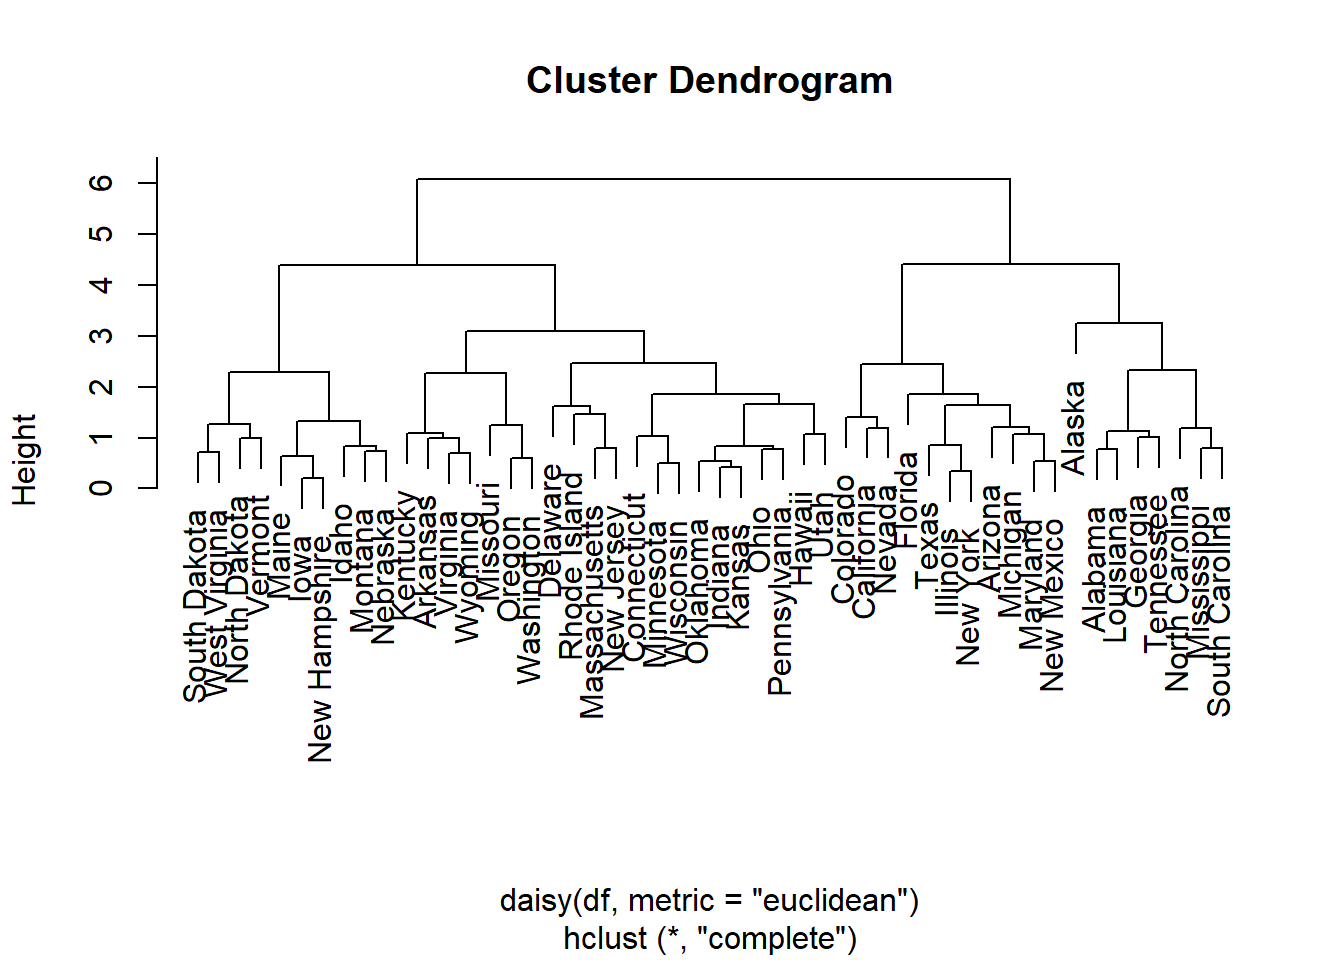
\includegraphics{Applied-Spatial-Data-Analysis_files/figure-latex/unnamed-chunk-40-1.pdf}

\hypertarget{simulated-regular-pattern-1}{%
\subsubsection{Simulated Regular Pattern}\label{simulated-regular-pattern-1}}

\begin{Shaded}
\begin{Highlighting}[]
\NormalTok{e2e_regular =}\StringTok{ }\KeywordTok{nndist}\NormalTok{(pp_regular)}
\NormalTok{e2e_regular}
\end{Highlighting}
\end{Shaded}

\begin{verbatim}
##  [1] 0.1111111 0.1111111 0.1111111 0.1111111 0.1111111 0.1111111 0.1111111
##  [8] 0.1111111 0.1111111 0.1111111 0.1111111 0.1111111 0.1111111 0.1111111
## [15] 0.1111111 0.1111111 0.1111111 0.1111111 0.1111111 0.1111111 0.1111111
## [22] 0.1111111 0.1111111 0.1111111 0.1111111 0.1111111 0.1111111 0.1111111
## [29] 0.1111111 0.1111111 0.1111111 0.1111111 0.1111111 0.1111111 0.1111111
## [36] 0.1111111 0.1111111 0.1111111 0.1111111 0.1111111
\end{verbatim}

\begin{Shaded}
\begin{Highlighting}[]
\NormalTok{PD_regular =}\StringTok{ }\KeywordTok{pairdist}\NormalTok{(pp_regular)}
\KeywordTok{class}\NormalTok{(PD_regular)}
\end{Highlighting}
\end{Shaded}

\begin{verbatim}
## [1] "matrix" "array"
\end{verbatim}

\begin{Shaded}
\begin{Highlighting}[]
\NormalTok{dm_regular <-}\StringTok{ }\KeywordTok{as.matrix}\NormalTok{(PD_regular)}
\NormalTok{dm_regular[}\DecValTok{1}\OperatorTok{:}\DecValTok{5}\NormalTok{, }\DecValTok{1}\OperatorTok{:}\DecValTok{5}\NormalTok{]}
\end{Highlighting}
\end{Shaded}

\begin{verbatim}
##           [,1]      [,2]      [,3]      [,4]      [,5]
## [1,] 0.0000000 0.1666667 0.3333333 0.5000000 0.6666667
## [2,] 0.1666667 0.0000000 0.1666667 0.3333333 0.5000000
## [3,] 0.3333333 0.1666667 0.0000000 0.1666667 0.3333333
## [4,] 0.5000000 0.3333333 0.1666667 0.0000000 0.1666667
## [5,] 0.6666667 0.5000000 0.3333333 0.1666667 0.0000000
\end{verbatim}

\begin{Shaded}
\begin{Highlighting}[]
\KeywordTok{diag}\NormalTok{(dm_regular) <-}\StringTok{ }\OtherTok{NA}
\NormalTok{wdmin_regular <-}\StringTok{ }\KeywordTok{apply}\NormalTok{(dm_regular, }\DecValTok{1}\NormalTok{, which.min)}

\NormalTok{dmin_regular <-}\StringTok{ }\KeywordTok{apply}\NormalTok{(dm_regular, }\DecValTok{1}\NormalTok{, min, }\DataTypeTok{na.rm=}\OtherTok{TRUE}\NormalTok{)}
\KeywordTok{head}\NormalTok{(dmin}\OperatorTok{-}\NormalTok{regular)}
\end{Highlighting}
\end{Shaded}

\begin{verbatim}
##             X             Y
## 1 -0.05610447 -0.0005489143
## 2 -0.27914228 -0.0569200607
## 3 -0.41836751 -0.0294786165
## 4 -0.61092147 -0.0553659112
## 5 -0.63425768  0.0879645408
## 6 -0.13475501 -0.1903105666
\end{verbatim}

\begin{Shaded}
\begin{Highlighting}[]
\CommentTok{# which is the same as nndist e2e=nndist(swp)}

\NormalTok{dmin_regular =}\StringTok{ }\KeywordTok{nndist}\NormalTok{(pp_regular)}

\KeywordTok{plot}\NormalTok{(pp_regular)}
\NormalTok{xy_regular =}\StringTok{ }\KeywordTok{cbind}\NormalTok{(pp_regular}\OperatorTok{$}\NormalTok{x, pp_regular}\OperatorTok{$}\NormalTok{y)}

\NormalTok{ord <-}\StringTok{ }\KeywordTok{rev}\NormalTok{(}\KeywordTok{order}\NormalTok{(dmin_regular))}
\NormalTok{far25 <-}\StringTok{ }\NormalTok{ord[}\DecValTok{1}\OperatorTok{:}\DecValTok{40}\NormalTok{]}
\NormalTok{neighbors <-}\StringTok{ }\NormalTok{wdmin_regular[far25]}
\KeywordTok{points}\NormalTok{(xy_regular[far25, ], }\DataTypeTok{col=}\StringTok{'blue'}\NormalTok{, }\DataTypeTok{pch=}\DecValTok{20}\NormalTok{)}
\KeywordTok{points}\NormalTok{(xy_regular[neighbors, ], }\DataTypeTok{col=}\StringTok{'red'}\NormalTok{)}
\CommentTok{# drawing the lines, easiest via a loop}
\ControlFlowTok{for}\NormalTok{ (i }\ControlFlowTok{in}\NormalTok{ far25) \{}
    \KeywordTok{lines}\NormalTok{(}\KeywordTok{rbind}\NormalTok{(xy_regular[i, ], xy_regular[wdmin_regular[i], ]), }\DataTypeTok{col=}\StringTok{'red'}\NormalTok{)}
\NormalTok{\}}
\end{Highlighting}
\end{Shaded}

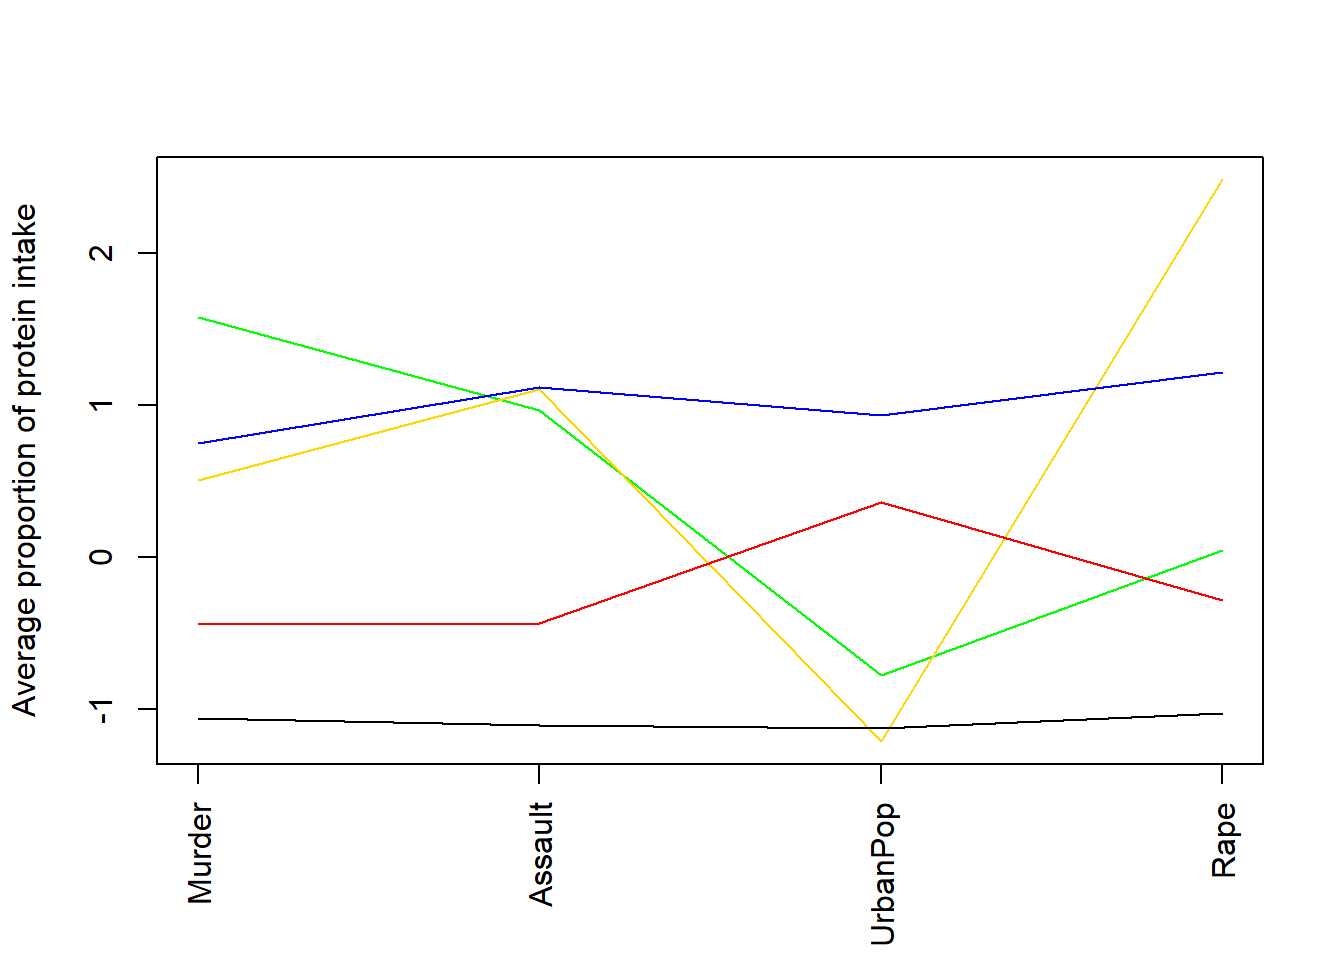
\includegraphics{Applied-Spatial-Data-Analysis_files/figure-latex/unnamed-chunk-42-1.pdf}

\hypertarget{p2e-distances}{%
\subsection{p2e Distances}\label{p2e-distances}}

Generate Random points

\begin{Shaded}
\begin{Highlighting}[]
\KeywordTok{set.seed}\NormalTok{(}\DecValTok{23}\NormalTok{)}
\NormalTok{randompoints =}\StringTok{ }\KeywordTok{matrix}\NormalTok{(}\KeywordTok{runif}\NormalTok{(}\DecValTok{60}\NormalTok{),}\DataTypeTok{ncol=}\DecValTok{2}\NormalTok{)}
\CommentTok{#randompoints = matrix(runif(250),ncol=2)}
\end{Highlighting}
\end{Shaded}

\hypertarget{csr-pattern-1}{%
\subsubsection{CSR Pattern}\label{csr-pattern-1}}

\begin{Shaded}
\begin{Highlighting}[]
\KeywordTok{plot}\NormalTok{(pp_csr)}
\KeywordTok{points}\NormalTok{(randompoints, }\DataTypeTok{col =} \StringTok{"blue"}\NormalTok{, }\DataTypeTok{pch=}\DecValTok{3}\NormalTok{)}
\end{Highlighting}
\end{Shaded}

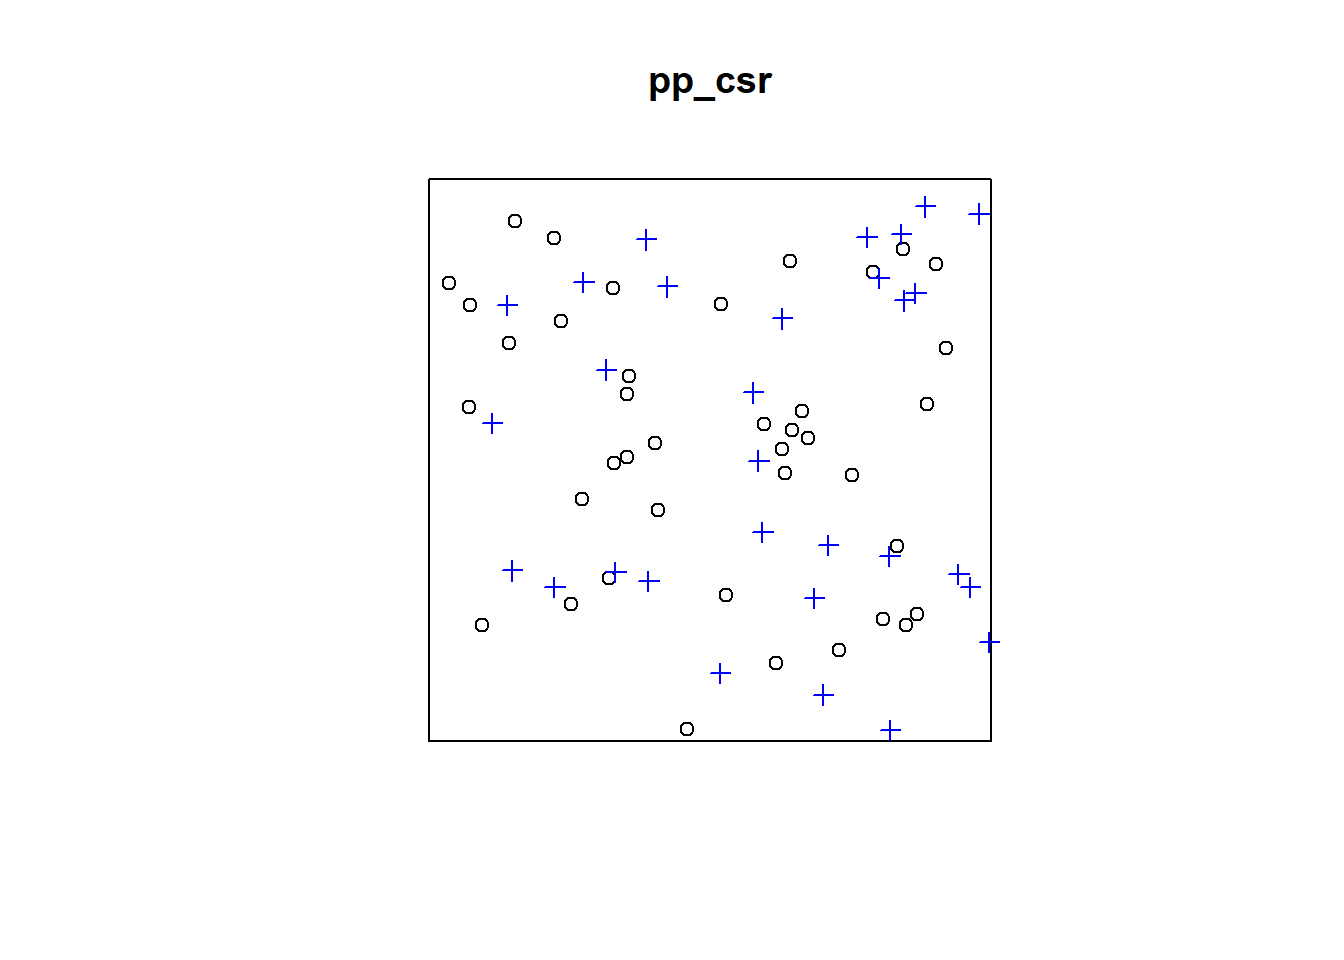
\includegraphics{Applied-Spatial-Data-Analysis_files/figure-latex/unnamed-chunk-44-1.pdf}

\begin{Shaded}
\begin{Highlighting}[]
\NormalTok{p2e_distances_csr =}\StringTok{ }\OtherTok{NULL}
\NormalTok{mins_csr =}\StringTok{ }\OtherTok{NULL}
\NormalTok{xy =}\StringTok{ }\KeywordTok{cbind}\NormalTok{(pp_csr}\OperatorTok{$}\NormalTok{x, pp_csr}\OperatorTok{$}\NormalTok{y)}


\CommentTok{# sqrt((xy[2,1]-randompoints[1,1])^2+(xy[2,2]-randompoints[1,2])^2)}
\CommentTok{# sqrt((xy[1,1]-randompoints[2,1])^2+(xy[1,2]-randompoints[2,2])^2)}


\ControlFlowTok{for}\NormalTok{(i }\ControlFlowTok{in} \DecValTok{1}\OperatorTok{:}\KeywordTok{dim}\NormalTok{(randompoints)[}\DecValTok{1}\NormalTok{])\{}
\NormalTok{dist1 =}\StringTok{ }\KeywordTok{matrix}\NormalTok{(}\KeywordTok{pairdist}\NormalTok{(}\KeywordTok{rbind}\NormalTok{(randompoints[i,],xy)),}\DecValTok{41}\NormalTok{)}

\NormalTok{p2e_distances_csr =}\StringTok{ }\KeywordTok{c}\NormalTok{(p2e_distances_csr,}\KeywordTok{min}\NormalTok{(dist1[}\DecValTok{2}\OperatorTok{:}\DecValTok{41}\NormalTok{,}\DecValTok{1}\NormalTok{]))}
\NormalTok{mins_csr =}\StringTok{ }\KeywordTok{c}\NormalTok{(mins_csr,}\KeywordTok{which.min}\NormalTok{(dist1[}\DecValTok{2}\OperatorTok{:}\DecValTok{41}\NormalTok{,}\DecValTok{1}\NormalTok{]))}
\NormalTok{\}}


\KeywordTok{plot}\NormalTok{(pp_csr)}
\NormalTok{ord <-}\StringTok{ }\KeywordTok{rev}\NormalTok{(}\KeywordTok{order}\NormalTok{(p2e_distances_csr))}
\NormalTok{far25 <-}\StringTok{ }\DecValTok{1}\OperatorTok{:}\KeywordTok{dim}\NormalTok{(randompoints)[}\DecValTok{1}\NormalTok{]}
\NormalTok{neighbors <-}\StringTok{ }\NormalTok{mins_csr}
\KeywordTok{points}\NormalTok{(randompoints, }\DataTypeTok{col=}\StringTok{'red'}\NormalTok{, }\DataTypeTok{pch=}\DecValTok{4}\NormalTok{)}
\KeywordTok{points}\NormalTok{(xy[mins_csr, ], }\DataTypeTok{col=}\StringTok{'blue'}\NormalTok{, }\DataTypeTok{pch=}\DecValTok{20}\NormalTok{)}
\CommentTok{# drawing the lines, easiest via a loop}
\ControlFlowTok{for}\NormalTok{ (i }\ControlFlowTok{in}\NormalTok{ far25) \{}
  \KeywordTok{lines}\NormalTok{(}\KeywordTok{rbind}\NormalTok{(xy[mins_csr[i], ], randompoints[i, ]), }\DataTypeTok{col=}\StringTok{'red'}\NormalTok{)}
\NormalTok{\}}
\end{Highlighting}
\end{Shaded}

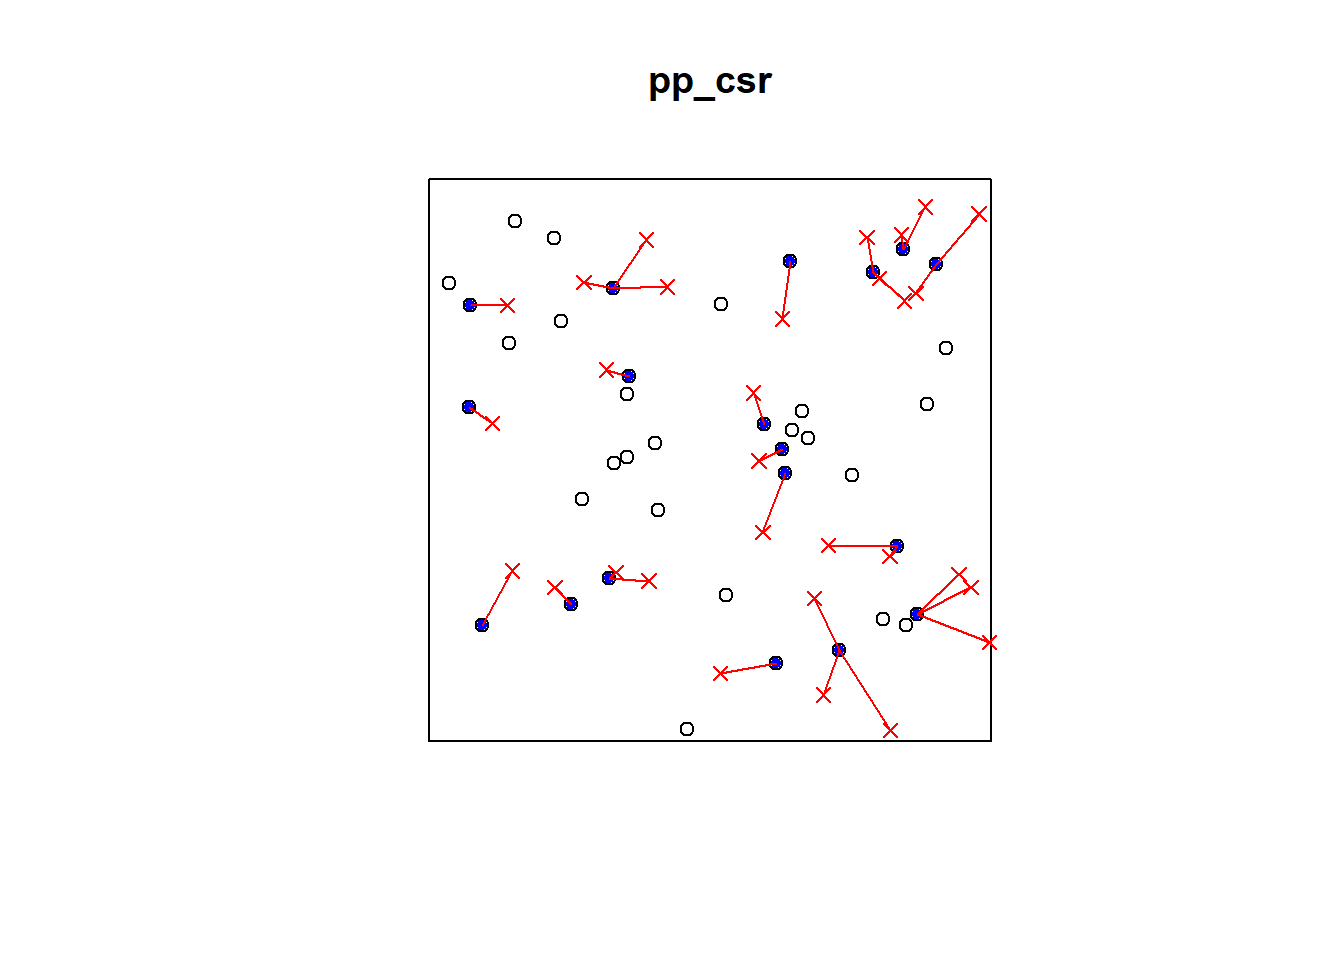
\includegraphics{Applied-Spatial-Data-Analysis_files/figure-latex/unnamed-chunk-45-1.pdf}

\hypertarget{cluster-pattern-1}{%
\subsubsection{Cluster Pattern}\label{cluster-pattern-1}}

\begin{Shaded}
\begin{Highlighting}[]
\KeywordTok{plot}\NormalTok{(pp_cluster)}
\KeywordTok{points}\NormalTok{(randompoints, }\DataTypeTok{col =} \StringTok{"blue"}\NormalTok{, }\DataTypeTok{pch=}\DecValTok{3}\NormalTok{)}
\end{Highlighting}
\end{Shaded}

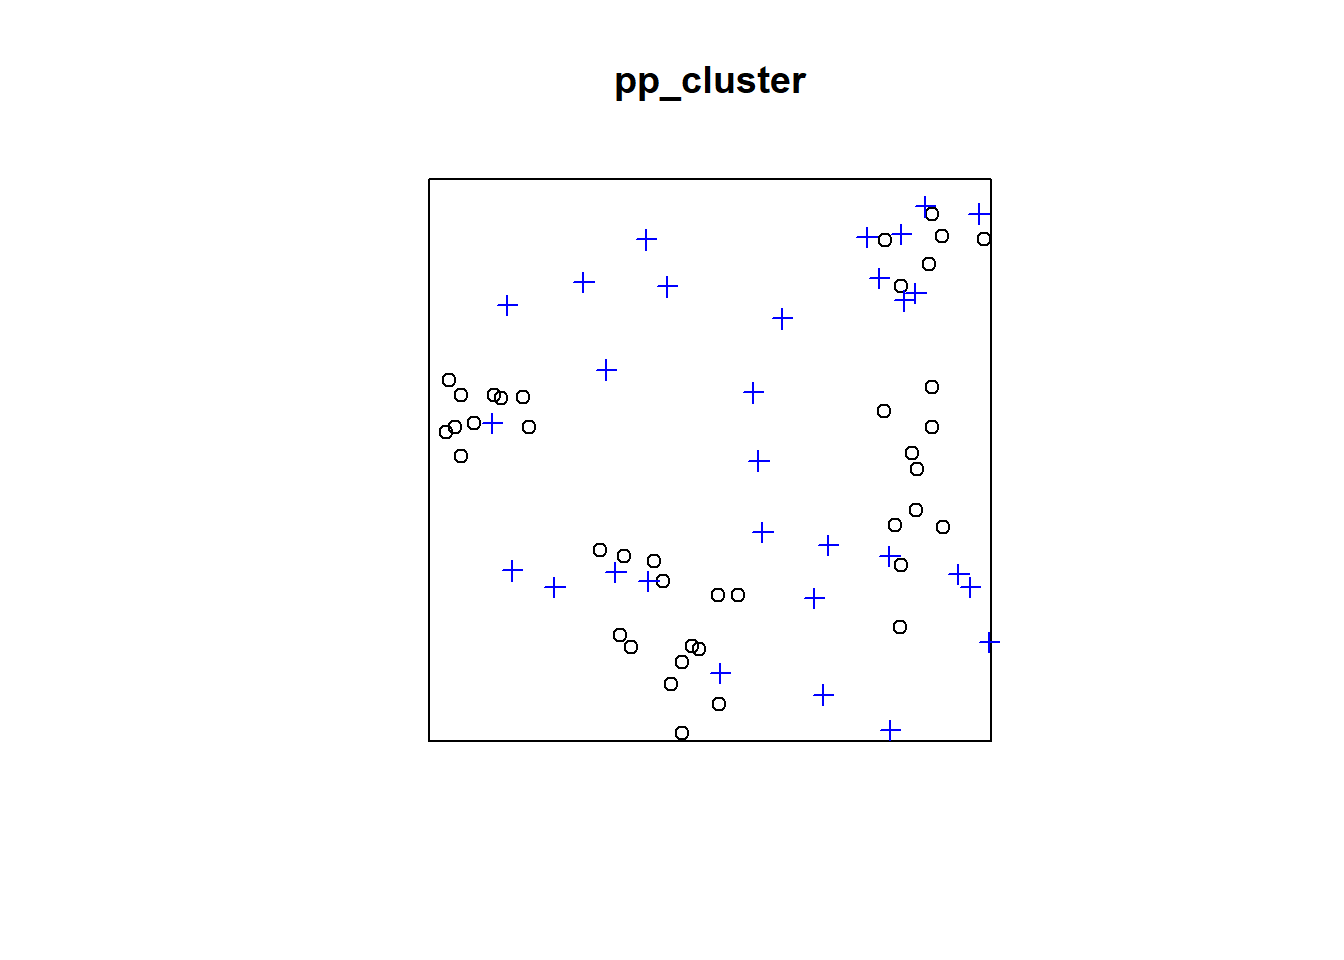
\includegraphics{Applied-Spatial-Data-Analysis_files/figure-latex/unnamed-chunk-46-1.pdf}

\begin{Shaded}
\begin{Highlighting}[]
\NormalTok{p2e_distances_cluster =}\StringTok{ }\OtherTok{NULL}
\NormalTok{mins_cluster =}\StringTok{ }\OtherTok{NULL}
\NormalTok{xy_cluster =}\StringTok{ }\KeywordTok{cbind}\NormalTok{(pp_cluster}\OperatorTok{$}\NormalTok{x, pp_cluster}\OperatorTok{$}\NormalTok{y)}

\ControlFlowTok{for}\NormalTok{(i }\ControlFlowTok{in} \DecValTok{1}\OperatorTok{:}\KeywordTok{dim}\NormalTok{(randompoints)[}\DecValTok{1}\NormalTok{])\{}
\NormalTok{dist1 =}\StringTok{ }\KeywordTok{matrix}\NormalTok{(}\KeywordTok{pairdist}\NormalTok{(}\KeywordTok{rbind}\NormalTok{(randompoints[i,],xy_cluster)),}\DecValTok{41}\NormalTok{)}

\NormalTok{p2e_distances_cluster =}\StringTok{ }\KeywordTok{c}\NormalTok{(p2e_distances_cluster,}\KeywordTok{min}\NormalTok{(dist1[}\DecValTok{2}\OperatorTok{:}\DecValTok{41}\NormalTok{,}\DecValTok{1}\NormalTok{]))}
\NormalTok{mins_cluster =}\StringTok{ }\KeywordTok{c}\NormalTok{(mins_cluster,}\KeywordTok{which.min}\NormalTok{(dist1[}\DecValTok{2}\OperatorTok{:}\DecValTok{41}\NormalTok{,}\DecValTok{1}\NormalTok{]))}
\NormalTok{\}}


\KeywordTok{plot}\NormalTok{(pp_cluster)}
\NormalTok{ord <-}\StringTok{ }\KeywordTok{rev}\NormalTok{(}\KeywordTok{order}\NormalTok{(p2e_distances_cluster))}
\NormalTok{far25 <-}\StringTok{ }\DecValTok{1}\OperatorTok{:}\KeywordTok{dim}\NormalTok{(randompoints)[}\DecValTok{1}\NormalTok{]}
\NormalTok{neighbors <-}\StringTok{ }\NormalTok{mins_cluster}
\KeywordTok{points}\NormalTok{(randompoints, }\DataTypeTok{col=}\StringTok{'red'}\NormalTok{, }\DataTypeTok{pch=}\DecValTok{4}\NormalTok{)}
\KeywordTok{points}\NormalTok{(xy_cluster[mins_cluster, ], }\DataTypeTok{col=}\StringTok{'blue'}\NormalTok{, }\DataTypeTok{pch=}\DecValTok{20}\NormalTok{)}
\CommentTok{# drawing the lines, easiest via a loop}
\ControlFlowTok{for}\NormalTok{ (i }\ControlFlowTok{in}\NormalTok{ far25) \{}
  \KeywordTok{lines}\NormalTok{(}\KeywordTok{rbind}\NormalTok{(xy_cluster[mins_cluster[i], ], randompoints[i, ]), }\DataTypeTok{col=}\StringTok{'red'}\NormalTok{)}
\NormalTok{\}}
\end{Highlighting}
\end{Shaded}

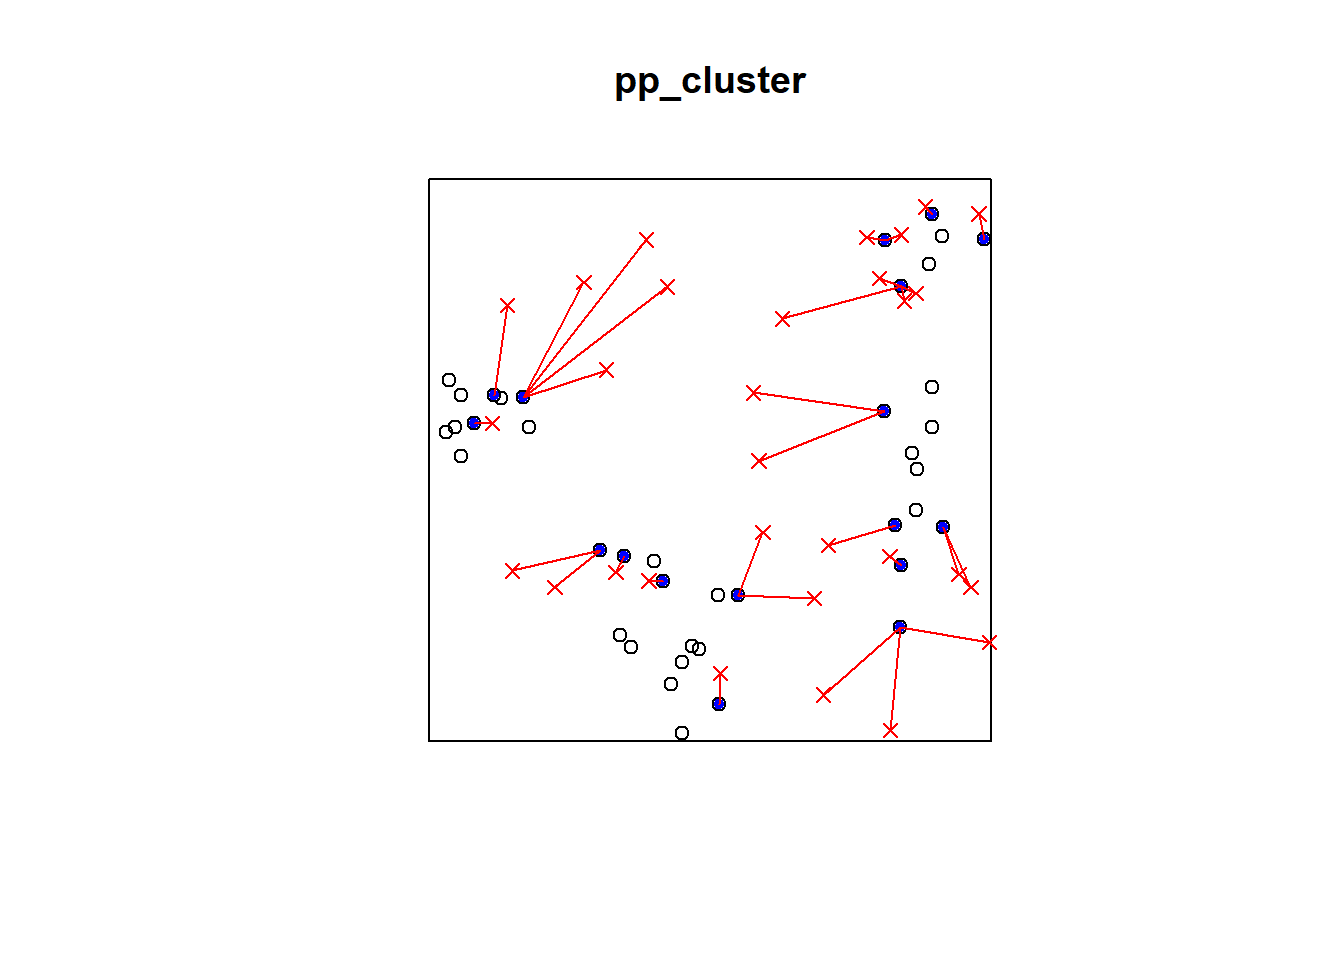
\includegraphics{Applied-Spatial-Data-Analysis_files/figure-latex/unnamed-chunk-47-1.pdf}

\hypertarget{regular-pattern-1}{%
\subsubsection{Regular Pattern}\label{regular-pattern-1}}

\begin{Shaded}
\begin{Highlighting}[]
\NormalTok{p2e_distances_regular =}\StringTok{ }\OtherTok{NULL}
\NormalTok{p2e_mins_regular =}\StringTok{ }\OtherTok{NULL}
\NormalTok{xy_regular =}\StringTok{ }\KeywordTok{cbind}\NormalTok{(pp_regular}\OperatorTok{$}\NormalTok{x, pp_regular}\OperatorTok{$}\NormalTok{y)}


\ControlFlowTok{for}\NormalTok{(i }\ControlFlowTok{in} \DecValTok{1}\OperatorTok{:}\KeywordTok{dim}\NormalTok{(randompoints)[}\DecValTok{1}\NormalTok{])\{}
\NormalTok{dist1 =}\StringTok{ }\KeywordTok{matrix}\NormalTok{(}\KeywordTok{pairdist}\NormalTok{(}\KeywordTok{rbind}\NormalTok{(randompoints[i,],xy_regular)),}\DecValTok{41}\NormalTok{)}

\NormalTok{p2e_distances_regular =}\StringTok{ }\KeywordTok{c}\NormalTok{(p2e_distances_regular,}\KeywordTok{min}\NormalTok{(dist1[}\DecValTok{2}\OperatorTok{:}\DecValTok{41}\NormalTok{,}\DecValTok{1}\NormalTok{]))}
\NormalTok{p2e_mins_regular =}\StringTok{ }\KeywordTok{c}\NormalTok{(p2e_mins_regular,}\KeywordTok{which.min}\NormalTok{(dist1[}\DecValTok{2}\OperatorTok{:}\DecValTok{41}\NormalTok{,}\DecValTok{1}\NormalTok{]))}
\NormalTok{\}}


\KeywordTok{plot}\NormalTok{(pp_regular)}
\NormalTok{ord <-}\StringTok{ }\KeywordTok{rev}\NormalTok{(}\KeywordTok{order}\NormalTok{(p2e_distances_regular))}
\NormalTok{far25 <-}\StringTok{ }\DecValTok{1}\OperatorTok{:}\KeywordTok{dim}\NormalTok{(randompoints)[}\DecValTok{1}\NormalTok{]}
\NormalTok{neighbors <-}\StringTok{ }\NormalTok{p2e_mins_regular}
\KeywordTok{points}\NormalTok{(randompoints, }\DataTypeTok{col=}\StringTok{'red'}\NormalTok{, }\DataTypeTok{pch=}\DecValTok{4}\NormalTok{)}
\KeywordTok{points}\NormalTok{(xy_regular[p2e_mins_regular, ], }\DataTypeTok{col=}\StringTok{'blue'}\NormalTok{, }\DataTypeTok{pch=}\DecValTok{20}\NormalTok{)}
\CommentTok{# drawing the lines, easiest via a loop}
\ControlFlowTok{for}\NormalTok{ (i }\ControlFlowTok{in}\NormalTok{ far25) \{}
  \KeywordTok{lines}\NormalTok{(}\KeywordTok{rbind}\NormalTok{(xy_regular[p2e_mins_regular[i], ], randompoints[i, ]), }\DataTypeTok{col=}\StringTok{'red'}\NormalTok{)}
\NormalTok{\}}
\end{Highlighting}
\end{Shaded}

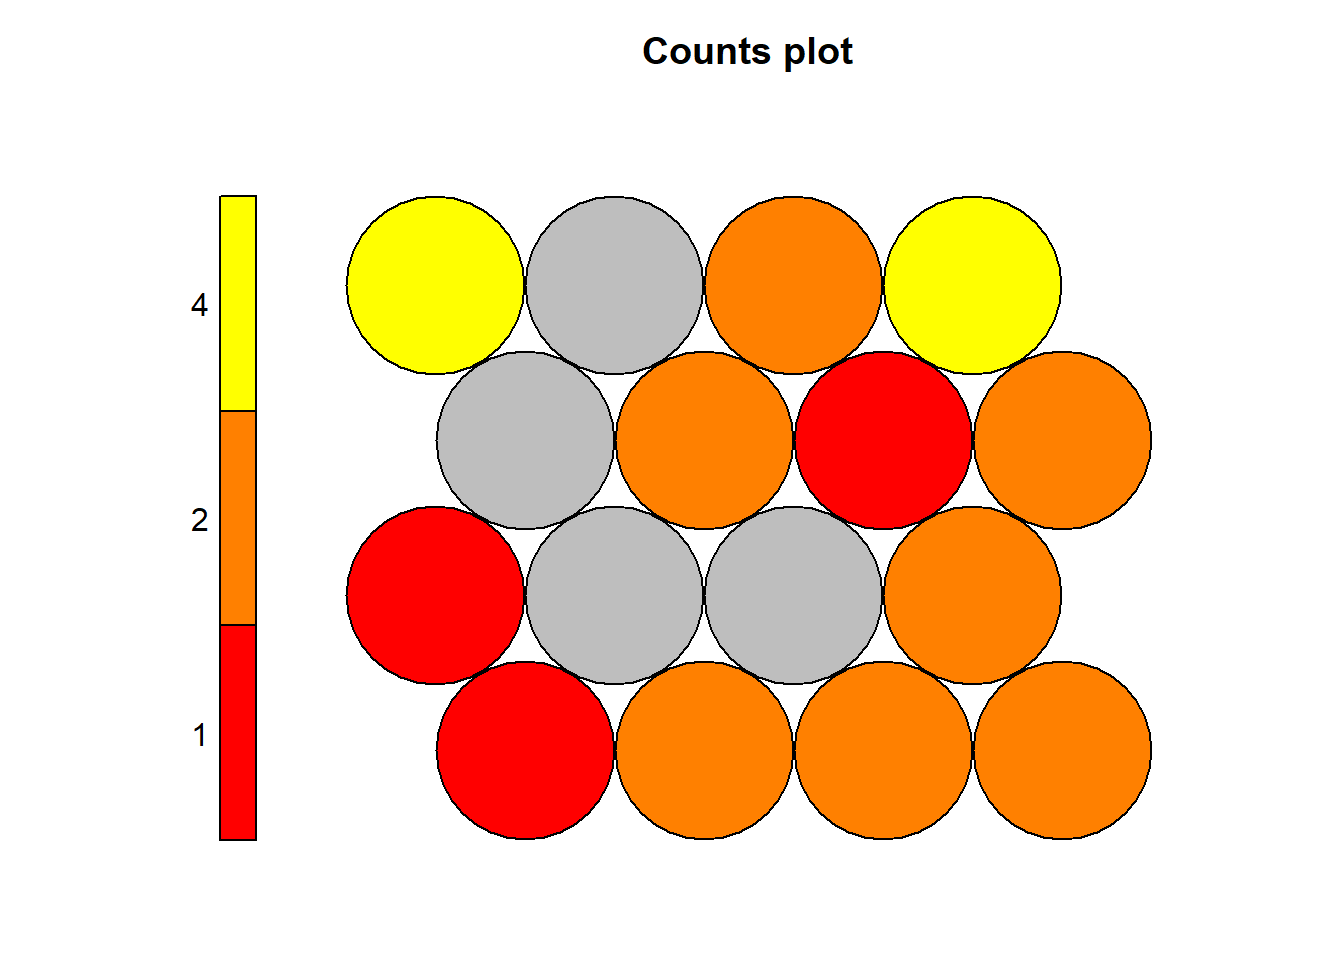
\includegraphics{Applied-Spatial-Data-Analysis_files/figure-latex/unnamed-chunk-48-1.pdf}

\hypertarget{clark-and-evans-index-and-test}{%
\subsection{Clark and Evans Index and Test}\label{clark-and-evans-index-and-test}}

\hypertarget{csr-pattern-2}{%
\subsubsection{CSR Pattern}\label{csr-pattern-2}}

\begin{Shaded}
\begin{Highlighting}[]
\KeywordTok{clarkevans}\NormalTok{(pp_csr)}
\end{Highlighting}
\end{Shaded}

\begin{verbatim}
##     naive  Donnelly       cdf 
## 1.0135515 0.9443703 0.9719128
\end{verbatim}

\begin{Shaded}
\begin{Highlighting}[]
\KeywordTok{clarkevans.test}\NormalTok{(pp_csr)}
\end{Highlighting}
\end{Shaded}

\begin{verbatim}
## 
## 	Clark-Evans test
## 	No edge correction
## 	Z-test
## 
## data:  pp_csr
## R = 1.0136, p-value = 0.8698
## alternative hypothesis: two-sided
\end{verbatim}

\hypertarget{cluster-pattern-2}{%
\subsubsection{Cluster Pattern}\label{cluster-pattern-2}}

\begin{Shaded}
\begin{Highlighting}[]
\KeywordTok{clarkevans}\NormalTok{(pp_cluster)}
\end{Highlighting}
\end{Shaded}

\begin{verbatim}
##     naive  Donnelly       cdf 
## 0.5852722 0.5453237 0.5621148
\end{verbatim}

\begin{Shaded}
\begin{Highlighting}[]
\KeywordTok{clarkevans.test}\NormalTok{(pp_cluster)}
\end{Highlighting}
\end{Shaded}

\begin{verbatim}
## 
## 	Clark-Evans test
## 	No edge correction
## 	Z-test
## 
## data:  pp_cluster
## R = 0.58527, p-value = 5.224e-07
## alternative hypothesis: two-sided
\end{verbatim}

\hypertarget{regular-pattern-2}{%
\subsubsection{Regular Pattern}\label{regular-pattern-2}}

\begin{Shaded}
\begin{Highlighting}[]
\KeywordTok{clarkevans}\NormalTok{(pp_regular)}
\end{Highlighting}
\end{Shaded}

\begin{verbatim}
##    naive Donnelly      cdf 
## 1.405457 1.309526 1.398362
\end{verbatim}

\begin{Shaded}
\begin{Highlighting}[]
\KeywordTok{clarkevans.test}\NormalTok{(pp_regular)}
\end{Highlighting}
\end{Shaded}

\begin{verbatim}
## 
## 	Clark-Evans test
## 	No edge correction
## 	Z-test
## 
## data:  pp_regular
## R = 1.4055, p-value = 9.309e-07
## alternative hypothesis: two-sided
\end{verbatim}

\hypertarget{g-function}{%
\section{G Function}\label{g-function}}

\hypertarget{simulated-csr-pattern-2}{%
\subsection{Simulated CSR Pattern}\label{simulated-csr-pattern-2}}

\begin{Shaded}
\begin{Highlighting}[]
\KeywordTok{plot}\NormalTok{(}\KeywordTok{Gest}\NormalTok{(pp_csr))}
\end{Highlighting}
\end{Shaded}

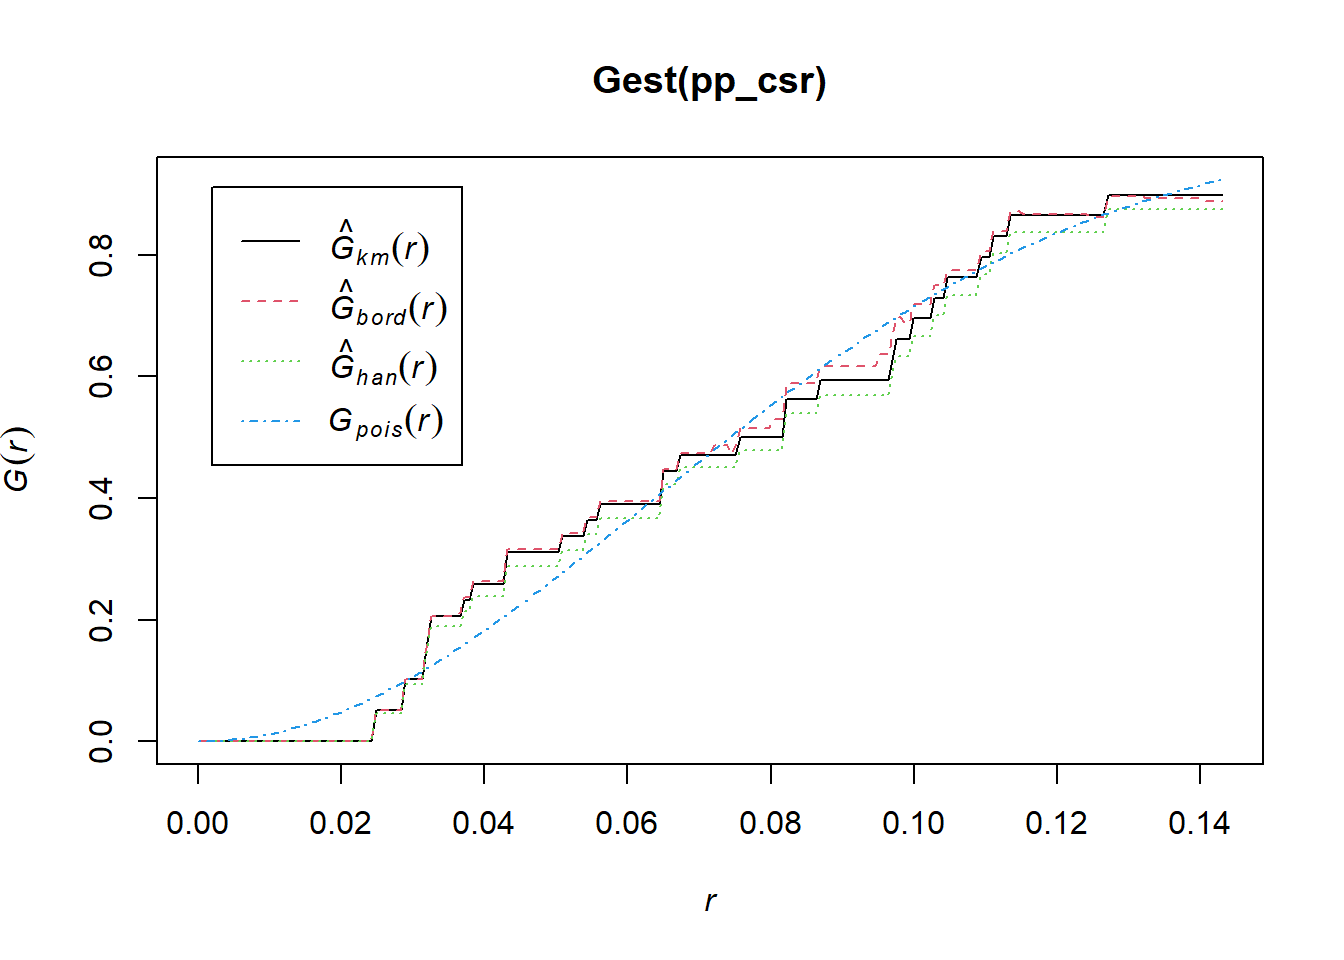
\includegraphics{Applied-Spatial-Data-Analysis_files/figure-latex/unnamed-chunk-52-1.pdf}

\hypertarget{simulated-regular-pattern-2}{%
\subsection{Simulated Regular Pattern}\label{simulated-regular-pattern-2}}

\begin{Shaded}
\begin{Highlighting}[]
\KeywordTok{plot}\NormalTok{(}\KeywordTok{Gest}\NormalTok{(pp_regular))}
\end{Highlighting}
\end{Shaded}

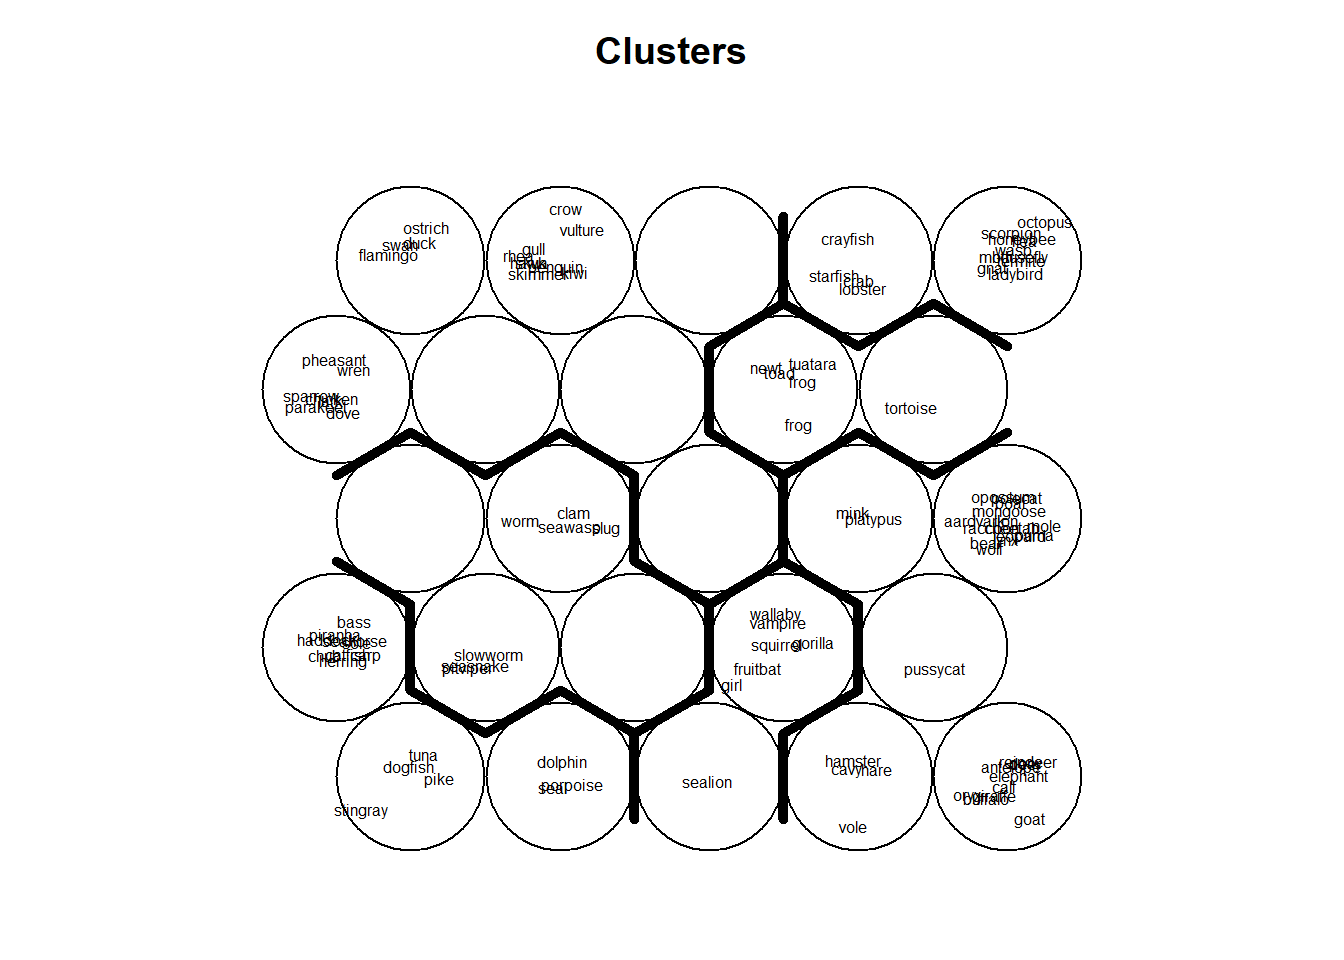
\includegraphics{Applied-Spatial-Data-Analysis_files/figure-latex/unnamed-chunk-53-1.pdf}

\hypertarget{simulated-cluster-pattern-2}{%
\subsection{Simulated Cluster Pattern}\label{simulated-cluster-pattern-2}}

\begin{Shaded}
\begin{Highlighting}[]
\KeywordTok{plot}\NormalTok{(}\KeywordTok{Gest}\NormalTok{(pp_cluster))}
\end{Highlighting}
\end{Shaded}

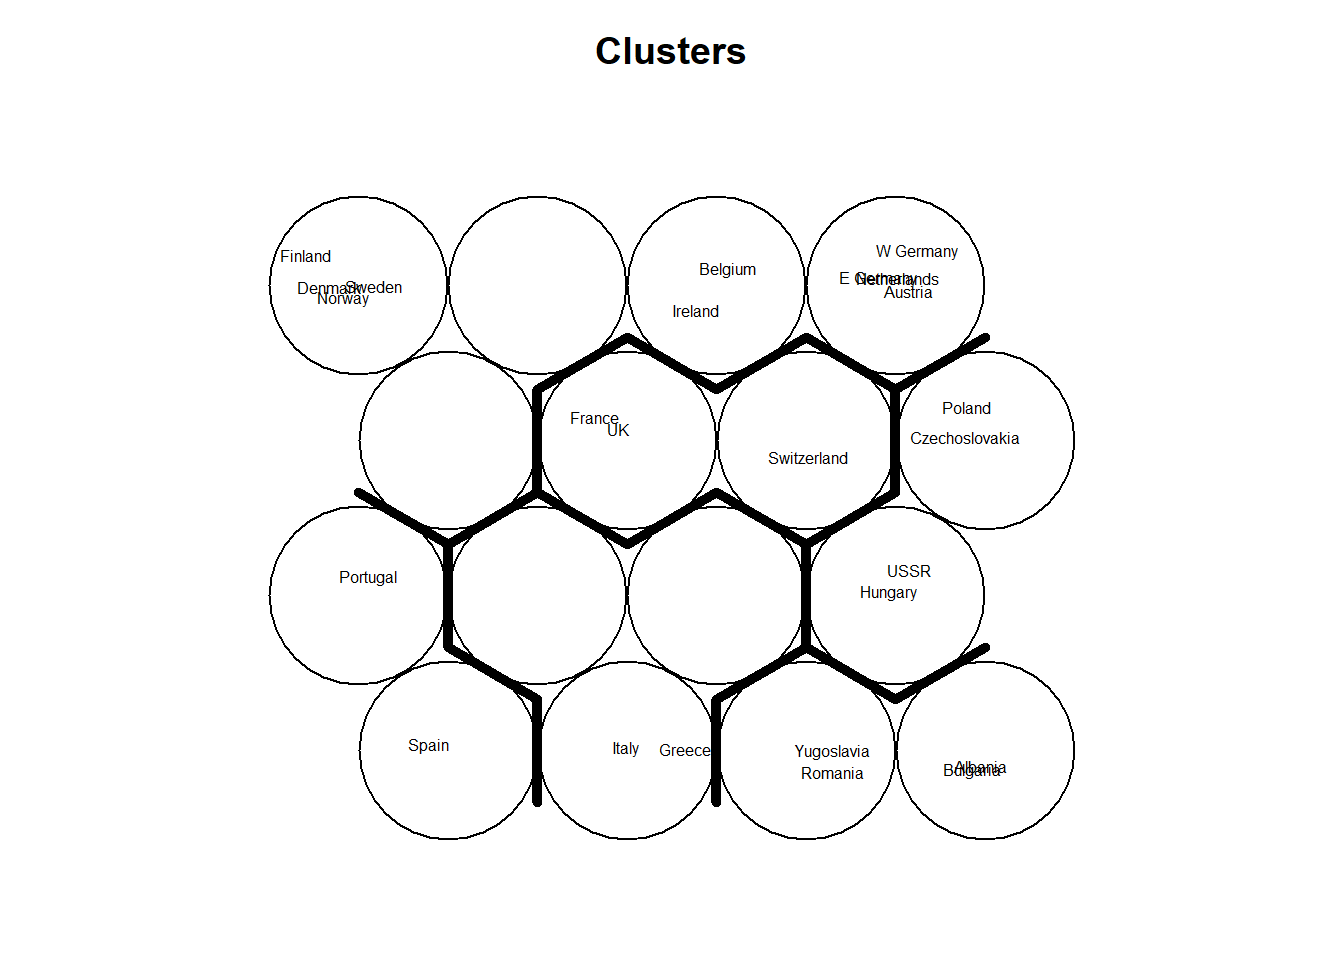
\includegraphics{Applied-Spatial-Data-Analysis_files/figure-latex/unnamed-chunk-54-1.pdf}

\hypertarget{f-function}{%
\section{F Function}\label{f-function}}

\hypertarget{simulated-csr-pattern-3}{%
\subsection{Simulated CSR Pattern}\label{simulated-csr-pattern-3}}

\begin{Shaded}
\begin{Highlighting}[]
\KeywordTok{plot}\NormalTok{(}\KeywordTok{Fest}\NormalTok{(pp_csr))}
\end{Highlighting}
\end{Shaded}

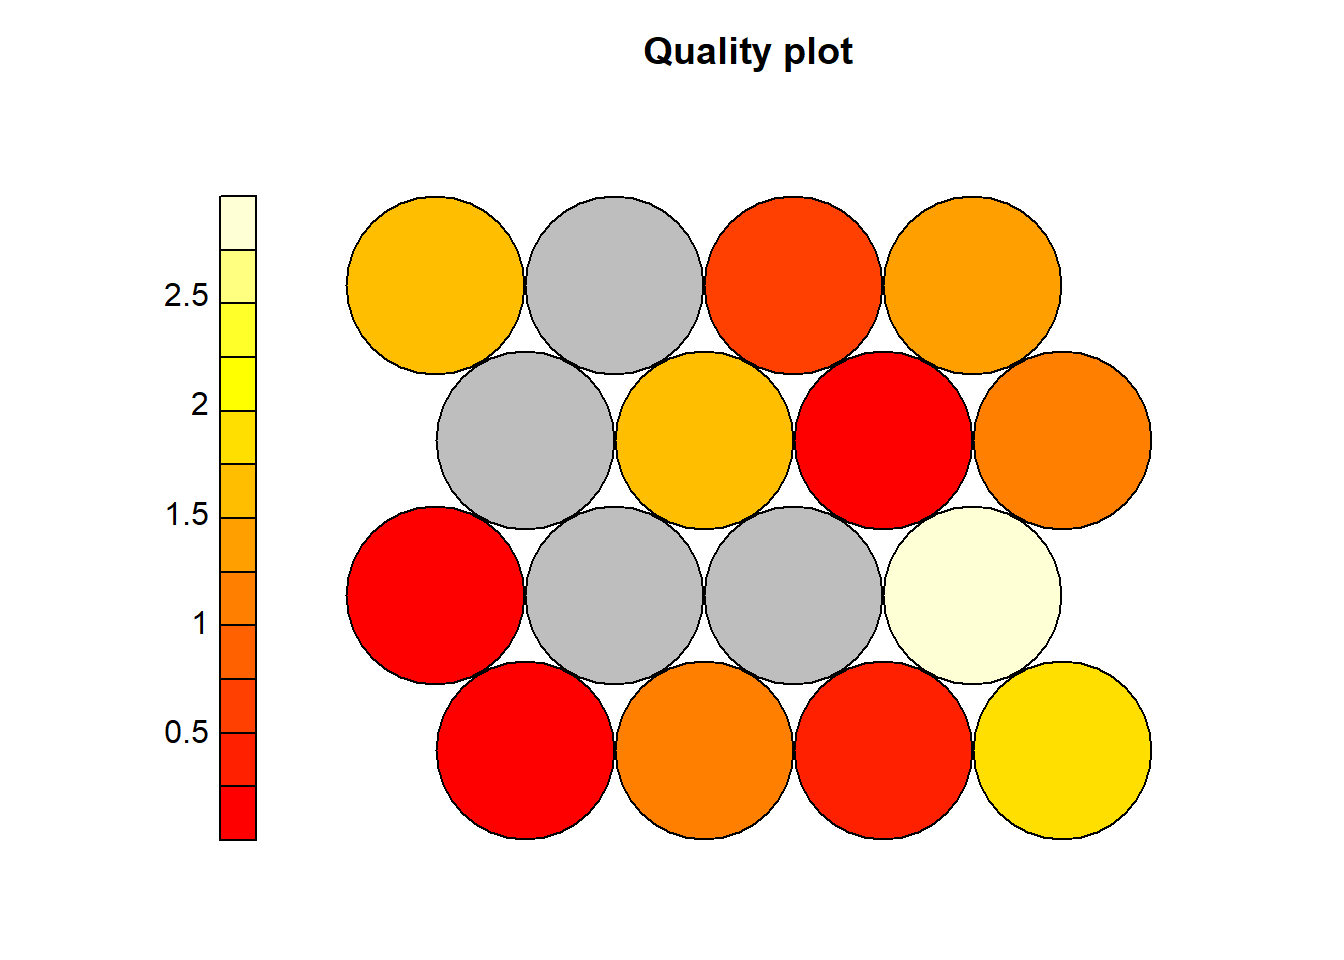
\includegraphics{Applied-Spatial-Data-Analysis_files/figure-latex/unnamed-chunk-55-1.pdf}

\hypertarget{simulated-regular-pattern-3}{%
\subsection{Simulated Regular Pattern}\label{simulated-regular-pattern-3}}

\begin{Shaded}
\begin{Highlighting}[]
\KeywordTok{plot}\NormalTok{(}\KeywordTok{Fest}\NormalTok{(pp_regular))}
\end{Highlighting}
\end{Shaded}

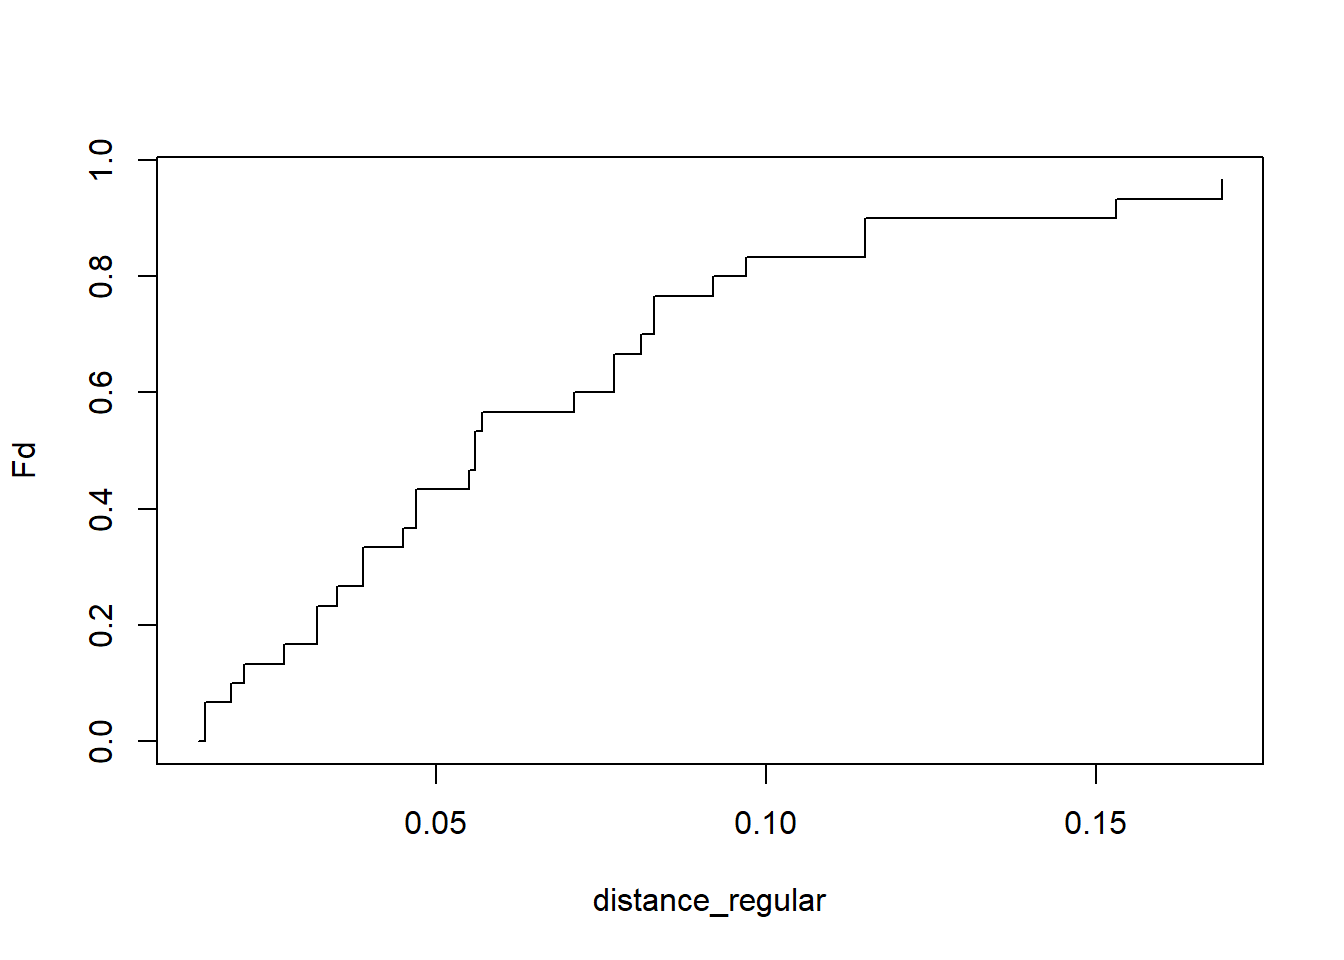
\includegraphics{Applied-Spatial-Data-Analysis_files/figure-latex/unnamed-chunk-56-1.pdf}

\hypertarget{simulated-cluster-pattern-3}{%
\subsection{Simulated Cluster Pattern}\label{simulated-cluster-pattern-3}}

\begin{Shaded}
\begin{Highlighting}[]
\KeywordTok{plot}\NormalTok{(}\KeywordTok{Fest}\NormalTok{(pp_cluster))}
\end{Highlighting}
\end{Shaded}

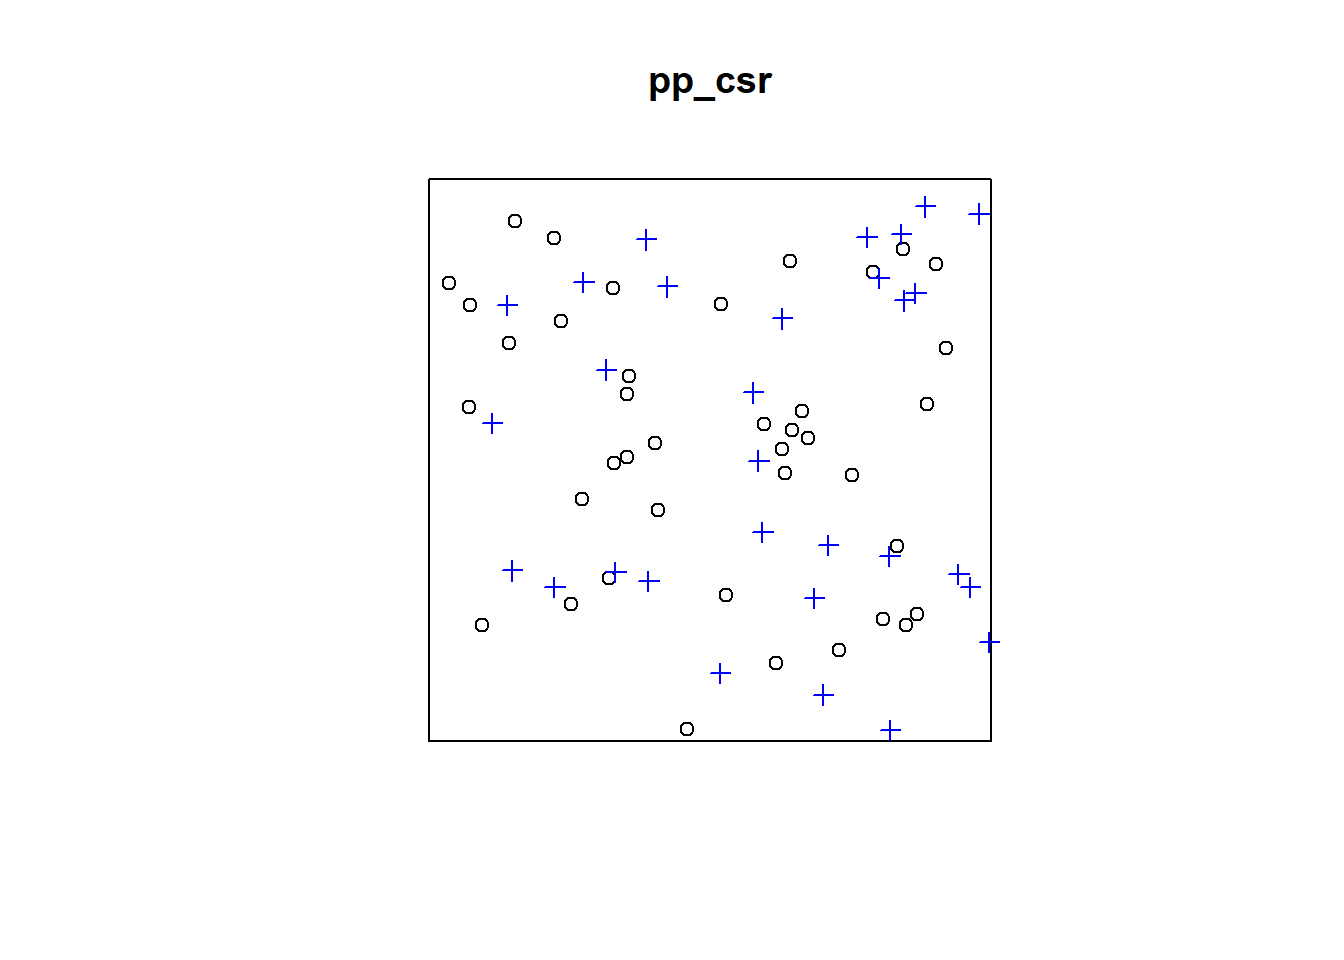
\includegraphics{Applied-Spatial-Data-Analysis_files/figure-latex/unnamed-chunk-57-1.pdf}

\hypertarget{ripleys-k-function}{%
\section{Ripley's K Function}\label{ripleys-k-function}}

\hypertarget{simulated-csr-pattern-4}{%
\subsection{Simulated CSR Pattern}\label{simulated-csr-pattern-4}}

\begin{Shaded}
\begin{Highlighting}[]
\NormalTok{K <-}\StringTok{ }\KeywordTok{Kest}\NormalTok{(pp_csr)}
\KeywordTok{plot}\NormalTok{(K, }\DataTypeTok{main=}\OtherTok{NULL}\NormalTok{, }\DataTypeTok{las=}\DecValTok{1}\NormalTok{, }\DataTypeTok{legendargs=}\KeywordTok{list}\NormalTok{(}\DataTypeTok{cex=}\FloatTok{0.8}\NormalTok{, }\DataTypeTok{xpd=}\OtherTok{TRUE}\NormalTok{, }\DataTypeTok{inset=}\KeywordTok{c}\NormalTok{(}\FloatTok{1.01}\NormalTok{, }\DecValTok{0}\NormalTok{) ))}
\end{Highlighting}
\end{Shaded}

\begin{verbatim}
## Warning in min(D[scaledlegbox]): no non-missing arguments to min; returning Inf
\end{verbatim}

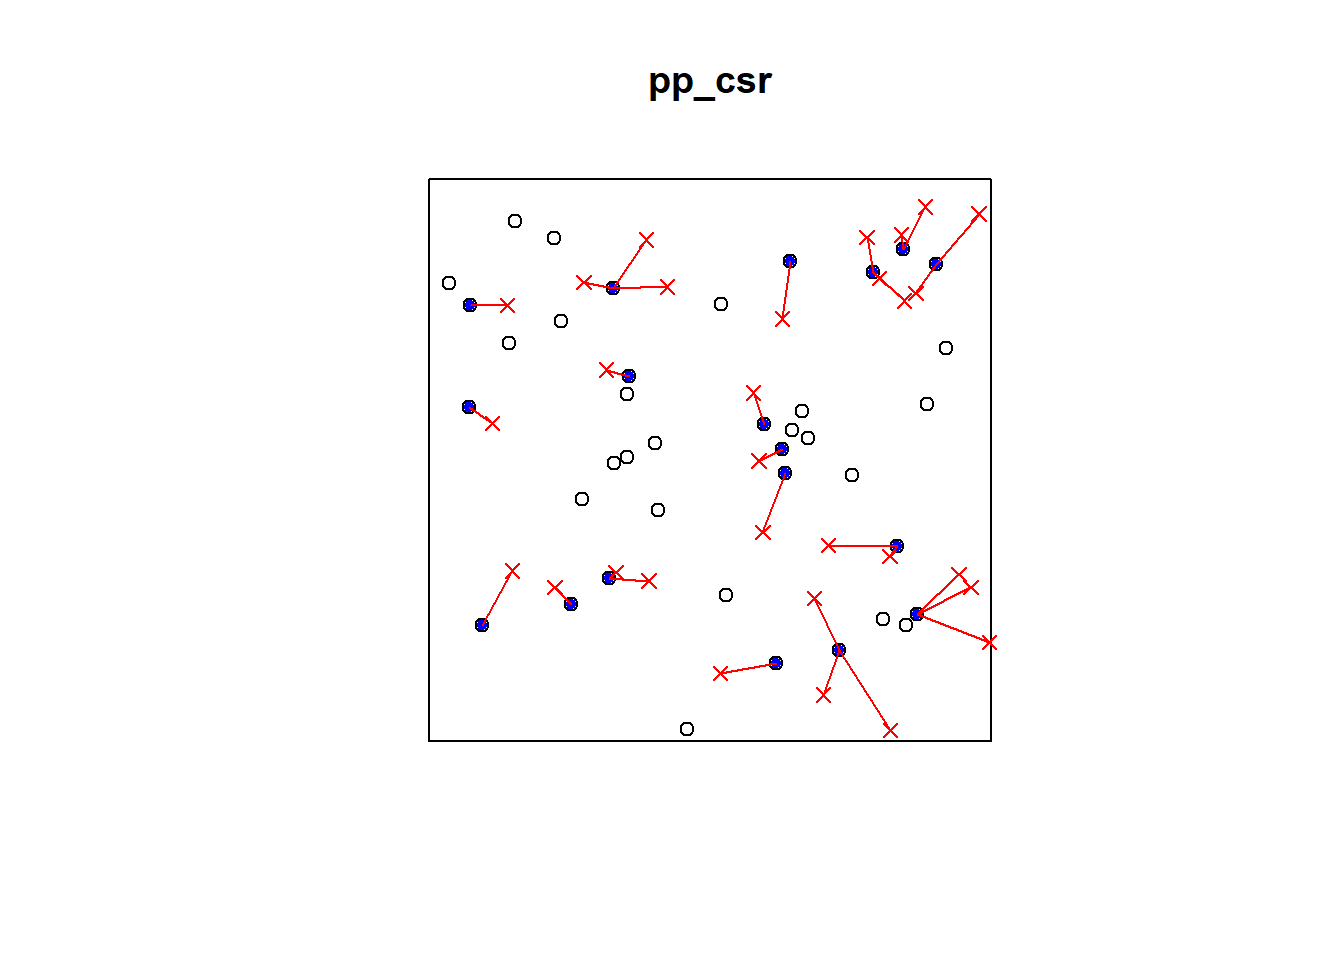
\includegraphics{Applied-Spatial-Data-Analysis_files/figure-latex/unnamed-chunk-58-1.pdf}

\hypertarget{simulated-regular-pattern-4}{%
\subsection{Simulated Regular Pattern}\label{simulated-regular-pattern-4}}

\begin{Shaded}
\begin{Highlighting}[]
\NormalTok{K <-}\StringTok{ }\KeywordTok{Kest}\NormalTok{(pp_regular)}
\KeywordTok{plot}\NormalTok{(K, }\DataTypeTok{main=}\OtherTok{NULL}\NormalTok{, }\DataTypeTok{las=}\DecValTok{1}\NormalTok{, }\DataTypeTok{legendargs=}\KeywordTok{list}\NormalTok{(}\DataTypeTok{cex=}\FloatTok{0.8}\NormalTok{, }\DataTypeTok{xpd=}\OtherTok{TRUE}\NormalTok{, }\DataTypeTok{inset=}\KeywordTok{c}\NormalTok{(}\FloatTok{1.01}\NormalTok{, }\DecValTok{0}\NormalTok{) ))}
\end{Highlighting}
\end{Shaded}

\begin{verbatim}
## Warning in min(D[scaledlegbox]): no non-missing arguments to min; returning Inf
\end{verbatim}

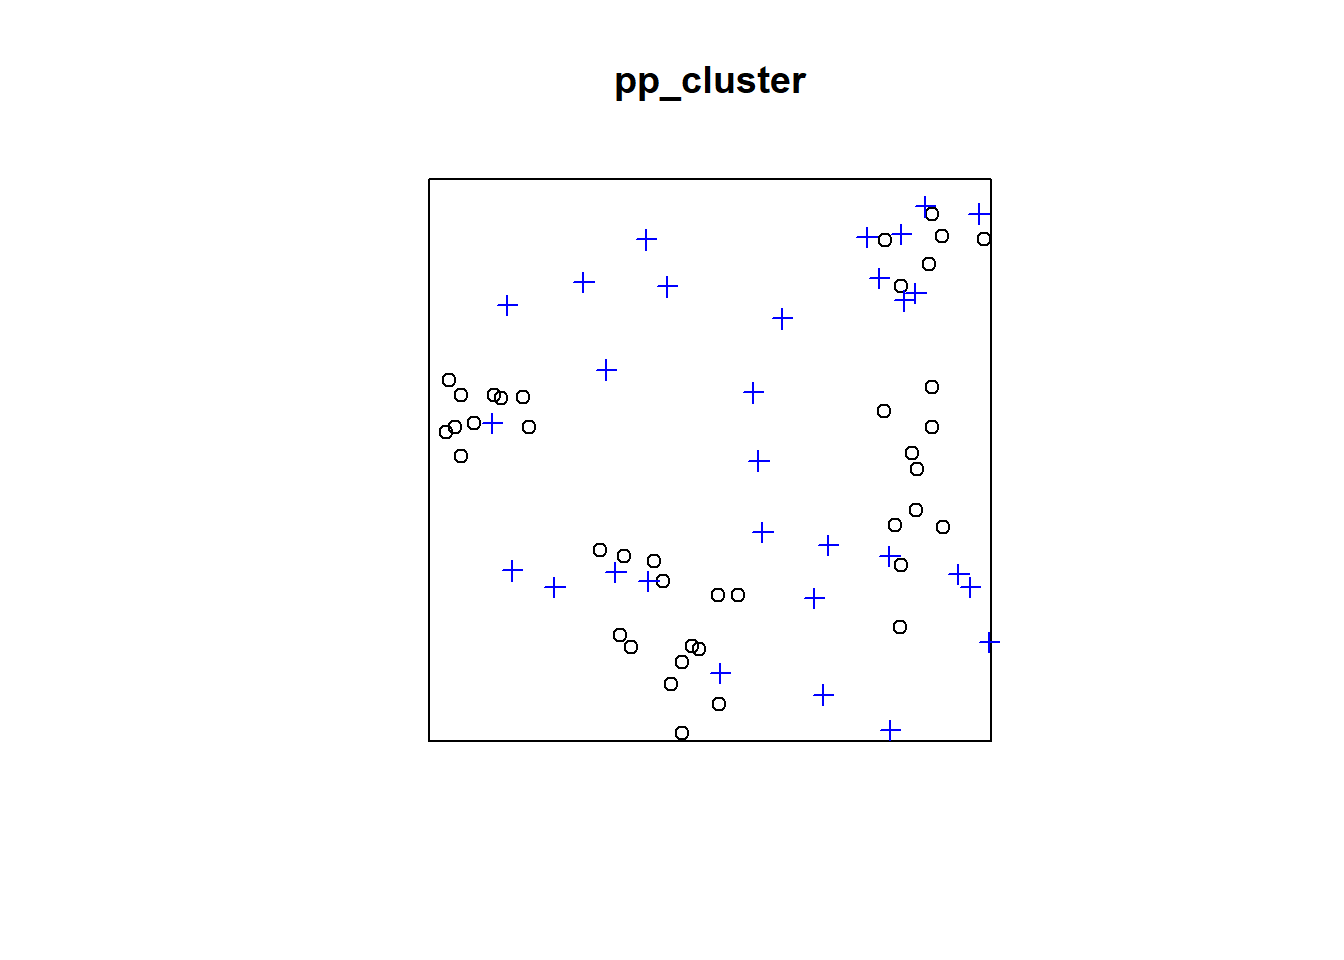
\includegraphics{Applied-Spatial-Data-Analysis_files/figure-latex/unnamed-chunk-59-1.pdf}

\hypertarget{simulated-cluster-pattern-4}{%
\subsection{Simulated Cluster Pattern}\label{simulated-cluster-pattern-4}}

\begin{Shaded}
\begin{Highlighting}[]
\NormalTok{K <-}\StringTok{ }\KeywordTok{Kest}\NormalTok{(pp_cluster)}
\KeywordTok{plot}\NormalTok{(K, }\DataTypeTok{main=}\OtherTok{NULL}\NormalTok{, }\DataTypeTok{las=}\DecValTok{1}\NormalTok{, }\DataTypeTok{legendargs=}\KeywordTok{list}\NormalTok{(}\DataTypeTok{cex=}\FloatTok{0.8}\NormalTok{, }\DataTypeTok{xpd=}\OtherTok{TRUE}\NormalTok{, }\DataTypeTok{inset=}\KeywordTok{c}\NormalTok{(}\FloatTok{1.01}\NormalTok{, }\DecValTok{0}\NormalTok{) ))}
\end{Highlighting}
\end{Shaded}

\begin{verbatim}
## Warning in min(D[scaledlegbox]): no non-missing arguments to min; returning Inf
\end{verbatim}

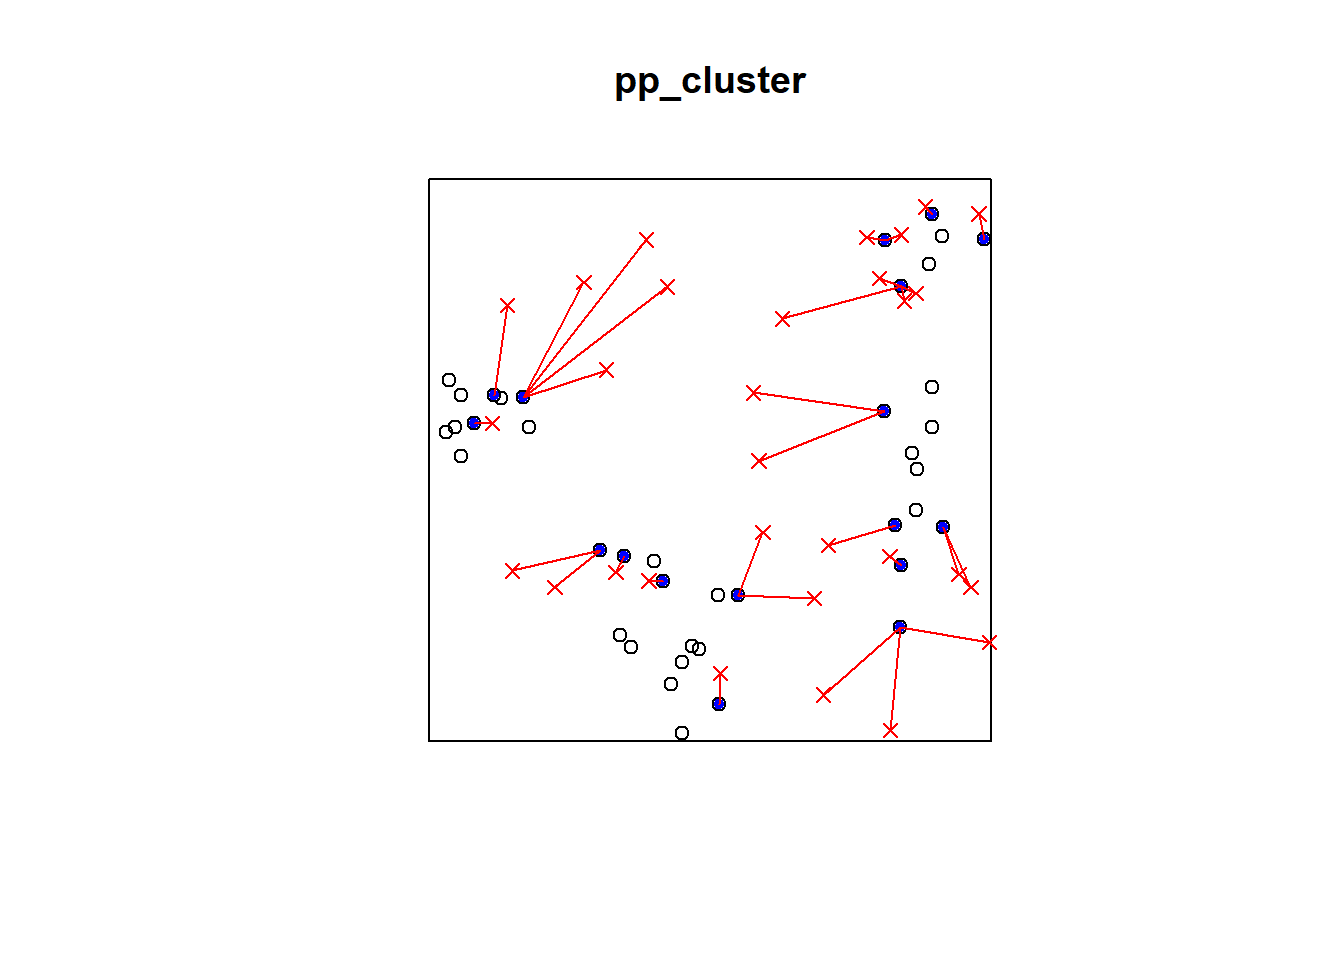
\includegraphics{Applied-Spatial-Data-Analysis_files/figure-latex/unnamed-chunk-60-1.pdf}

\hypertarget{references}{%
\section{References:}\label{references}}

\begin{itemize}
\item
  \href{https://rpubs.com/spring19cp6521/Week11_Wednesday1}{Point Pattern Analysis by Yongsung Lee}
\item
  \href{https://bookdown.org/lexcomber/brunsdoncomber2e/Ch6.html}{An Introduction to Spatial Analysis and Mapping in R 2nd edition by Chris Brunsdon and Lex Comber}
\item
  \href{https://mgimond.github.io/Spatial/point-pattern-analysis-in-r.html}{SPP in R by Manuel Gimond}
\end{itemize}

\hypertarget{spatial-lattice-data-analysis}{%
\chapter{Spatial Lattice Data Analysis}\label{spatial-lattice-data-analysis}}

For this section, please update your browser on the 20th of October Tuesday.

  \bibliography{book.bib,packages.bib}

\end{document}
